
\documentclass[a4paper,12pt,twoside]{report}
\usepackage[left=3cm,right=2cm,top=4cm,bottom=3cm]{geometry}
\usepackage[utf8]{inputenc}
\usepackage[spanish]{babel}
\usepackage{amsthm}
\usepackage{amsmath}
\usepackage{amsfonts}
\usepackage{pgf,tikz}
\usepackage{graphicx}
\usepackage{float}
\usepackage{cite}
\usepackage{enumerate}
\usepackage{courier}
\usepackage{listings}
\usepackage{color}

\definecolor{codegreen}{rgb}{0,0.6,0}
\definecolor{codegray}{rgb}{0.5,0.5,0.5}
\definecolor{codepurple}{rgb}{0.58,0,0.82}
\definecolor{backcolour}{rgb}{0.95,0.95,0.92}

\lstdefinestyle{mystyle}{
	backgroundcolor=\color{backcolour},   
	commentstyle=\color{codegreen},
	keywordstyle=\color{magenta},
	numberstyle=\tiny\color{codegray},
	stringstyle=\color{codepurple},
	basicstyle=\footnotesize\ttfamily,
	breakatwhitespace=false,         
	breaklines=true,                 
	captionpos=b,                    
	keepspaces=true,                 
	numbers=left,                    
	numbersep=5pt,                  
	showspaces=false,                
	showstringspaces=false,
	showtabs=false,                  
	tabsize=2
}

\lstset{style=mystyle}
\usepackage{hyperref}
\graphicspath{ {/home/booort/Escritorio/tfg/images/} }
\usepackage[toc,page]{appendix}


\usepackage{graphicx}
\usepackage{verbatim}
\usepackage{latexsym}
\usepackage{mathchars}
\usepackage{setspace}


\setlength{\parskip}{\medskipamount}  % a little space before a \par
\setlength{\parindent}{0pt}	      % don't indent first lines of paragraphs

%UHEAD.STY  If this is included after \documentstyle{report}, it adds
% an underlined heading style to the LaTeX report style.
% \pagestyle{uheadings} will put underlined headings at the top
% of each page. The right page headings are the Chapter titles and
% the left page titles are supplied by \def\lefthead{text}.

% Ted Shapin, Dec. 17, 1986

\makeatletter
\def\chapapp2{Capítulo}

\def\appendix{\par
 \setcounter{chapter}{0}
 \setcounter{section}{0}
 \def\chapapp2{Anexo}
 \def\@chapapp{Anexo}
 \def\thechapter{\Alph{chapter}}}

\def\ps@uheadings{\let\@mkboth\markboth
% modifications
\def\@oddhead{\protect\underline{\protect\makebox[\textwidth][l]
		{\sl\rightmark\hfill\rm\thepage}}}
\def\@oddfoot{}
\def\@evenfoot{}
\def\@evenhead{\protect\underline{\protect\makebox[\textwidth][l]
		{\rm\thepage\hfill\sl\leftmark}}}
% end of modifications
\def\chaptermark##1{\markboth {\ifnum \c@secnumdepth >\m@ne
 \chapapp2\ \thechapter. \ \fi ##1}{}}%
\def\sectionmark##1{\markright {\ifnum \c@secnumdepth >\z@
   \thesection. \ \fi ##1}}}
\makeatother



%%From: marcel@cs.caltech.edu (Marcel van der Goot)
%%Newsgroups: comp.text.tex
%%Subject: illegal modification of boxit.sty
%%Date: 28 Feb 92 01:10:02 GMT
%%Organization: California Institute of Technology (CS dept)
%%Nntp-Posting-Host: andromeda.cs.caltech.edu
%%
%%
%%Quite some time ago I posted a file boxit.sty; maybe it made it
%%to some archives, although I don't recall submitting it. It defines
%%	\begin{boxit}
%%	...
%%	\end{boxit}
%%to draw a box around `...', where the `...' can contain other
%%environments (e.g., a verbatim environment). Unfortunately, it had
%%a problem: it did not work if you used it in paragraph mode, i.e., it
%%only worked if there was an empty line in front of \begin{boxit}.
%%Luckily, that is easily corrected.
%%
%%HOWEVER, apparently someone noticed the problem, tried to correct it,
%%and then distributed this modified version. That would be fine with me,
%%except that:
%%1. There was no note in the file about this modification, it only has my
%%   name in it.
%%2. The modification is wrong: now it only works if there is *no* empty
%%   line in front of \begin{boxit}. In my opinion this bug is worse than
%%   the original one.
%%
%%In particular, the author of this modification tried to force an empty
%%line by inserting a `\\' in the definition of \Beginboxit. If you have
%%a version of boxit.sty with a `\\', please delete it. If you have my
%%old version of boxit.sty, please also delete it. Below is an improved
%%version.
%%
%%Thanks to Joe Armstrong for drawing my attention to the bug and to the
%%illegal version.
%%
%%                                          Marcel van der Goot
%% .---------------------------------------------------------------
%% | Blauw de viooltjes,                    marcel@cs.caltech.edu
%% |    Rood zijn de rozen;
%% | Een rijm kan gezet
%% |    Met plaksel en dozen.
%% |


% boxit.sty
% version: 27 Feb 1992
%
% Defines a boxit environment, which draws lines around its contents.
% Usage:
%   \begin{boxit}
%	... (text you want to be boxed, can contain other environments)
%   \end{boxit}
%
% The width of the box is the width of the contents.
% The boxit* environment behaves the same, except that the box will be
% at least as wide as a normal paragraph.
%
% The reason for writing it this way (rather than with the \boxit#1 macro
% from the TeXbook), is that now you can box verbatim text, as in
%   \begin{boxit}
%   \begin{verbatim}
%   this better come out in boxed verbatim mode ...
%   \end{verbatim}
%   \end{boxit}
%
%						Marcel van der Goot
%						marcel@cs.caltech.edu
%

\def\Beginboxit
   {\par
    \vbox\bgroup
	   \hrule
	   \hbox\bgroup
		  \vrule \kern1.2pt %
		  \vbox\bgroup\kern1.2pt
   }

\def\Endboxit{%
			      \kern1.2pt
		       \egroup
		  \kern1.2pt\vrule
		\egroup
	   \hrule
	 \egroup
   }	

\newenvironment{boxit}{\Beginboxit}{\Endboxit}
\newenvironment{boxit*}{\Beginboxit\hbox to\hsize{}}{\Endboxit}

\pagestyle{empty}

\setlength{\parskip}{2ex plus 0.5ex minus 0.2ex}
\setlength{\parindent}{0pt}

\makeatletter  %to avoid error messages generated by "\@". Makes Latex treat "@" like a letter

\linespread{1.2}
\def\submitdate#1{\gdef\@submitdate{#1}}

\def\maketitle{
  \begin{titlepage}{
    %\linespread{1.5}
    
\includegraphics[scale=0.2]{../../Escritorio/tfg/images/ugr}
    
    \Large Universidad de Granada \\
    %\linebreak
    Grado en Matemáticas \\
    %\linebreak
    Departamento de Matemática Aplicada
    \rm
    \vskip 1in
    \Large \bf \@title \par
    
  }
  \vskip 0.2in
  \par
  {\Large \@author}
  \vskip 0.1in
  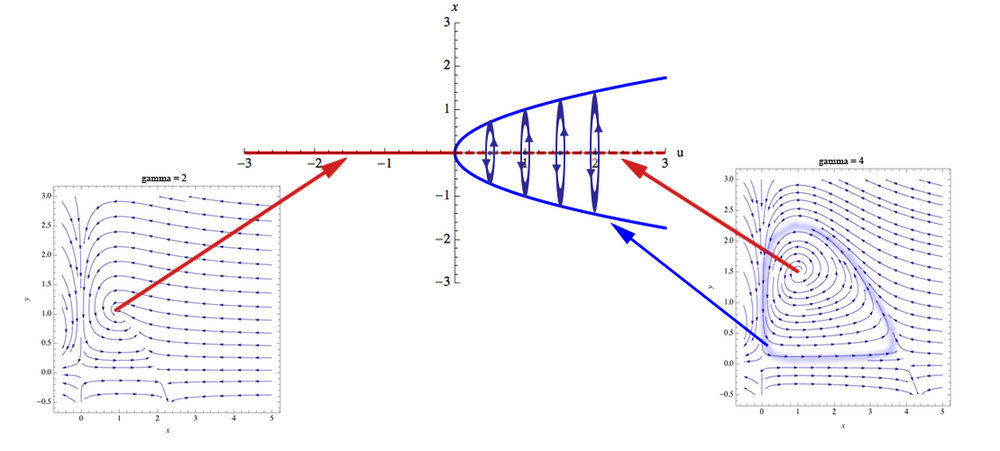
\includegraphics[scale=0.6]{../../Escritorio/tfg/images/portada}
  \vskip 1in
  \par
 
   \@submitdate
  \vfil
  \end{titlepage}
}

\def\titlepage{
  \newpage
  \centering
  \linespread{1}
  \normalsize
  \vbox to \vsize\bgroup\vbox to 9in\bgroup
}
\def\endtitlepage{
  \par
  \kern 0pt
  \egroup
  \vss
  \egroup
  \cleardoublepage
}

\def\abstract{
  \begin{center}{
    \large\bf Abstract}
  \end{center}
  \small
  %\def\baselinestretch{1.5}
  \linespread{1.5}
  \normalsize
}
\def\endabstract{
  \par
}

\newenvironment{acknowledgements}{
  \cleardoublepage
  \begin{center}{
    \large \bf Agradecimientos}
  \end{center}
  \small
  \linespread{1.5}
  \normalsize
}{\cleardoublepage}
\def\endacknowledgements{
  \par
}

\newenvironment{dedication}{
  \cleardoublepage
  \begin{center}{
    \large \bf Dedication}
  \end{center}
  \small
  \linespread{1.5}
  \normalsize
}{\cleardoublepage}
\def\enddedication{
  \par
}

\def\preface{
    \pagenumbering{roman}
    \pagestyle{plain}
    \doublespacing
}

\def\body{
    \cleardoublepage    
    \pagestyle{uheadings}
    \tableofcontents
    \pagestyle{plain}
    \cleardoublepage
    \pagestyle{uheadings}
    \listoftables
    \pagestyle{plain}
    \cleardoublepage
    \pagestyle{uheadings}
    \listoffigures
    \pagestyle{plain}
    \cleardoublepage
    \pagestyle{uheadings}
    \pagenumbering{arabic}
    \linespread{1.4}
}

\makeatother  %to avoid error messages generated by "\@". Makes Latex treat "@" like a letter


\newcommand{\ipc}{{\sf ipc}}

\newcommand{\Prob}{\bbbp}
\newcommand{\Real}{\bbbr}
\newcommand{\real}{\Real}
\newcommand{\Int}{\bbbz}
\newcommand{\Nat}{\bbbn}

\newcommand{\NN}{{\sf I\kern-0.14emN}}   % Natural numbers
\newcommand{\ZZ}{{\sf Z\kern-0.45emZ}}   % Integers
\newcommand{\QQQ}{{\sf C\kern-0.48emQ}}   % Rational numbers
\newcommand{\RR}{{\sf I\kern-0.14emR}}   % Real numbers
\newcommand{\KK}{{\cal K}}
\newcommand{\OO}{{\cal O}}
\newcommand{\AAA}{{\bf A}}
\newcommand{\HH}{{\bf H}}
\newcommand{\II}{{\bf I}}
\newcommand{\LL}{{\bf L}}
\newcommand{\PP}{{\bf P}}
\newcommand{\PPprime}{{\bf P'}}
\newcommand{\QQ}{{\bf Q}}
\newcommand{\UU}{{\bf U}}
\newcommand{\UUprime}{{\bf U'}}
\newcommand{\zzero}{{\bf 0}}
\newcommand{\ppi}{\mbox{\boldmath $\pi$}}
\newcommand{\aalph}{\mbox{\boldmath $\alpha$}}
\newcommand{\bb}{{\bf b}}
\newcommand{\ee}{{\bf e}}
\newcommand{\mmu}{\mbox{\boldmath $\mu$}}
\newcommand{\vv}{{\bf v}}
\newcommand{\xx}{{\bf x}}
\newcommand{\yy}{{\bf y}}
\newcommand{\zz}{{\bf z}}
\newcommand{\oomeg}{\mbox{\boldmath $\omega$}}
\newcommand{\res}{{\bf res}}
\newcommand{\cchi}{{\mbox{\raisebox{.4ex}{$\chi$}}}}
%\newcommand{\cchi}{{\cal X}}
%\newcommand{\cchi}{\mbox{\Large $\chi$}}

% Logical operators and symbols
\newcommand{\imply}{\Rightarrow}
\newcommand{\bimply}{\Leftrightarrow}
\newcommand{\union}{\cup}
\newcommand{\intersect}{\cap}
\newcommand{\boolor}{\vee}
\newcommand{\booland}{\wedge}
\newcommand{\boolimply}{\imply}
\newcommand{\boolbimply}{\bimply}
\newcommand{\boolnot}{\neg}
\newcommand{\boolsat}{\!\models}
\newcommand{\boolnsat}{\!\not\models}


\newcommand{\op}[1]{\mathrm{#1}}
\newcommand{\s}[1]{\ensuremath{\mathcal #1}}

% Properly styled differentiation and integration operators
\newcommand{\diff}[1]{\mathrm{\frac{d}{d\mathit{#1}}}}
\newcommand{\diffII}[1]{\mathrm{\frac{d^2}{d\mathit{#1}^2}}}
\newcommand{\intg}[4]{\int_{#3}^{#4} #1 \, \mathrm{d}#2}
\newcommand{\intgd}[4]{\int\!\!\!\!\int_{#4} #1 \, \mathrm{d}#2 \, \mathrm{d}#3}

% Large () brackets on different lines of an eqnarray environment
\newcommand{\Leftbrace}[1]{\left(\raisebox{0mm}[#1][#1]{}\right.}
\newcommand{\Rightbrace}[1]{\left.\raisebox{0mm}[#1][#1]{}\right)}

% Funky symobols for footnotes
\newcommand{\symbolfootnote}{\renewcommand{\thefootnote}{\fnsymbol{footnote}}}
% now add \symbolfootnote to the beginning of the document...

\newcommand{\normallinespacing}{\renewcommand{\baselinestretch}{1.2} \normalsize}
\newcommand{\mediumlinespacing}{\renewcommand{\baselinestretch}{1.2} \normalsize}
\newcommand{\narrowlinespacing}{\renewcommand{\baselinestretch}{1.2} \normalsize}
\newcommand{\bump}{\noalign{\vspace*{\doublerulesep}}}
\newcommand{\cell}{\multicolumn{1}{}{}}
\newcommand{\spann}{\mbox{span}}
\newcommand{\diagg}{\mbox{diag}}
\newcommand{\modd}{\mbox{mod}}
\newcommand{\minn}{\mbox{min}}
\newcommand{\andd}{\mbox{and}}
\newcommand{\forr}{\mbox{for}}
\newcommand{\EE}{\mbox{E}}

\newcommand{\deff}{\stackrel{\mathrm{def}}{=}}
\newcommand{\syncc}{~\stackrel{\textstyle \rhd\kern-0.57em\lhd}{\scriptstyle L}~}

\def\coop{\mbox{\large $\rhd\!\!\!\lhd$}}
\newcommand{\sync}[1]{\raisebox{-1.0ex}{$\;\stackrel{\coop}{\scriptscriptstyle
#1}\,$}}

\newtheorem{theorem}{Teorema}[section]
\newtheorem{defi}{{\it Definición}}[chapter]
\newtheorem{corollary}{Corolario}[theorem]
\newtheorem{lemma}[theorem]{Lema}

\newcommand{\Figref}[1]{Figure~\ref{#1}}
\newcommand{\fig}[3]{
 \begin{figure}[!ht]
 \begin{center}
 \scalebox{#3}{\includegraphics{figs/#1.ps}}
 \vspace{-0.1in}
 \caption[ ]{\label{#1} #2}
 \end{center}
 \end{figure}
}

\newcommand{\figtwo}[8]{
 \begin{figure}
 \parbox[b]{#4 \textwidth}{
 \begin{center}
 \scalebox{#3}{\includegraphics{figs/#1.ps}}
 \vspace{-0.1in}
 \caption{\label{#1}#2}
 \end{center}
 }
 \hfill
 \parbox[b]{#8 \textwidth}{
 \begin{center}
 \scalebox{#7}{\includegraphics{figs/#5.ps}}
 \vspace{-0.1in}
 \caption{\label{#5}#6}
 \end{center}
 }
 \end{figure}
}



\begin{document}
	


\title{\LARGE {\bf Análisis cualitativo de sistemas dinámicos con origen biológico}\\
 \vspace*{6mm}
}

\author{Bartolomé Ortiz Viso}
\submitdate{Septiembre 2017}

\narrowlinespacing
\maketitle

\preface

\addcontentsline{toc}{chapter}{Abstract}

\begin{abstract}

Almost all fields of mathematics have some results that can be applied in Biology. In consequence, the study of the tools usually used in biomathematics is incredibly extensive, making a full and detailed analysis impossible in few pages. 
In fact, we have decided to focus this work on the theoretical and numerical aspects of two fields (or \textquotedblleft sub-fields\textquotedblright) which can give us a huge amount of information about the cualitative behaviour of our dynamical systems.
We refer, in this case, to the analysis of dynamical systems through the study of their bifurcations and the theory of cycles and close orbits.
These concepts are, actually, biological, even if they don't seem that way at the very beginning. The main goal in this work is not only to show how these concepts work in a purely mathematical view but also give real-life cases in Biology where these methods and concepts are widely used in order to understand our enviroment.
Futhermore, since models mathematicians work with everyday are often treated in a computational way, we offer a brief explanation on how these features should be studied via numerical analysis. We also give some examples and the basic \textquotedblleft eskeleton\textquotedblright our code must have, by considering one of the most used softwares available today: AUTO.

Simultaneously to the exposition of theoretical aspects some biological models are also presented. We talk about heart beats and how early scientists modeled its behaviour. Indeed, we present the Van der Pol model to apply the first theorem presented: Poincaré-Bendixon. 
Once we have a few notions about closed orbits that will be necesary to understand 2-d bifurcations, we continue  introducing the concept of bifurcation.
In Van der Pol equations we can observe the creation of an orbit when our parameter is changing. This creation and destruction of orbits, called Hopf bifurcation, it is closely related to the behaviour of jacobian's eigenvalues. We can offer a criterion discriminating between some posible qualitative behaviours this system could have.

Before continuing the theoretical development, two more examples are presented.
We talk about how dynamical systems can help us to prevent a budworm's population rise in an ecosystem, looking at its behaviour and analizying its relationship with the first, and more studied, 1-d bifurcation: the saddle node bifurcation. 
Due to the apparition of that bifurcation, we can study how the change of our parameters can affect to this population. For this reason, we look for a theoretical demographic rise, in order to prevent it. 
Later we present how the Hopf bifurcation theorem and the Poincaré-Bendixon problem can be applied again, but in a quite different situation: the cell cycle. We analize the way cells obtain energy from glucose. We might see this process as a purely aleatory one, but when the equations are written and analyzed, we discover how periodic orbits arise, leading us the idea that we are again in front of an oscillatory biological model.
Given these examples, and a wide variety of mathematical tools (nulclines, eigenvalues, Jacobians...), we can use them to understand qualitative behaviours.

 We now move on to the numerical analysis.
As we may think, the majority of qualitative analysis its usually done with computers. Futhermore, even if we have some advanced calculus' theorems, it is usual to use numerical methods, specially in Biology. You may see the examples we show in the work easy to deal with, but nowadays biological models are often huge, with a variety of nonlinearities and equations that don't seem to be intuitive.
For this reason we introduce in the third chapter a brief look into the theory behind the numerical methods that are used in the study of qualitative behaviours.
We talk about the selection of initial solutions, and how using them we can create a bifurcation diagram by continuation methods. We expose some of the usual algorithms incorporated by specific numerical software, offering a pair of examples. 

Right after this part we present the three main software packages we use in this work: AUTO, Python and Geogebra.
Two remarks should be made with respect to AUTO and Geogebra.

We use AUTO directly, as well as a couple of software interpreters of the AUTO engine. This has been done because interpreting these easier files you can get complete AUTO files.
Althought these codes are simpler, we think it could be also interesting to create original AUTO codes, so we offer a whole description of a predator-prey model coded directly in AUTO.
In this model we study how two populations interact, where one is the main predator of the other. We consider some fixed parameters and change the value one of them. At this point it is widely known that these populations can evolve in cycles, but, for some ranges of our bifurcation parameter.
%The answer is no. Of course we gona see cycles in our orbits, but not for all values.
During certains intervals our model will not exhibit periodic behaviour. This gives rise to the existence of a new Hopf bifurcation. Also, due to our software capabilities we can represent a bifurcation diagram, showing how a Hopf bifurcation it is represented by AUTO (we know by comparison between this one and the generic one presented in chapter 2).
At this point we are able to analyze numerically a dinamical system in order to understand its cualitative behaviour. To complete our work we get two more bifurcation diagrams related to the previously biological models.
We come back to Van der Pol's equations where we observe some limitations of AUTO. In this case we  must change a little bit our model to make sure we can obtain a proper and understable bifurcation diagram. Giving this useful variation, that exhibit a very similar behaviour to the original one, we get a good representation that shows huge evidences of the appearance of a Hopf bifurcation .
Afterward, we return to our budworms model. At some point of our previous theoretical analysis we stated that a fold bifurcation appears during a parameter variation. We study and represent with AUTO our diagram in order to see if this actually happens. 
Neverless, when we represent our system (we offer the codes of representation and make a little reference to the meaning of the involved constants) it is shown a S-shape diagram, a priori different from our generic theoretical examples of chapter 2. This biestable diagram is ussually obtained in Biology where it is interpeted as a biestable switch. Moreover, if we take a look at the upper part in our diagram, we can observe, locally, the appearance of a fold bifurcation.

Regarding to the third package used in our study, Geogebra, you may notice that it doesn't appear in this paper work. The main reason for that is that Geogebra has been only used to represent dinamic phase portraits during the defense of this work. But, in order to provide all the material, we offer the reader the codes used in the appendix.

These lead us to the final part: conclusions. Here, I talk about my impressions of the bifurcation analysis' world. Not only about how huge and really interesting this field is, but, also about the main difficulties I face up. Specially mentioned are topics like poor software updates or what I called: the art of finding correct parameter values. Furthermore, I talk about how this work, even if it is seen as a normal continuation of cualitative studies in dynamical systems, can take us to the next level, reaching some new areas of mathematics as catastroph theory \cite{Strogatz}. It is also remarkable that, even if it is not mentioned in these pages, the whole work may be used as an introduction to study chaos\cite{Strogatz}, as you can see in many books in the bibliography.

The whole work, it's only a very small look into these huge fields and methods, and, in order to give both analitical and numerical points of view (because of the usual lack of data) we consider only simple biological models. Obviously, that does not mean they are not used or useful, however, in fact, much more complex models are used to obtain more accurate predictions. As we mentioned in conclusions, usually these methods (which parameters' values can be obtained easily) have a huge number of equations and a curious mix between generic bifurcations that made imposible to explain its theoretical bases in such a preliminary work.
Anyway, the author hope that is this work can be read as an introduction to these fields, a friendly way to go into, plenty of examples and references to learn more about it and recognise the large amount of biological processes that can be described or studied with mathematics.

\end{abstract}


\cleardoublepage

\addcontentsline{toc}{chapter}{Agradecimientos}

\begin{acknowledgements}

I would like to express my gratitude to:
\begin{itemize}
	\item My sister, my parents and Athenas. Thank you for being there every time I need you.
\end{itemize}


And also: To all my professors, for the education they give me. Specially: 
\begin{itemize}
 \item My supervisor: Óscar Sánchez .
 \vspace*{3mm}
 \item My second supervisor: Juan José Nieto.
 \vspace*{3mm}
\end{itemize}
Thank you for guiding and helping me to discover these wild and fascinating fields of applied math.
\end{acknowledgements}


\clearpage

\narrowlinespacing

\vspace*{4mm}

`A mathematician, like a painter or a poet, is a maker 

of patterns. If his patterns are more permanent than
  theirs, it is because they are made with ideas.'\\
\\
\emph{G. H. Hardy}

\normallinespacing


\body
\chapter{Introducción}

\section{ Motivación y objetivos}
Casi todas las ramas de las matemáticas poseen algún tipo de aplicación en el estudio de la biología. Debido a esto, el estudio de las herramientas utilizadas en biomatemática es increíblemente extenso, haciendo imposible un correcto análisis en pocas páginas. Por esta razón hemos decidido centrar este trabajo en el análisis teórico y numérico de dos cuerpos teóricos que, si bien pueden parecer pequeños en comparación con el conjunto total, nos sirven para analizar multitud de sistemas con origen biológico.\\ 

Nos referimos, en este caso, al análisis de sistemas dinámicos a través del estudio de sus bifurcaciones y de la existencia de ciclos límite pues, estos conceptos subyacen tras situaciones que se nos antojan puramente biológicas. Me refiero a, por una parte, el estudio cualitativo de un sistema  biológico cuando alguno de los parámetros que en él aparece es perturbado o modificado, algo común en la experimentación biológica y que es de suma importancia conocer y predecir y, por otra parte, la existencia de ciclos límite está íntimamente relacionada con comportamientos no solo estables o inestables si no, y lo que es, según la situación, más importante, la existencia de soluciones periódicas, un hecho que abunda en la naturaleza desde ciclos celulares hasta nuestro propio biorritmo circadiano.


Es de suponer por todo lector, que estudiar analíticamente cualquier sistema biológico, en la mayoría de los casos es una tarea bastante ardua. Por eso mismo surge inevitablemente el estudio de los comportamientos no sólo anteriormente descritos si no, de todos los que de alguna manera se relacionan con esta descripción cualitativa que buscamos a través del análisis numérico.

 En este trabajo se ahonda en la estructura básica que debería tener un método que nos ayude a la construcción de diagramas de bifurcaciones (aunque también haremos breves comentarios sobre diagramas de fases). La mayoría de diagramas expuestos han sido realizados con los programas que se presentan en el apartado de \textit{software}, a su vez presentaremos un caso final con todas las especificaciones posibles para que sirva de ejemplo del planteamiento, entrada y salida de datos.
 
 
Durante todo el trabajo iremos estudiando distintos casos de origen biológico, abarcando desde dinámicas celulares hasta dinámicas de ecología, que sirven de ejemplo y aplicación de la teoría en la que he profundizado durante todo el trabajo.

\chapter{Marco teórico}

\label{ch:background}

\section{Consideraciones previas}
En general durante el presente trabajo, para estudiar la estabilidad de los puntos de equilibrio de una ecuación diferencial autónoma, sea cual sea el sistema, hemos recurrido a la linearización del modelo en torno a ellos. Tenemos asegurado que podemos estudiar localmente esta característica gracias al \textbf{teorema de Hartman-Grobman}:
\begin{theorem}
	Consideremos un sistema de la forma $x'=f(x)$ para alguna $f: \mathbb{R}^n \to \mathbb{R}^n$ suficientemente derivable.
	Supongamos que el sistema tiene un estado hiperbólico de equilibrio: $x^*\in\mathbb R^n$: esto es, $f(x^*)=0$ y la matriz Jacobiana de $f$ en $x^*$ no tiene valores propios con parte real igual a 0.\\ Entonces existe un entorno $\Omega$ del equilibrio $x^*$ y un homeomorfismo $h : N \to \mathbb{R}^n$,
	de manera que  $h(x^*)=0$
	y en este entorno $\Omega$ el comportamiento de $x'=f(x)$ es topológicamente equivalente por $X=h(x)$ al comportamiento del sistema linearizado $dX/dt=AX$, donde $A$ corresponde a la matriz Jacobiana de $f$. 
	\end{theorem}

Este teorema es ampliamente utilizado y su demostración puede encontrarse, por ejemplo en \cite{perko}, en la que sigue una filosofía constructiva. Por otra parte puede que al lector no le resulte familiar el concepto de topológicamente equivalente. En ese caso puede consultar la \emph{Definición} \ref{topequi} sobre \emph{equivalencia topológica}.

\section{Órbitas y ciclos límite}
A poco que nos adentremos en sistemas de dos dimensiones podremos comprobar cómo afloran una serie de comportamientos cualitativos íntimamente relacionados con las órbitas cerradas. Dado que conceptos como órbita cerrada o ciclo límite nos serán de importancia a la hora de describir una de las bifurcaciones más importantes en dimensión 2, es indispensable introducir aquí esos conceptos así como resultados teóricos que los fundamenten cuando nos encontremos este comportamiento.
Introducimos  la notación que usaremos durante este apartado, así como el marco teórico de referencia:\\
Sea $D$ un subconjunto abierto de $\mathbb{R}^2$ y sea $F=(f_1,f_2):D\subseteq \mathbb{R}^2 \rightarrow \mathbb{R}^2 $ una función continua, que nos define el siguiente sistema autónomo:

\begin{equation} \left \{ \begin{matrix} x_1'=f_1(x_1,x_2)\\ x_2'=f_1(x_1,x_2).  \end{matrix}  \right.\label{sist}\end{equation}
Asumiremos que el sistema está en las condiciones para aplicar el teorema de existencia y unicidad para tiempo $t_0$ con condiciones $x_1(t_0) , x_2(t_0)$ y llamaremos a la solución $\phi(t)=(\phi_1(t),\phi_2(t))$.

 Basándonos en la definición de órbita estudiada en la asignatura de ecuaciones diferenciales II, que recuperamos para una mejor comprensión, introducimos los primeros conceptos:
  \begin{defi}[Órbita]
  	Dado un sistema de ecuaciones (\ref{sist}), llamamos órbita al conjunto de puntos:  $P(t)=(\phi_1(t),\phi_2(t))$, 
  	con $t\in \mathbb{R}$  .
  \end{defi}
  
 \begin{defi}[Semiórbita]
 	Dada una órbita $C$, definimos una \textbf{semiórbita positiva} $C^+$ (respectivamente negativa como $C^-$) desde $t_0$ como el conjunto $P(t)=(\phi_1(t),\phi_2(t))$ de todos los puntos de $D$ donde \(t_0\leq t < \infty\) (respectivamente \(-\infty< t < t_0\)).
 \end{defi}
 Dentro de este conjunto definiremos los puntos límite, que serán fundamentales para la creación de este cuerpo teórico:
 \begin{defi}[Punto límite]
 	
 	Dada una semiórbita $C^+$(respectivamente $C^-$), decimos que un punto $Q$ en el plano \((x_1,x_2)\) es un \textbf{punto límite} si existe una sucesion de números reales \( \{t_n\}, n\in \mathbb{N}\) tal que si $n\rightarrow \infty$ entonces $t_n\rightarrow \infty$ y $P(t_n)\rightarrow Q$ .
 \end{defi}
 \begin{defi}[Conjunto límite]
 	
 	Denotamos por\textbf{ conjunto límite}, $L(C^+)$(respectivamente $L(C^-)$), al conjunto de todos los puntos límite de una semiórbita $C^+$(respectivamente $C^-$).
 \end{defi}
 Antes de seguir, vale la pena añadir que en el caso en el que consideremos una órbita completa, $C$, las definiciones anteriores tienen perfecto sentido y pueden notarse sustituyendo $C^+$ por $C$. Además, es completamente trivial definir el conjunto límite a través de la unión de los conjuntos límites de las semiórbitas asociadas.\\
 
 Una vez tenemos ya la notación básica, podemos pararnos a reflexionar sobre la naturaleza del mismo, para que intuitivamente afloren las restricciones que realizaremos. Como comentábamos, nuestra idea es explorar la existencia de comportamientos periódicos, que vienen asociados con una trayectoria cerrada (curva simple cerrada).
 
  Si bien esto no es la tónica general que podemos encontrar en nuestros planos de fase, es cierto que a poco que pensemos en la naturaleza de esta órbita, es inmediato razonar que nos restringiremos al estudio de conjuntos compactos dentro de nuestro dominio D, nótese que de otra manera nada nos garantiza que haya órbitas periódicas que estudiar. Es natural preguntarse si, aún con nuestra restricción, podemos encontrar estas órbitas, para ello, recurrimos al siguiente resultado:
 \begin{theorem}[]
 	Si $C^+$ es un semiórbita positiva contenida en un subconjunto compacto K de D, entonces $L(C^+)$ es un conjunto no-vacío, compacto y conexo.
 	\begin{proof}
 		Primero probaremos que el conjunto $L(C^+)$ es no vacío y está contenido en K, desde ahí probaremos que es cerrado, acabando con la demostración de la conexión por reducción al absurdo.
 		Sea $C^+$ una semiórbita contenida en un compacto $K$, podemos tomar una sucesión de puntos definida como $\{P_n\}=\{(\phi_1(t_0+n),\phi_2(t_0+n))\} \forall n \in \mathbb{N}$. Como esta sucesión está contenida en un conjunto acotado, en particular, tendrá una parcial convergente. Además, como es compacto, el punto al que converja debe estar dentro de K, luego $L(C^+)$ no será vacío y $L(C^+) \subseteq K$.
 		
 		El siguiente paso será probar que el conjunto límite es cerrado.
 		Sea $R$ un punto de acumulación del conjunto $L(C^+)$, por definición, existe una sucesión $\{R_n\}_{n\in\mathbb{N}}$ de elementos del conjunto límite de manera que la distancia entre $R$ y $R_n$ tiende a cero cuando $n\to \infty$. Para cada $R_n$ existirá un término a partir del cual la distancia sea menor que 1/n. Por tanto para cualquier $\epsilon >0$ existirá  $m_\epsilon$ tal que $\forall n>m_\epsilon$, $ dist((\phi_1(t_n),\phi_2(t_n)),R_n)<\epsilon/2$ y $dist(R_n,R)<\epsilon/2$. Esto implica que para $n>m_\epsilon$, $ dist(\phi_1(t_n),\phi_2(t_n)),R)<\epsilon$. Concluyendo que $R\in L(C^+)$ y por tanto, el conjunto $L(C^+)$ es cerrado.
 		
 		Supongamos ahora que $L(C^+)$ no es conexo y que existen dos conjuntos conexos, cerrados y disjuntos $A , B$ cuya unión es nuestro conjunto límite. Como ambos son acotados existirá una distancia finita entre ellos: $\delta$. Por otra parte como los puntos de $A$ y $B$ pertenecen al conjunto límite,lo que implica que existirá un $t$ arbitrariamente grande de manera que el conjunto de los puntos límite ($P(t)$) diste de $B$ una distancia menor de $\delta /2$, y otro $t$ arbitrariamente grande de manera que $P(t)$ diste más de $\delta /2$. Como la distancia entre el conjunto de puntos y $B$ es una función continua y, recordemos que está formado por $\phi_1$ y $\phi_2$, también continuas, no queda más remedio que admitir que existe una sucesión ${t_n}$ de manera que la distancia entre $P(t_n)$ y $B$ sea $\delta/2$ con $t_n\rightarrow \infty$ cuando $n\rightarrow \infty$. Esa sucesión debe contener, por el mismo motivo que el primer párrafo de la demostración, una parcial convergente a un punto $Q$. Por tanto $Q \in L(C^+)$ y $dist(Q,B)=\delta/2$. Pero esto implica que $Q$ no está ni en $A$ ni en $B$ puesto que: $dist(Q,A)\geq dist(A,B)-dist(Q,B)=\delta/2$, lo que resulta en contradicción puesto que por hipótesis $L(C^+)=A\cup B$.
 	\end{proof}
 \end{theorem}
 Siendo este el principal resultado podemos añadir como corolario:
 \begin{corollary}
 	Sea $C^+$ en las condiciones del teorema anterior. Si existe $Q\in L(C^+)$ de manera que Q no es un punto fijo (es decir, f1, f2 no se anulan), entonces la órbita que pasa por el punto $Q$,$C_Q$, existe como una órbita completa y $C_Q\subseteq (C^+)$.
 \end{corollary}
 Este resultado que se desprende del anterior teorema, añadiendo la dependencia continua de la solución respecto  los valores iniciales, nos da pie a nombrar $C_Q$ como: \textbf{órbita límite\footnote{Nótese que no hemos comentado nada sobre los posibles puntos críticos o puntos fijos de $F$, por lo que sabemos hasta ahora el objeto que definimos como conjunto límite, está formado por ellos o por órbitas límite.} de $C^+$}.
 
 \subsection{Teorema de Poincaré Bendixson}
 Si hemos de remarcar algún resultado en esta sección, ese debe ser, sin ninguna duda, el teorema de Poincaré Bendixson. Este teorema es el eje principal alrededor del cual giran otros muchos resultados en lo que al estudio de sistema dinámicos 2-dimensionales se refiere. Además, de su demostración se sigue singularmente una propiedad que comentaremos al final del apartado: la inviabilidad de la obtención de teoremas similares en dimensión superior a 2.
 La prueba aquí expuesta está basada en la dada por Coddintong-Levyson\cite{codin}. Aunque un tanto larga, la demostración requiere de ideas y conceptos interesantes que suponen un añadido al conjunto de herramientas con las que atacar demostraciones de índole similar, es por eso que he elegido esta y no otra.
 \begin{theorem}[Poincaré Bendixson]
 	\label{Poincare-Bendixson}
 	Sea $C^+$ una semiórbita positiva contenida en un subconjunto cerrado $K$ de $D$. Si $L(C^+)$ esta formado únicamente por puntos regulares entonces se da alguna de las siguientes situaciones:
 	\begin{itemize}
 		\item $C^+(=L(C^+))$ es una órbita periódica
 		\item $L(C^+)$ es una órbita periódica
 	\end{itemize}
 	Es decir, o nuestra solución se acercará indefinidamente a una órbita periódica o será una órbita periódica.
 \end{theorem}
 Con el fin de demostrar el teorema exitosamente debemos introducir previamente un concepto.\\
 \begin{defi}[Transversal]
 	Un segmento cerrado y finito $l$ de una línea recta en el plano $(x_1,x_2)$ será denominado \textbf{transversal} con respecto a una función $f$ si todo punto de $l$ es regular y la dirección determinada por $f$ en todo punto de $l$ es diferente a la determinada por $l$.
 \end{defi}
 \begin{figure}[h]
 	\centering
 	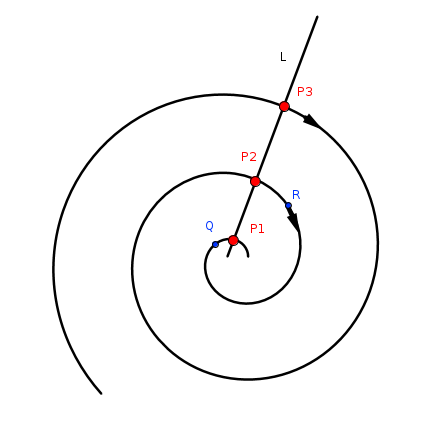
\includegraphics[width=0.5\textwidth]{transversal.png}
 	\caption{Ejemplo de transversal L.   }
 	\label{transversal}
 \end{figure}
 Usando el concepto recién definido utilizaremos cuatro lemas, que allanarán la demostración que perseguimos. Únicamente demostraremos los lemas \ref{lema1} y \ref{lema2} que son los utilizados directamente en el teorema y también son piedra angular de las pruebas de los múltiples corolarios que se pueden obtener:
 \begin{lemma}
 	\begin{enumerate}[i.]
 		\item Todo punto regular de D es un punto interior de alguna transversal, que tendrá cualquier dirección excepto la de la transversal
 		\item Toda órbita que se encuentre con una transversal debe cruzarla y todas estas órbitas la cruzarán en la misma dirección
 		\item Sea $P_0 \in D $ un punto interior de una transversal l. Para todo $\epsilon>0$ existe  un círculo $C_\epsilon$ con $P_0$ como centro tal que toda órbita que pasa por un  punto del interior de $C_\epsilon$ para $t=0$ cruza $l$ para algún $t, |t|< \epsilon$ 
 	\end{enumerate}
 \end{lemma}
 \begin{lemma}
 	Si un arco finito cerrado $A$ de una órbita C interseca una tranversal, lo hace en un conjunto finito de puntos, cuyo orden (o cantidad de puntos) en $A$ es el mismo que el orden en $l$. Si $C$ es una órbita periódica, sólo interseca a la tranversal en un punto.
 \end{lemma}
 \begin{lemma}
 	Si $C^+$ y $L(C^+)$ tienen un punto en común entonces $C^+$ es una órbita periódica.
 	\label{lema1}
 \end{lemma}
 \begin{proof} \textbf{Lema \ref{lema1}}.\\ 
 	Sea $P_1=P(t_1)$ un punto de $C^+$ que a su vez pertenezca a $L(C^+)$. Es un punto regular por lo que también es un punto interior de nuestra transversal $l$. Como $P_1 \in L(C^+)$ cualquier círculo $\Gamma$ con $P_1$ como centro, debe contener en su interior un punto $Q=P(t_k), t_k>t_1+2$. Si $\Gamma$ es el círculo para $\epsilon=1$ en el lema 2.2.3 (III), entonces existe $P_m=P(t_m)$ donde $|t_k-t_m|<1$ y $P_m$ está en $l$. Si $P_m$ es distinto de $P_1$ entonces el arco $P_1P_m$ de $C^+$ interseca a $l$ en un número finito de puntos por el lema 2.2.4. Además las intersecciones sucesivas de $C^+$ con $l$ forman una secuencia monótona que tiende a alejarse de $P_1$. Por tanto $P_1$ no puede ser un punto límite de $C^+$ (y por ende, no está en $L(C^+)$). La consecuencia es que $C^+$ solo cruza a $l$ en $P_1$, lo que implica que $C^+$ es una órbita periódica.
 \end{proof}
 \begin{lemma}
 	Si $L(C^+)$ contiene una órbita periódica entonces es idéntica a ella.
 	\label{lema2}
 \end{lemma}
 \begin{proof}\textbf{Lema \ref{lema2}}.\\
 	Sea $C_0$ una órbita periódica en $L(C^+)$ y supongamos que está contenida en $L(C^+)$. Entonces, como $L(C^+)$ es conexo, $C_0$ contiene un punto de acumulación $Q_0$ del conjunto $L(C^+)-Q_0$. Sea ahora la transversal $l$ que pasa por $Q_0$, entonces todo círculo que tenga por centro a $Q_0$ contiene un punto $Q$ de $L(C^+)-C_0$, y, para $Q$ suficientemente cercano a $Q_0$, la órbita $C_Q$ sobre $Q$ cortará a la transversal por el lema 2.2.3(III). La órbita $C_Q$, es una órbita límite por el corolario 1.1 y es distinta de $C_0$ puesto que se verifica que $C_Q\subseteq L(C^+)-C_0$. Por tanto $l$ contiene dos puntos distintos de $L(C^+)$, lo cual contradice el lema anterior. La contradicción viene de suponer que la órbita periódica está estrictamente contenida en $L(C^+)$, con lo que demostramos el resultado.
 \end{proof}
 Concluidos los lemas previos, obtenemos la demostración del teorema de Poincaré Bendixson:
 \begin{proof}
 	Claramente si $C^+$  es una órbita periódica entonces $C^+=L(C^+)$ . Por tanto asumimos de aquí en adelante que $C^+$  no es periódica. Como $L(C^+)$ no es vacío  y consiste solo en puntos regulares existe por el teorema 2.2 una órbita límite $C_0$ en $L(C^+)$. Ahora, dado que $C_0\subseteq K$, esto implica que la semiórbita $C_0^+$ tiene un punto límite $P_0$ y $P_0 \in L(C^+)$, para $L(C^+)$ cerrado. Si l es una transversal por $P_0$, entonces, dado que $P_0$ y $C_0^+$ están ambas en $L(C^+)$, la transversal l solo puede cruzar $L(C^+)$ por $P_0$ ( por el lema 2.2.3). Teniendo en cuenta que $P_0$ es un punto límite de $C_0^+$, l debe intersecar $C_0^+$ en algún punto, que debe ser $P_0$ y por tanto, $C_0^+$ y $L(C^+)$ tienen un punto en común: $P_0$. Por el lema 2.2.5 $C_0^+$ (y en consecuencia $C_0$), son órbitas periódicas, y esto implica, por el lema 2.2.6, que $C_0=L(C^+)$
 \end{proof}
 
 \begin{corollary}
 	Si $C^+$ es una semiórbita contenida en un compacto K el cual no posee puntos críticos, entonces K contiene una órbita periódica.
 \end{corollary}
 
 
 Podemos alargar el resultado un poco más, añadiendo el caso en el que nos encontremos con un número finito de puntos críticos.
 
 \begin{theorem}
 	Sea $C^+$ una semiórbita contenida en un subconjunto compacto K de D y suponiendo que D tenga un número finito de puntos críticos. Entonces se pueden dar tres situaciones (excluyentes):
 	\begin{enumerate}
 		\item $L(C^+)$ consiste en un único punto crítico de F al cual se aproxima $C^+$ cuando $t\leq \infty$,
 		\item $L(C^+)$ es una órbita periódica,
 		\item $L(C^+)$ consiste en un conjunto finito de puntos críticos de F y un conjunto de órbitas, cada una de las cuales tiende a cada uno de los puntos críticos.
 	\end{enumerate}
 \end{theorem}

\subsection{Otros criterios útiles}
Mostramos en este apartado cómo el teorema de Poincaré Bendixon es bastante singular en su campo. Tenemos frente a él multitud de criterios para eliminar la existencia de órbitas cerradas. Presentamos, para ilustrar este comentario dos ejemplos también muy útiles.
\subsubsection{Criterio de Dulac}
\begin{theorem}
	Sea $(x_1,x_2)'=f(x_1,x_2)$ un campo de vectores definido en un subconjunto conexo $R$ del plano de componentes $(f_1(x_1,x_2), f_2(x_1,x_2))$. Si existe una función real de variable real, continuamente diferenciable $g(x_1,x_2)$ tal que $\nabla(g.f)) $ tiene signo constante distinto de $0$  en $R$, entonces $R$ no puede albergar ninguna órbita cerrada completa.
\end{theorem}
\begin{proof}
Sin perder generalidad, supongamos que existe una función $g(x_1,x_2)$ de manera que \[ \frac { \partial (g.f_1) }{ \partial x_1 } +\frac { \partial (f_2.g) }{ \partial x_2 } >0, \]
en una región simplemente conexa $R$. Sea $C$ una órbita cerrada de nuestro sistema autónomo en $R$. Sea $D$ el interior de C, que sabemos que existe por el teorema de la curva de Jordan: Toda curva cerrada simple del plano divide al plano en dos componentes conexas disjuntas que tienen a la curva como frontera común. Una de estas componentes está acotada (el interior de la curva) y la otra es no acotada y se le llama exterior\footnote{Para la demostración de este teorema, consúltese: \cite{jordan}}. Entonces, aplicamos el teorema de Green: 
\begin{align}
 \iint _{ D }^{  }{ \frac { \partial (g.f_1) }{ \partial x_1 } +\frac { \partial (f_2.g) }{ \partial x_2 } dx_1dx_2 } =\oint _{ C }^{  }{\left( -g f_2dx_1+g f_1 dx_2 \right)}= \\
= \oint _{ C }^{  }{ g \left( - x_2' dx_1+x_1' dx_2 \right)  }.
\end{align}
Pero en $C$ $dx_1=x_1'dt$ y $dx_2=x_2'dt$ por lo que la integral (2.3) es $0$. Con ello llegamos a contradicción puesto que en la primera integral de (2.2), $D$ es un área no nula y el integrando es una función cuyo signo no cambia. Esto implica que esa integral no podría ser 0, lo que nos lleva a contradicción. Por tanto no puede existir esta órbita cerrada $C$. 
\end{proof}
Más información sobre la prueba y corolarios se pueden encontrar en \cite{dulac}.

\subsubsection{Criterio del gradiente}
Decimos que nuestro sistema es un sistema conservativo o gradiente si puede ser escrito de la forma:
\begin{equation}
x'=-\nabla V.
\label{gradiente}
\end{equation}
donde V es una función escalar continuamente diferenciable llamada potencial.
\begin{theorem}
En sistemas conservativos no pueden existir órbitas cerradas.
\end{theorem}
\begin{proof}
	Supongamos lo contrario. Obtendremos contradicción considerando la evolución de V a lo largo de un ciclo de periodo $T$. 
	Por una parte, tenemos que $V(T)-V(0)=0$ por hipótesis. Pero, por otra parte
	\[ V(T)-V(0)=\int_{0}^{T}\frac{dV}{dt}dt=
	\int_{0}^{T}\nabla V\cdot x'dt=
	\int_{0}^{T}-||x'^2||<0. \]
	(Obviamos el caso $x'=0$ pues en ese caso tendríamos un punto fijo, no una órbita). Llegamos por tanto a contradicción, no pueden existir órbitas cerradas.
\end{proof}


\section{Osciladores fisiológicos}
Para mostrar una aplicación directa del teorema de Poincaré Bendixson, vamos a tratar un modelo conocido como oscilador de \textit{ Van der Pol}.

Si bien el nombre es puramente intuitivo, a modo de aclaración, estamos ante la descripción de un sistema que experimenta o es capaz de crear perturbaciones o cambios periódicos en un medio.
Este oscilador fue descrito originalmente por Balthasar Van der Pol \cite{vander} debido al descubrimiento de lo que el denominó \textit{oscilaciones de relajación}, en circuitos que usaban válvulas de vacío. Pudiera parecer que estamos ante un nuevo concepto, pero estas oscilaciones corresponden a nuestra definición de conjuntos límite, matizando que nos referimos al caso de órbitas cerradas.

Aunque la aparición de este concepto está alejada de ámbitos biológicos, no tardaron en aparecer aplicaciones al campo de la neurociencia. La primera de ellas corresponde a los trabajos de Fithugh y Nagumo donde aplicaron el modelo sobre un campo bidimensional para describir el potencial de acción de las neuronas \cite{fit, nagu}. No sólo la neurociencia se vio alumbrada bajo este nuevo modelo, en \cite{mathmobi} podemos encontrar como esas ecuaciones también se usaron para describir otros procesos fisiológicos como las oscilaciones de los latidos del corazón.

\begin{equation}
x''-\alpha(1-x^2)x'+x=0,\text{ } (\alpha>0).
\label{vanderpol}
\end{equation}

En estas condiciones, fijando el parámetro como $\alpha=1$ vamos a realizar un cambio de variable para disponer del sistema de una forma más operable:
\begin{equation}
y=x-\frac{x^3}{3}-\frac{x'}{1}.
\label{cambio}
\end{equation}
De donde:
\begin{equation}
x'=(x-\frac{x^3}{3}-y).
\end{equation}
Derivo (\ref{cambio}), 
\begin{equation}
y'=x'(1-x^2)-\frac{x''}{1}.
\label{77}
\end{equation}
De (\ref{vanderpol}) tenemos:
\begin{equation}
\frac{x}{1}=-\frac{x''}{1}+(1-x^2)x'
\label{99}
\end{equation}
Igualando (\ref{77}) y (\ref{99}) nos queda esta representación:
\begin{equation}
 \left \{ \begin{matrix}x'=-y-x^3/3+x  \\y'=x\end{matrix}\right.. 
\label{vanderpol2}
\end{equation}
Acto seguido calculamos las nulclina de nuestro sistema, que igualando a $0$ cada una de las ecuaciones nos llevan a afirmar que estas vienen dadas por las curvas:
\begin{equation}
 \left \{ \begin{matrix}y=x^3/3+x \text{ (la nulclina asociada a x)}  \\x=0 \text{ ( la nulclina asociada a y)}\end{matrix}\right.. 
\label{nulclinas}
\end{equation}
Sale aquí de manifiesto el porqué este problema también es conocido como el de la nulclina cúbica. De hecho, como veremos en el comportamiento cualitativo, todas las características de nuestro modelo sencillo nos llevan indudablemente a una rápida aplicación del teorema.
De (\ref{nulclinas}) podemos observar el siguiente comportamiento de los vectores de dirección de nuestras soluciones, teniendo en cuenta (\ref{vanderpol2}):
\begin{figure}[h]
	\centering
	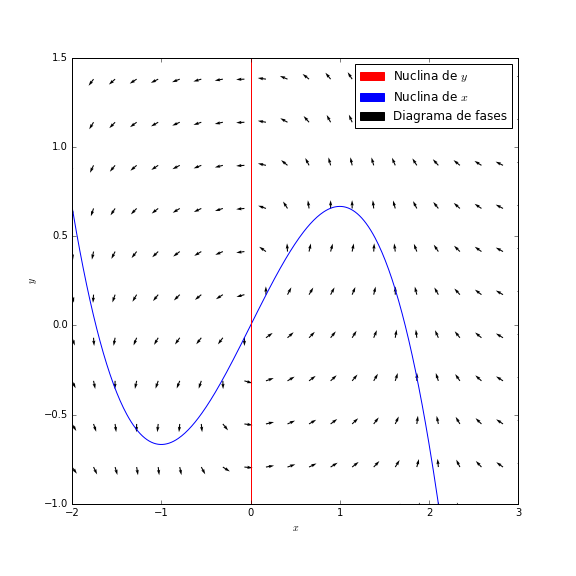
\includegraphics[width=0.5\textwidth]{phasefinal.png}
	\caption{Diagrama de fase de nuestro oscilador. Se puede observar la aparición del ciclo límite  }
\label{poincaa}
\end{figure}
\begin{itemize}
	\item La dirección debe ser \textquotedblleft vertical\textquotedblright en la nulclina de $x$ y \textquotedblleft horizontal\textquotedblright en la de $y$ (ya que $x' = 0$ o $y' = 0$, respectivamente).
	\item Cuando x es positivo, $y$ disminuye.
	\item  En la nulclina de $y$, $x$ es cero de modo que $x^3/3-x$ es también cero. Así por (\ref{vanderpol2}) $x'=y$, y $x$ aumentará cuando $y$ sea positiva y disminuirá cuando $y$ sea negativa.
\end{itemize}
Consideremos ahora una trayectoria que emana de un punto arbitrario en el primer cuadrante (el positivo). El flujo en la proximidad del nulclina de $x$ lo llevará a través de una disminución de valores de $x$. Después de llegar al segundo cuadrante y cerca del mínimo local de la nulclina, el flujo se desvía horizontalmente a través de y, hacia la rama izquierda de la curva cúbica.
Aquí una corriente en la dirección y positiva llevaría la solución desde el tercer cuadrante, de nuevo al primero como se observa en la Figura (\ref{vande}).\\
\begin{figure}[h]
	\centering
	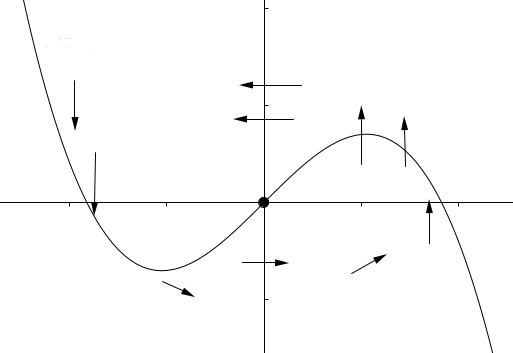
\includegraphics[width=0.5\textwidth]{vande.png}
	\caption{Diagrama de los vectores alrededor de la nulclina según el estudio.  }
	\label{vande}
\end{figure}

Concluida esta observación es evidente, además, que la solución permanecerá dentro o paralela a una región acotada, indicando que una vez que una trayectoria ha entrado en la región, está atrapada para siempre. 

En esta región además, hay un punto fijo: $(0,0)$.
Si calculamos la matriz Jacobiana para estudiar su estabilidad, obtenemos:
\[ J= \begin{pmatrix} 1-x^2 & -1 \\ 1 & 0 \end{pmatrix} .\]
Por lo que evaluando en $(0,0)$ obtenemos $Traza(J(0,0))=1$ y $Det(J(0,0))=1$. Tenemos espirales que repelen, es decir, un punto inestable.\\
Por lo tanto podemos aplicar el teorema de Poincaré-Bendixson concluyendo que hay un ciclo límite dentro de esta región. \\
Este oscilador ha sido además utilizado en otras áreas como la neurociencia. Ayudándose del mismo Tizhugh y Nagumo (como se puede ver en \cite{mathmobi}), aplicaron los conceptos subyacentes para estudiar el potencial acción de las neuronas.

En análisis de posteriores casos de este trabajo, se usará también este teorema para detectar la existencia de órbitas periódicas.
 
 
 
 \section{Conceptos Básicos de teoría de Bifurcaciones}
 La teoría de bifurcaciones es una rama de estudio relativamente reciente. Adquiere verdadera importancia  a partir de un artículo famoso de E.Hopf publicado en 1942, donde se relaciona la aparición de soluciones periódicas con ciertos cambios en el comportamiento de la parte lineal del sistema tras un cambio de un parámetro.\\
 Antes de formalizar el concepto, nos adentramos en esta teoría a través de una definición que, si bien no es estrictamente rigurosa, nos sirve para captar el concepto rápidamente gracias a nuestros conocimientos acerca de la noción de estabilidad que obtenemos en la asignatura Ecuaciones Diferenciales II: 
 \begin{defi}[Bifurcación (Intuitiva)]
 	Una bifurcación en un sistema dinámico no es mas que un cambio cualitativo en el diagrama de fases de nuestro sistema originado por la variación de uno o varios de los parámetros que en él se encuentran (mas concretamente cuando este parámetro alcanza o sobrepasa un valor crítico).
 \end{defi}
 Entendida la idea intuitiva pasamos a formalizar el concepto. He querido partir de una base sólida para no dar por sentado aspectos que pudieran pasarse por alto. Es por eso que comienzo desde la raíz topológica de esta rama.
 Si queremos estudiar las diferencias entre características cualitativas de los sistemas dinámicos, debemos razonar que este estudio pasará inexorablemente por clasificar los tipos de comportamientos que podemos observar en nuestros sistemas y compararlos entre sí. Para ello se hace indispensable la creación de una relación de equivalencia rigurosamente definida que nos permita decidir cuando dos sistemas dinámicos (o un conjunto de $n \in \mathbb{N}$ ) son cualitativamente similares o equivalentes:
 \begin{defi}[Equivalencia topológica entre dos sistemas dinámicos]
 	Un sistema dinámico $ \{T, \mathbb{R}^n , \phi(t) \}$ es considerado topológicamente equivalente o equivalente a un sistema dinámico $ \{T, \mathbb{R}^n , \psi(t) \}$ si existe un homeomorfismo $h : \mathbb{R}^n \rightarrow \mathbb{R}^n$ que lleva las órbitas del primero en las de el segundo, preservando la dirección del tiempo.
 	\label{topequi}
 \end{defi}
 Entiéndase que $T$ puede ser una variable temporal tanto continua como discreta. Además podemos considerar otros espacios de $\mathbb{R}^n$ para los que nuestra definición también sería correcta y útil, por ejemplo el toro o la esfera.
 Sin embargo, dado que la mayoría de modelos a estudiar estarán planteados en $\mathbb{R}$ o $\mathbb{R}^2$ , trabajaremos con ellos, de aquí en adelante.
 Tenemos ya todas las herramientas para definir correctamente el objeto de nuestro estudio: \\
 
 Sea el sistema dinámico definido por: 
 \begin{equation}
 x'=f(x,\alpha)
 \label{defi1}
 \end{equation}
 donde $x \in \mathbb{R}^n$ corresponde a nuestras variables y $\alpha \in \mathbb{R}^n$ corresponde a los parámetros que aparecen en nuestro sistema.
 \begin{defi}[Bifurcación (formal)]
 	La aparición de un diagrama de fases de \ref{defi1} no equivalente topológicamente bajo la variación de $\alpha$ es lo que denominamos bifurcación.
 \end{defi}
 
 Antes de pasar a la clasificación de una variada cantidad de bifurcaciones nos queda definir una forma estándar, no tanto un representante de cada una de las clases de equivalencia, si no más bien una forma de encontrar a éste:
 
 \begin{defi}[Forma Normal]
 	Diremos que un sistema de la forma: 
 	\begin{equation}
 	\xi'=f(\xi,\beta)
 	\end{equation}
 	donde $f$ es de forma polinomial con un punto de equilibro en $\xi=0$ cuando $\alpha=0$, es la forma normal de \ref{defi1} si son localmente topológicamente equivalentes en un entorno del equilibrio cuando $x=0$ y $\alpha=0$.
 \end{defi}
 
 Y, por último, durante nuestro estudio utilizaremos una representación visual de las bifurcaciones, lo que conocemos por un diagrama de bifurcaciones:
 \begin{defi}[Diagrama de Bifurcaciones]
 	Un diagrama de bifurcaciones de $(2.1)$ no es mas que una representación gráfica que enfrenta a nuestra variable x con el valor de nuestro parámetros y delimita las zonas agrupando las soluciones que son topológicamente equivalentes. 
 \end{defi}
 
 \subsection{Clasificación de las principales bifurcaciones en sistemas \\  1-dimensionales y 2-dimensionales}
 
 \subsubsection{Sistemas 1-dimensionales}
 
 \begin{enumerate}
 	\item Bifurcación Saddle Node o Fold\\
 	Esta bifurcación es el mecanismo básico mediante el cual, a través de la variación del parámetro aparecen y colisionan\footnote{el término colisión no es casual, basta comprobar que, sea $v(\alpha)$ la velocidad de aproximación de los puntos fijos $\Rightarrow$ $v(\alpha) \rightarrow \infty $ cuando $\alpha \rightarrow 0$} puntos fijos. 
 	La forma normal de esta bifurcación es:
 	\begin{equation}
 	x'=\alpha+x^2
 	\label{sadd}
 	\end{equation}
 	donde $\alpha$ es un parámetro que puede ser positivo, negativo o 0.
 	Para estudiar de manera óptima como cambia nuestra solución discutiremos la variación en una partición de $\mathbb{R}$:\\
 
 	\begin{itemize}
 		\item $\alpha \in \mathbb{R^-} $ : en este caso el signo de la derivada cambia cuando x=0 por lo que tendremos la existencia de dos puntos fijos $x_{1,2}(\alpha)=\pm \sqrt{-\alpha}$: uno estable puesto que la derivada será positiva $\forall x \in \mathbb{R},\text{ } x < x_1$ y negativa $\forall x \in \mathbb{R},\text{ } x_1< x < x_2$. Otro inestable, puesto que los signos de la derivada varían de forma opuesta: negativa para $\forall x \in \mathbb{R},\text{ } x_1 <x < x_2$ y positiva para $\forall x \in \mathbb{R},\text{ } x_2 < x$
 	\begin{figure}[h]
 		\centering
 		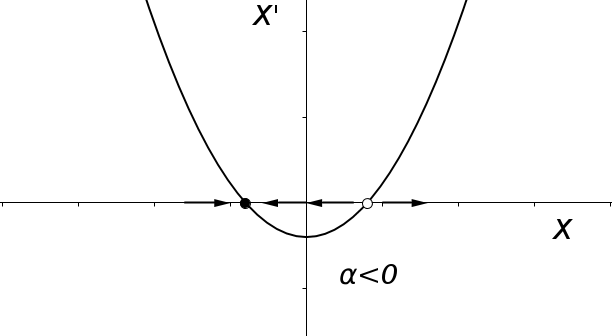
\includegraphics[width=0.5\textwidth]{saddlenode3.png}
 		\caption{Comportamiento de (\ref{sadd}) con $\alpha<0$.}
 	\end{figure}
 		\item $\alpha=0$
 		: en este caso tendremos un punto fijo en 0, estable por la izquierda e inestable por la derecha
 		\begin{figure}[h]
 			\centering
 			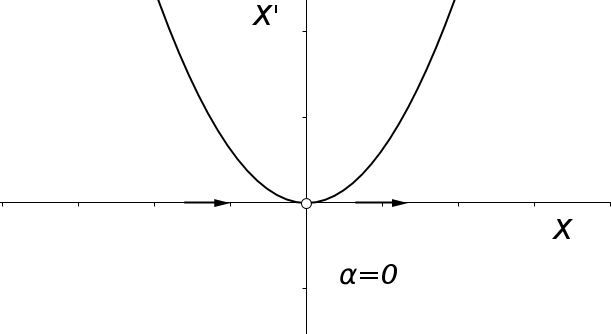
\includegraphics[width=0.5\textwidth]{saddlenode4.png}
 			\caption{Comportamiento de (\ref{sadd}) con $\alpha=0$.}
 		\end{figure}
 		\item $\alpha \in \mathbb{R^+} $ : en este caso no tenemos ningún punto fijo
 		\begin{figure}[h]
 			\centering
 			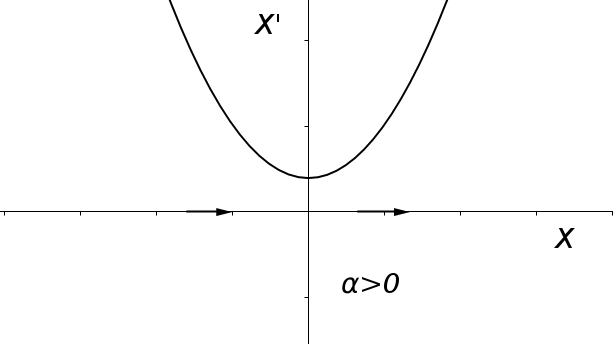
\includegraphics[width=0.5\textwidth]{saddlenode5.png}
 			\caption{Comportamiento de (\ref{sadd}) con $\alpha>0$.}
 		\end{figure}
 	\end{itemize}
 	A modo de resumen gráfico dibujaremos a continuación el diagrama de bifurcaciones de este tipo (\ref{diagfold}). Es de destacar que para comprender el gráfico basta observar que el mismo nos da información sobre la aparición y desaparición de puntos fijos y por supuesto y sobre el cambio en el diagrama de fases según $\alpha$ varía. Es por esto que $\alpha$ suele aparecer en el eje horizontal.
 	\begin{figure}[h]
 		\centering
 		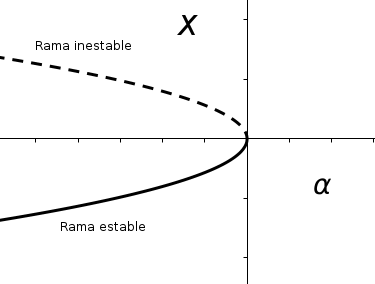
\includegraphics[width=0.5\textwidth]{saddlenodediagrama.png}
 		\caption{Diagrama de bifurcación de Saddle Node.}
 		\label{diagfold}
 	\end{figure}
 	Como veremos más adelante la bifurcación fold y la bifurcación de Hopf (que definiremos en el siguiente apartado) son de las bifurcaciones básicas más importante en biología. Esto se debe a que en el resto de bifurcaciones, bajo ligeras variaciones en los parámetros, aparecerán en nuestros diagramas zonas con un comportamiento local idéntico a la bifurcación fold. Buena prueba de ello es el tema dedicado a este fenómeno en \cite{Strogatz}. Es por eso que decidimos estudiar, a modo de ejemplo generalizable, la obtención de la forma normal de ésta.
 	
 	Para ello, basándonos en el desarrollo ejemplificado en \cite{Kuznet} o \cite{murdock}, comenzamos probando un lema sencillo que nos habla sobre la persistencia de esta bifurcación ante la introducción de nuevos términos en la expresión de $f(x,\alpha)$ lo cual nos dará vía libre para entender como tratar casos en los que aparece esta bifurcación, llegando así a su forma normal:
 	\begin{lemma}
 		Supongamos que tenemos nuestra ecuación de la forma \[ x' = {\alpha}+ x^2 .\]
 		Si añadimos a nuestra ecuación términos de orden superior\footnote{Por ejemplo: $\mathcal{O}(x^2)$ designará a expresiones  cuyo valor, cuando tiendan a infinito, quede acotado por una expresión de la forma $ax^2$, con $a$ constante } (denotados por $\mathcal{O}$) entonces el sistema de la forma:
 		\begin{equation}
 		x' = {\alpha}+ x^2 + \mathcal{O}(x^3) .
 		\label{fold3}
 		\end{equation}
 		es topológicamente equivalente en un entorno del origen a 
 		\[ x' = \alpha + x^2. \]
 		Ocurre por tanto que nuestro sistema no muestra un cambio cualitativo en su comportamiento cerca del origen.
 	\end{lemma}
\begin{proof}
	La prueba la podemos dividir en dos partes, primero analizaremos que en ambas expresiones encontramos los mismo puntos fijos (con la misma naturaleza) y luego construiremos un homeomorfismo que nos lleve de un sistema a otro. Esta prueba se fundamenta en el hecho de que para sistemas dinámicos escalares un homeomorfismo que lleve los puntos de equilibrio en puntos de equilibrio de otro sistema también hará lo propio con las órbitas.
	\begin{enumerate}
		\item Introducimos una variable escalar, de manera que nuestro sistema quede de la forma
		\[ y' = F (y, \alpha) = \alpha + y^2 + \psi(y,\alpha) .\]
		donde $ \psi = O(y^3 )$ una función de $(y,\alpha)$ continuamente diferenciable ( o $C^\infty$) en un entorno de (0, 0). Ahora, consideramos la naturaleza de la variedad que nos define el equilibrio cerca del $(0, 0)$ del plano formado por $(y,\alpha)$ :
		\[ M = \{(y,\alpha) : F (y,\alpha) = \alpha + y^2 + \psi(y,\alpha) = 0\} .\]
		En este caso podemos hablar de una curva que pasa por el origen ($F(0,0)=0$). Por el teorema de la función implícita (pues $F_\alpha(x,\alpha)=1$), admite una parametrización local como:
		\[ M = \{(y,\alpha) : \alpha = g(y)\} . \]
		con g es continuamente diferenciable y está definida para valores de $y$ cercanos a $0$. De hecho, la expresión de g nos queda
		\[ g(y) = -y^2 + \mathcal{O}(y^3) .\]
		Por tanto para pequeñas variaciones de $\alpha < 0$ tendremos comportamiento similar, es decir la existencia de dos puntos fijos cerca del origen  $y_2(\alpha), y_1(\alpha)$.
		\item Construimos ahora un homeomorfismo dependiente de $\alpha$, para valores cercanos a 0. Para valores  $\alpha \geq 0$ tomamos la aplicación identidad:
		\[ h_\alpha (x) = x .\]
		Para valores de $\alpha \textless 0$ tomamos la transformación lineal:
		\[ h_\alpha (x) = \delta (\alpha) + b(\alpha)x. \]
		donde los valores de $\delta$ y b quedan determinados por el efecto de la aplicación sobre los valores de nuestros dos puntos fijos (los de partida y los de llegada):
		\[ h_\alpha (x_j (\alpha)) = y_j(\alpha), j = 1, 2 .\]
		Tenemos por tanto un homeomorfismo $h_\alpha:\mathbb{R}^1 \to \mathbb{R}^1$, que nos lleva de unas órbitas a otras (por el resultado que señalábamos en el primer párrafo, comentado en \cite{Kuznet}), preservando la dirección del tiempo. Por tanto, por la definición de equivalencia de sistemas, tenemos el resultado.
	\end{enumerate}
\end{proof}
Este resultado nos da pie a generalizar la forma normal de la bifurcación: 
\begin{theorem}[Forma normal de la bifurcación fold]
	Supongamos el sistema 1-dimensional:
	\begin{equation}
	x'=f(x,\alpha),
	\end{equation}
	con f derivable y un punto fijo en $x=0$ cuando $a=0$. Supongamos además que verifica: $f_x(0,0)=0$, $f_{xx}(0,0) \neq 0)$ y $f_\alpha(0,0) \neq 0$ Entonces nuestro sistema tiene una bifurcación fold y su forma normal puede escribirse como: \[x'=\alpha+x^2.\]
\end{theorem}
\begin{proof}
	\textit{Skecth de la prueba}\cite{prac,Kuznet}: La idea fundamental detrás de esta demostración es, como en el lema previo, puramente constructiva. Es por ello que dejamos los pasos de la misma, aunque no profundicemos en la operaciones. 
	Dado un sistema con una función continuamente diferenciable f que posee en $\alpha=0$ un equilibrio en $x=0$ y $f_x(0,0)=0$, podemos utilizar el desarrollo en serie de Taylor para llegar a esta expresión:
	\[f(x,\alpha)=f_0(\alpha)+f_1(\alpha)x+f_2(\alpha)x^2+\mathcal{O}(x^3).  \]
	La filosofía de la prueba es, mediante cambios de variables invertibles ( y $C^\infty$) en la variable y el parámetro, transformar el sistema en uno equivalente de la forma (\ref{fold3}), y aplicar el lema demostrado.
	
	
\end{proof}


Equivalentemente podemos tratar el caso 
\begin{equation}
x'=\alpha-x^2.
\end{equation}
cuyo comportamiento es similar respecto de la variación entre $[-\infty,+\infty]$ de $\alpha$, siendo simétrico en cuanto a esquema pero permutándose las ramas estables e inestables.

Es habitual que en la clasificación de bifurcaciones no haya un consenso generalizado sobre el nombre de las mismas. Para evitar confusiones he de resaltar que esta bifurcación también recibe el nombre de bifurcación de doblez (fold bifurcation) o de punto giratorio (turning point bifurcation)


\item Bifurcación transcrita\\
Es habitual también, encontrarnos casos en los que para toda variación del parámetro encontramos existencia de puntos fijos (tanto estables como inestables). \\
Dentro de este esquema presentamos la siguiente bifurcación denominada transcrita En ella siempre, para todo valor de  $\alpha$ hallaremos la existencia  de nodos, sin embargo estos cambiarán su estabilidad.
\\
Podemos observar este comportamiento en la siguientes gráficas \ref{trans1}, \ref{trans2}, \ref{trans3}:
\begin{figure}[H]
	\centering
	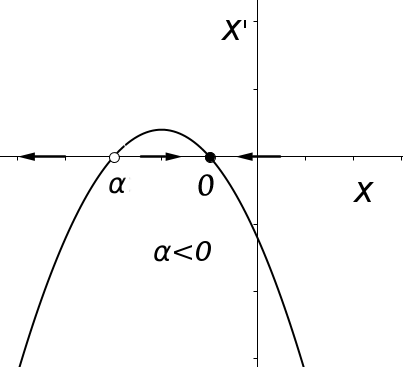
\includegraphics[width=0.45\textwidth]{trans1.png}
	\caption{Comportamiento de (\ref{trans}) en $\alpha<0$.}
	\label{trans1}
\end{figure}
\begin{figure}[H]
	\centering
	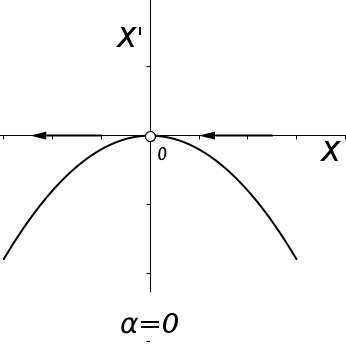
\includegraphics[width=0.45\textwidth]{trans2.png}
	\caption{Comportamiento de (\ref{trans}) en $\alpha=0$ .}
	\label{trans2}
\end{figure}
\begin{figure}[H]
	\centering
	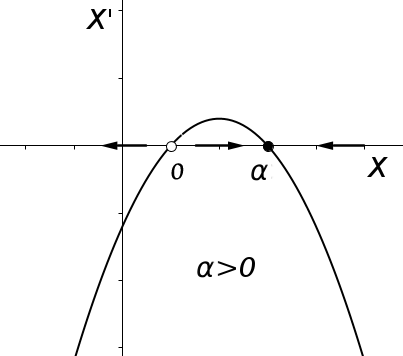
\includegraphics[width=0.45\textwidth]{trans3.png}
	\caption{Comportamiento de (\ref{trans}) en $\alpha>0$.}
	\label{trans3}
\end{figure}
Para presentar esta bifurcación recurrimos de nuevo a la forma normal:
\begin{equation}
x'=x(\alpha-x).
\label{trans}
\end{equation}
donde $\alpha$ es un parámetro que puede ser positivo, negativo o 0.
Teniendo todos los ingredientes para poder dibujar nuestro diagrama de bifurcaciones (Figura \ref{trandia}).
\begin{figure}[H]
	\centering
	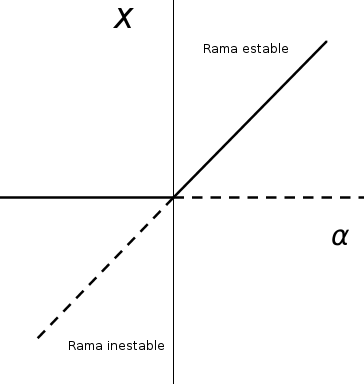
\includegraphics[width=0.5\textwidth]{trandiagrama.png}
	\caption{Diagrama de bifurcaciones de la bifurcación transcrita}
	\label{trandia}
\end{figure}

Un ejemplo trivial de este comportamiento puede verse en ecuaciones que modelizan crecimiento de poblaciones. Destacaremos su aparición en modelos epidemiológicos en los apartados de aplicaciones.


\item Bifurcación de Pitchfork

En este caso nos encontramos con una bifurcación en la cual según varía el parámetro aparecerán 3 nodos o puntos fijos (es por esto que es habitualmente llamada de tenedor o tridente). Es una bifurcación que suele aparecer en casos en los que el sistema presenta algún tipo de simetría, además también se la suele denotar biestable, debido a la aparición de las dos ramas estables cuando el parámetro crece.

Dentro de este tipo de bifurcaciones encontramos dos casos bien diferenciados:
\begin{enumerate}
	\item Bifurcación de pitchfork supercrítica
	
	La primera bifurcación de este tipo que presentamos, es la supercrítica. Recogemos aquí su forma normal de la cual comenzaremos a deducir propiedades:
	\begin{equation}
	x'=\alpha x-x^3=x(\alpha-x^2).
	\label{pitch}
	\end{equation}
	donde $\alpha$ es un parámetro que puede ser positivo, negativo o 0.
	Vemos desde un primer momento que esta función es invariante para cambios de variables del tipo: $x \rightarrow -x$. Más formalmente diremos que en este caso el campo de vectores es equivariante, es decir, que el resultado de aplicar una simetría a la función y luego representarla es lo mismo que representar la función en nuestro dominio y luego realizar la simetría.
	Vamos con la representación: \\
	\begin{figure}[H]
		\centering
		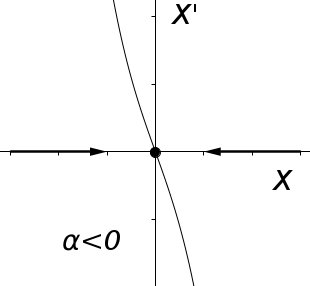
\includegraphics[width=0.45\textwidth]{pitch11.png}
		\caption{Comportamiento de (\ref{pitch}) en $\alpha<0$. }
	\end{figure}
	\begin{figure}[H]
		\centering
		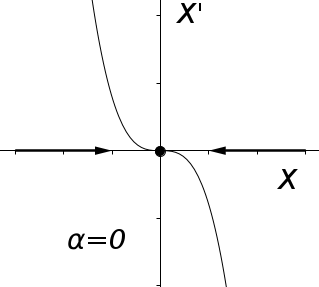
\includegraphics[width=0.45\textwidth]{picth12.png}
		\caption{Comportamiento de (\ref{pitch}) en $\alpha=0$ .}
	\end{figure}
	\begin{figure}[H]
		\centering
		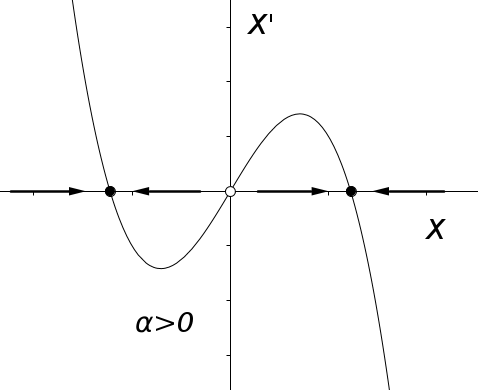
\includegraphics[width=0.45\textwidth]{picth13.png}
		\caption{Comportamiento de (\ref{pitch}) en $\alpha>0$. }
	\end{figure}
	Como podemos observar en los gráficos, cuando $\alpha$ es menor que 0 o estrictamente igual a cero siempre tenemos un punto fijo, estable en $x=0$. Sin embargo conforme nuestro parámetro tiende  cero podemos observar visualmente como \textquotedblleft la estabilidad se va haciendo cada vez más débil\textquotedblright  hasta terminar por desaparecer en 0 cuando $\alpha \textgreater 0$. Al mismo tiempo cuando esto sucede se crean dos puntos fijos estables.
	
	Una vez concluido este estudio podemos representar trivialmente el diagrama de bifurcaciones, del cual se puede comprender mejor la denotación de esta bifurcación (Figura \ref{pitch1}).\\
		\begin{figure}[H]
			\centering
			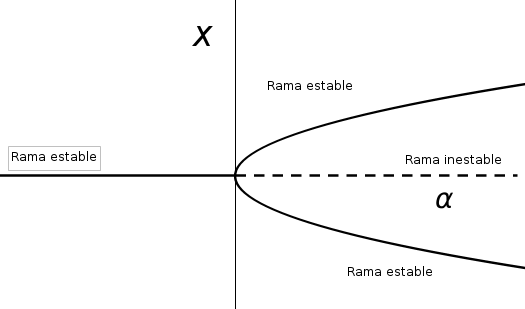
\includegraphics[width=0.5\textwidth]{pitch1diagrama.png}
			\caption{Diagrama de bifurcaciones pitchfork supercrítica.}
			\label{pitch1}
		\end{figure}
	
	\item Bifurcación de pitchfork subcrítica\\
	Discutimos ahora el siguiente caso de bifurcación tipo pitchfork: subcrítico En esta bifurcación nos encontramos ante un comportamiento de tridente gráficamente similar a nuestro anterior estudio pero en este caso predominarán los nodos inestables. Representamos a continuación el aspecto local que tienen las bifurcaciones de este tipo: 
	la forma normal de esta bifurcación es la siguiente:
	\begin{equation}
	x'=\alpha x+x^3=x(\alpha +x^2)
	\label{pitch2}
	\end{equation}
	donde $\alpha$ es un parámetro que puede ser positivo, negativo o 0.\\
	Como podemos observar la evolución de nuestro sistema según varía $\alpha$ es muy similar al caso anterior. \\Si $\alpha \textless 0$ encontraremos 2 puntos de equilibrio, dos inestables y unos estable en 0. Cuando $\alpha \geq 0$ los puntos de equilibrio confluyen en 0, quedando un solo punto fijo inestable.
	Con esta información podemos elaborar ya el diagrama de bifurcaciones \ref{pitch21}
	\begin{figure}[H]
		\centering
		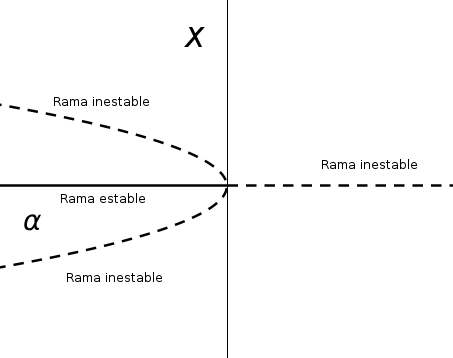
\includegraphics[width=0.5\textwidth]{pitch2diagrama.png}
		\caption{Diagrama de bifurcaciones Pitchfork subcrítica}
		\label{pitch21}
	\end{figure}
\end{enumerate}
Concluimos con esto la introducción para bifurcaciones 1-dimensionales.


 Evolucionando de estas obtendremos algunas de la bifurcaciones usuales en 2 dimensiones. Como dije al principio este estudio no es mas que una ligera pincelada de los muchos comportamientos que podemos encontrar en nuestros sistemas dinámicos.
\end{enumerate}

\subsubsection{Sistemas 2-dimensionales}
Siguiendo la filosofía del apartado inmediatamente anterior, introduciremos en este un conjunto de las bifurcaciones 2-dimensionales, que, si bien no es exhaustivo, pretende aportar una idea general, la cual, combinada con nuestros conocimientos de estabilidad de Ecuaciones Diferenciales II, nos puede dar pie a profundizar cuanto queramos. \\
Es de resaltar que en sistemas dos dimensionales nos vamos a encontrar con comportamientos similares a los que se pueden observar en una dimensión. Sin embargo en este apartado no sólo los puntos fijos se verán afectados, \textquotedblleft creándose\textquotedblright o \textquotedblleft destruyéndose\textquotedblright, sino que también lo harán las órbitas cerradas.\\
Es obvio que las bifurcaciones presentadas anteriormente tienen su análogo en 2 dimensiones, por ello, presentaremos su diagrama y su forma normal, recayendo la importancia central de este apartado en la bifurcación más representativa, no vista hasta ahora. Las gráficas mostradas en relación con las bifurcaciones saddle-node, transcrítica y fold, para mejorar su comprensión, serán los diagramas de fase con la representación de sus puntos fijos y la estabilidad de los mismos.
\begin{enumerate}
	\item Bifurcación Saddle-Node. \\
	En este como en el resto de los casos, el comportamiento a estudiar no cambia, pues está restringido a una sola dimensión. Por ello añadir más dimensiones nos muestra simplemente la forma en la que las órbitas se relacionan con este subespacio, tanto si son repelidas como atraídas.
	Dado que nuestra segunda variable no dependerá de nuestro parámetro, una vez tengamos la forma normal de la variable dependiente, para completar utilizaremos una función, que simplifique nuestros cálculos. En este caso hemos escogido una exponencial:
	\begin{equation}
	\left \{ \begin{matrix}x'=\alpha+x^2, \\y'=-y.\end{matrix}\right.
	\label{fold2d}
	\end{equation}  
	
	Encontramos por tanto el mismo comportamiento en la variable $x$ (de hecho todas las bifurcaciones de Saddle Node se comportan localmente igual), únicamente influenciado por su relación con la variable $y$ que modifica el espacio de fase.
	\begin{figure}[H]
		\centering
		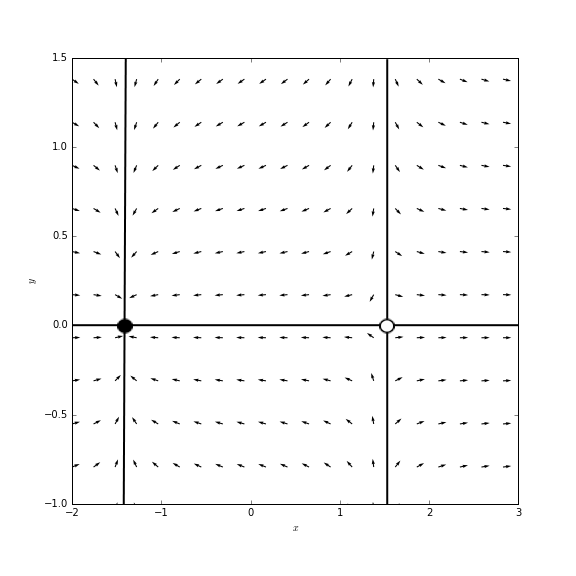
\includegraphics[width=0.45\textwidth]{fold11.png}
		\caption{Comportamiento de (\ref{fold2d}) en $\alpha<0$. }
	\end{figure}
	\begin{figure}[H]
		\centering
		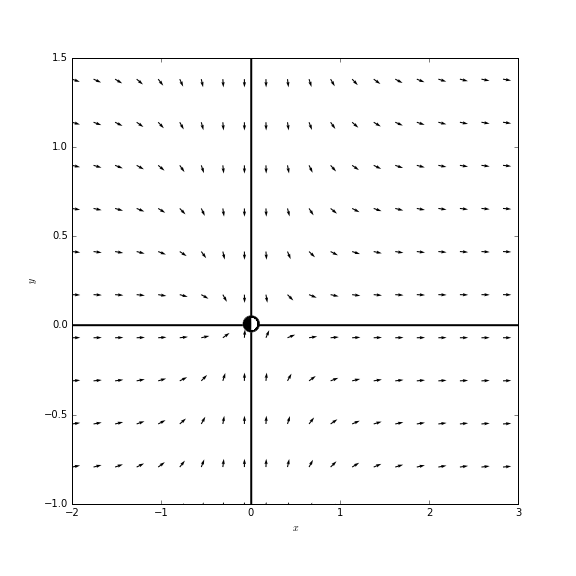
\includegraphics[width=0.45\textwidth]{fold12.png}
		\caption{Comportamiento de (\ref{fold2d}) en $\alpha=0$ .}
	\end{figure}
	\begin{figure}[H]
		\centering
		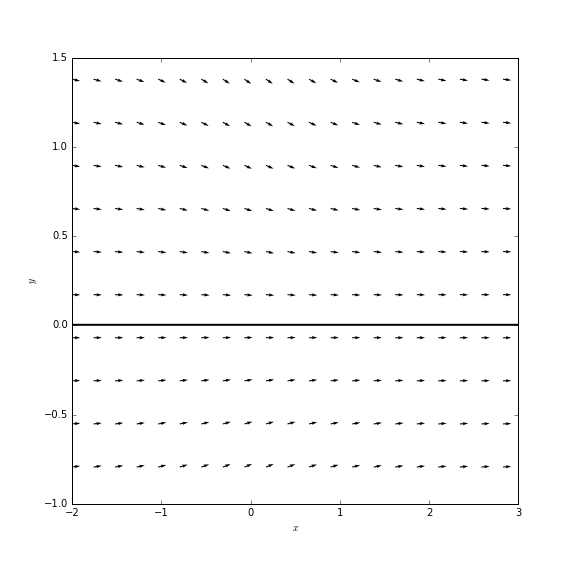
\includegraphics[width=0.45\textwidth]{fold13.png}
		\caption{Comportamiento de (\ref{fold2d}) en $\alpha>0$. }
	\end{figure}
	\item Bifurcación transcrítica. \\
	Nos encontraremos en este apartado con la forma general:
	\begin{equation}
	\left \{ \begin{matrix}x'=\alpha x-x^2 \\y'=-y\end{matrix}\right .. 
	\label{trans2d}
	\end{equation}
	Tenemos por tanto el mismo comportamiento en la variable $x$, que podemos reflejar gráficamente en los diagramas de fase. 
	\begin{figure}[H]
		\centering
		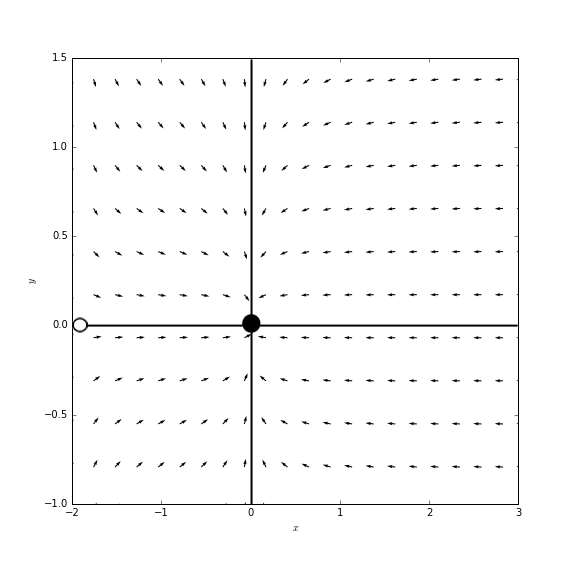
\includegraphics[width=0.45\textwidth]{trans11.png}
		\caption{Comportamiento de (\ref{trans2d}) en $\alpha<0$. }
	\end{figure}
	\begin{figure}[H]
		\centering
		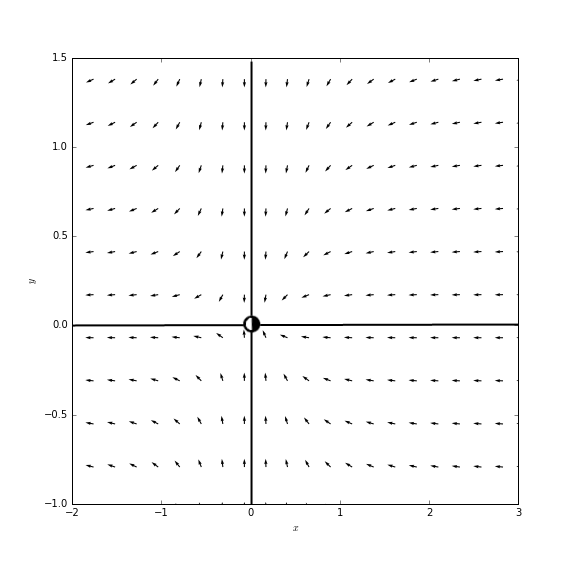
\includegraphics[width=0.45\textwidth]{trans12.png}
		\caption{Comportamiento de (\ref{trans2d}) en $\alpha=0$ .}
	\end{figure}
	\begin{figure}[H]
		\centering
		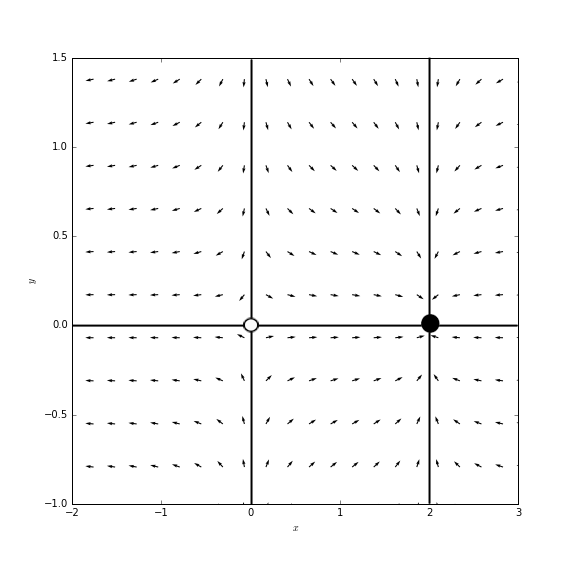
\includegraphics[width=0.45\textwidth]{trans13.png}
		\caption{Comportamiento de (\ref{trans2d}) en $\alpha>0$. } 
	\end{figure}
	\item Bifurcación Pitchfork. \\
	Juntamos en este apartado los dos tipos de bifurcación Pitchfork:
	\begin{equation}
	\left\{\begin{matrix}x'=\alpha x-x^3 \\y'=-y\end{matrix}\right..
	\label{pitch2d}
	\end{equation}
	Y la subcrítica:
	\begin{equation}
	\left\{\begin{matrix}x'=\alpha x+x^3 \\y'=-y\end{matrix}\right..
	\end{equation}
	Incluimos a modo de ejemplo, los diagramas del caso supercrítico.
	\begin{figure}[H]
		\centering
		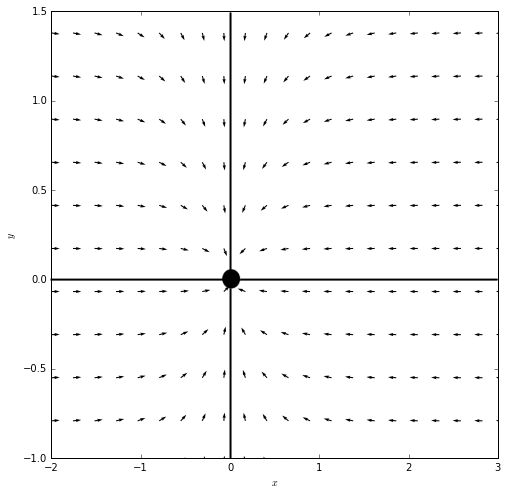
\includegraphics[width=0.45\textwidth]{pitch1.png}
		\caption{Comportamiento de (\ref{pitch2d}) en $\alpha<0$. }
	\end{figure}
	\begin{figure}[H]
		\centering
		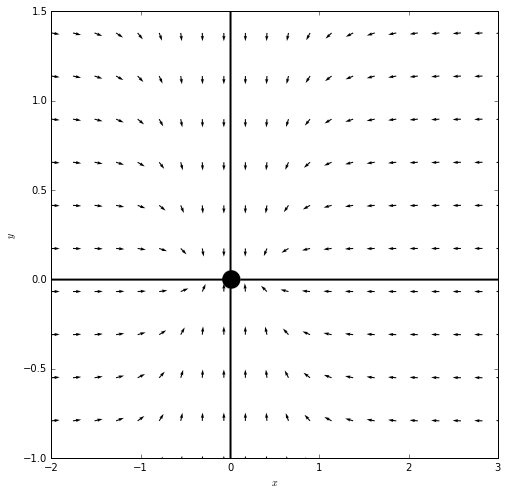
\includegraphics[width=0.45\textwidth]{pitch2.png}
		\caption{Comportamiento de (\ref{pitch2d}) en $\alpha=0$ .}
	\end{figure}
	\begin{figure}[H]
		\centering
		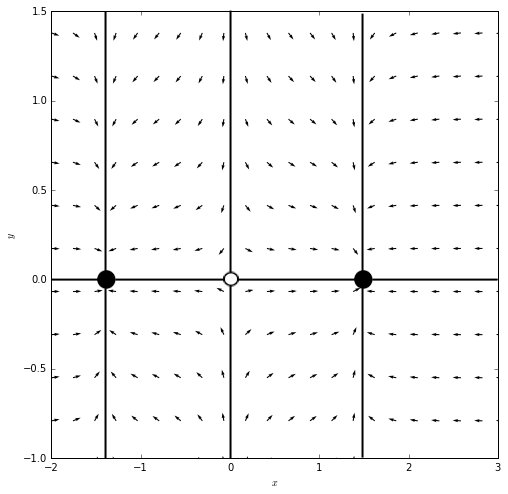
\includegraphics[width=0.45\textwidth]{pitch3.png}
		\caption{Comportamiento de (\ref{pitch2d}) en $\alpha>0$. }
	\end{figure}
	
	\item Bifurcación de Hopf o de Andronov-Hopf
	
	Hasta ahora no hemos hecho mas que extender a dos dimensiones las bifurcaciones que obteníamos en una dimensión. Esto es así por el propio carácter de los puntos fijos que estábamos considerando. Sin embargo, dado que estamos en dimensión 2, un punto fijo puede perder o modificar su estabilidad de más formas. 
	
	 Para comprender esto basta tener en cuenta como varían los valores propios del Jacobiano asociado a un sistema dinámico. Si un punto es estable los valores propios deben encontrarse en el subespacio $\Re \leq0$ (parte real menor que 0). Para que esta estabilidad cambie uno  ambos valores propios deben cruzar el eje imaginario, lo que nos ocasionará trabajar con la existencia de ciclos límite y órbitas cerradas.
	 
	Dada la importancia de esta bifurcación procederemos a estudiarla como lo hicimos con la de Saddle Node, obteniendo no solo su comportamiento sino también su forma normal. Antes de comenzar la deducción, es de destacar que al igual que en el caso de la bifurcación Pitchfork, tendremos dos tipos de bifurcación de Hopf: sub y supercrítica.\\
	Consideremos el siguiente sistema dinámico de dos variables:
	 \[ \left \{ \begin{matrix} x_1'=\alpha x_1-x_2-x_1(x_2^2+x_1^2)\\ x_2'=x_1+\alpha x_2-x_2(x_2^2+x_1^2)\end{matrix}\right.. \]
	Comprobamos que el sistema tiene puntos de equilibrio en $ x_1=0, x_2=0$:
	\begin{equation}
	\begin{split}
	&0=\alpha x_1-x_2-x_1(x_2^2+x_1^2) \\&
	0=x_1+\alpha x_2-x_2(x_2^2+x_1^2)\end{split} 
	\end{equation}
	
	
	 y, el jacobiano asociado será (tomando la parte lineal): 	 
	 \[ A= \begin{pmatrix} \alpha & -1 \\ 1 & \alpha \end{pmatrix} .\]
	cuyos valores propios serán $\lambda_{1,2} = \alpha \pm i$.
	Para estudiar el comportamiento cualitativo del sistema de forma más sencilla, dado que esto requerirá estudiar órbitas cerradas, introduciremos la variable $z$ la cual no es mas que la representación de las dos coordenadas de partida a través de un número complejo.\\
	\begin{equation}
	\begin{split}
	&z = x_1+ix_2, \\&\overline{z} = x_1-ix_2, \\ &|z|^2=z.\overline{z} = x_1^2+x_2^2.
	\end{split} 
	\end{equation}
	Esta variable satisface la ecuación diferencial,
	\[ z' = x_1' + ix_2' = \alpha(x_1 + ix_2 ) + i(x_1 + ix_2 ) - (x_1 + ix_2 )(x_1^2 + x_2^2 ). \] 
	con lo que podemos reescribir nuestro sistema inicial como: 
	\begin{equation}
	z' = (\alpha+i)z-z|z|^2 .
	\end{equation}
	Si ahora usamos el cambio de variable $z=\rho e^{i\psi}$ obtenemos, derivando:
	\[ \rho' e^{i\psi}+ i\rho\psi' e^{i\psi} = \rho e^{i\psi}(\alpha+i-\rho^2). \]
	lo cual, teniendo en cuenta el significado de la exponencial de un complejo visto en la asignatura de Variable Compleja I (fórmula de Euler), podemos traducir nuestro sistema a un sistema en coordenadas polares, el cual al estar desacoplado nos permite estudiar lo cambios cualitativos de nuestro sistema de partida según cambia el parámetro: 
	\[ \left \{ \begin{matrix} \rho' = \rho(\alpha - \rho ^2 ),\\ \psi' =1. \end{matrix}\right. \]	
	A través de esta expresión podemos deducir que $\rho$ =0 será siempre un punto de equilibrio, sin embargo su estabilidad cambiará:
	\begin{itemize}
		\item Si $ \alpha<0 $ el punto será estable (linealmente), por lo que la órbita tenderá al punto
		\item Si $\alpha=0$ el punto será estable pero no atractor, por lo que la distancia entre la solución y el punto no tiene por que disminuir exponencialmente.
		\item Si $\alpha>0$ tenemos que la estabilidad del punto cambia, para ser inestable. Sin embargo aparece una órbita cerrada, límite de todas las trayectorias en ambas componentes en $\sqrt{\alpha}$ 
	\end{itemize}
	\begin{figure}[H]
		\centering
		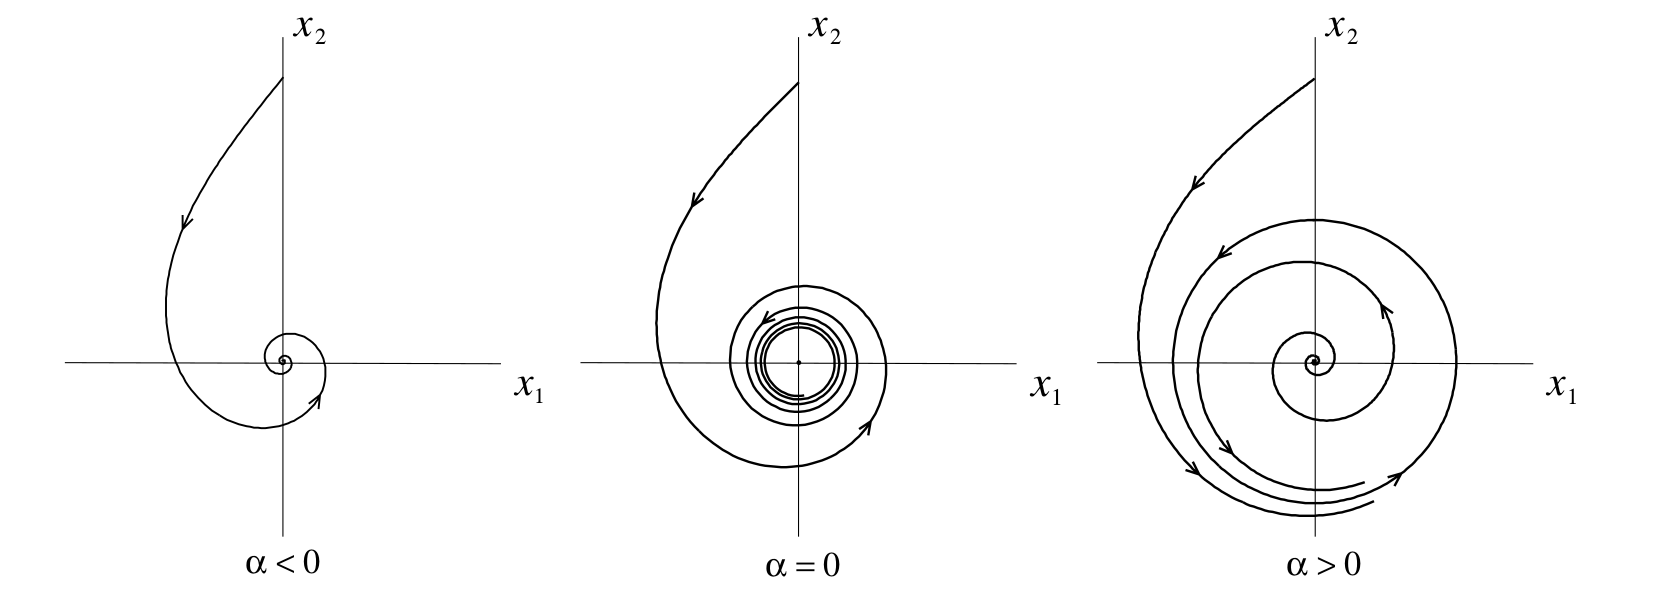
\includegraphics[width=\textwidth]{hopf11.png}
		\caption{Comportamiento Hopf supercrítica \cite{Kuznet}.}
		\label{hopf1}
	\end{figure}
	Como antes, toda esta información la podremos representar en un diagrama que nos muestre las relaciones entre x e y en varios estados de $\alpha$ o, preferiblemente, aunque quizás mas obtuso para la vista del profano, a través de un diagrama de bifurcaciones que si queremos que contenga ambas variables, será tridimensional\footnote{Veremos sin embargo, que representar tridimensionalmente diagramas de bifurcaciones suele omitirse por su costo computacional, desarrollando la mayoría de programas un gráfico que contiene toda esta información pero representable en 2 dimensiones}.
	
	Acabamos de describir la bifurcación de Hopf Supercrítica. Como avanzábamos, existe también la Hopf subcrítica:\[ \left \{ \begin{matrix} x'=\alpha x-y+x(y^2+x^2)\\ y'=x+\alpha y+y(y^2+x^2)\end{matrix}\right . .\]
	la cual, tras un cambio análogo, puede ser descrita como sigue:\[ \left \{\begin{matrix} \rho' = \rho(\alpha + \rho ^2 ),\\ \psi' =1 \end{matrix}\right .. \]
	Evidentemente encontramos un cambio notable en el comportamiento de las soluciones:
	\begin{itemize}
		\item Si $\alpha<0$ el punto 0 será un punto de equilibro estable, pero encontraremos una órbita límite inestable de radio $\sqrt{|\alpha|}$
		\item Si $\alpha=0$ La órbita límite desaparece, aunque el origen conserva la estabilidad.  
		\item Si $\alpha>0$ el punto será inestable, y con una velocidad de repulsión exponencial.
	\end{itemize}
		\begin{figure}[H]
			\centering
			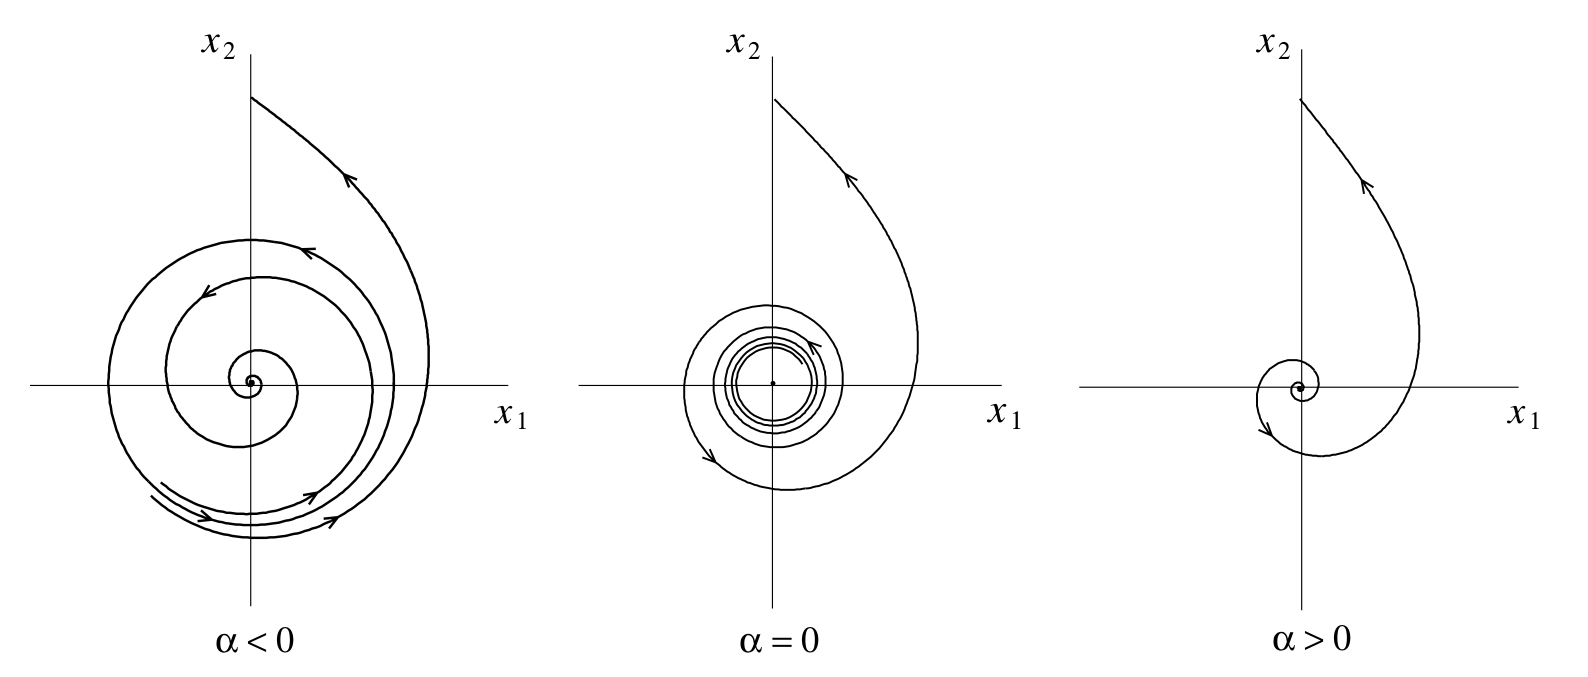
\includegraphics[width=\textwidth]{hopf21.png}
			\caption{Comportamiento Hopf subcrítica \cite{Kuznet}. }
		\label{hopf2}
	\end{figure}
	
	Presentamos de nuevo, para aclaración los diagramas de bifurcaciones. En este caso serán más difíciles de visualizar puesto que al tener un sistema 2-dimensional, la representación completa del diagrama es 3-dimensional.

\begin{figure}[H]
	\centering
	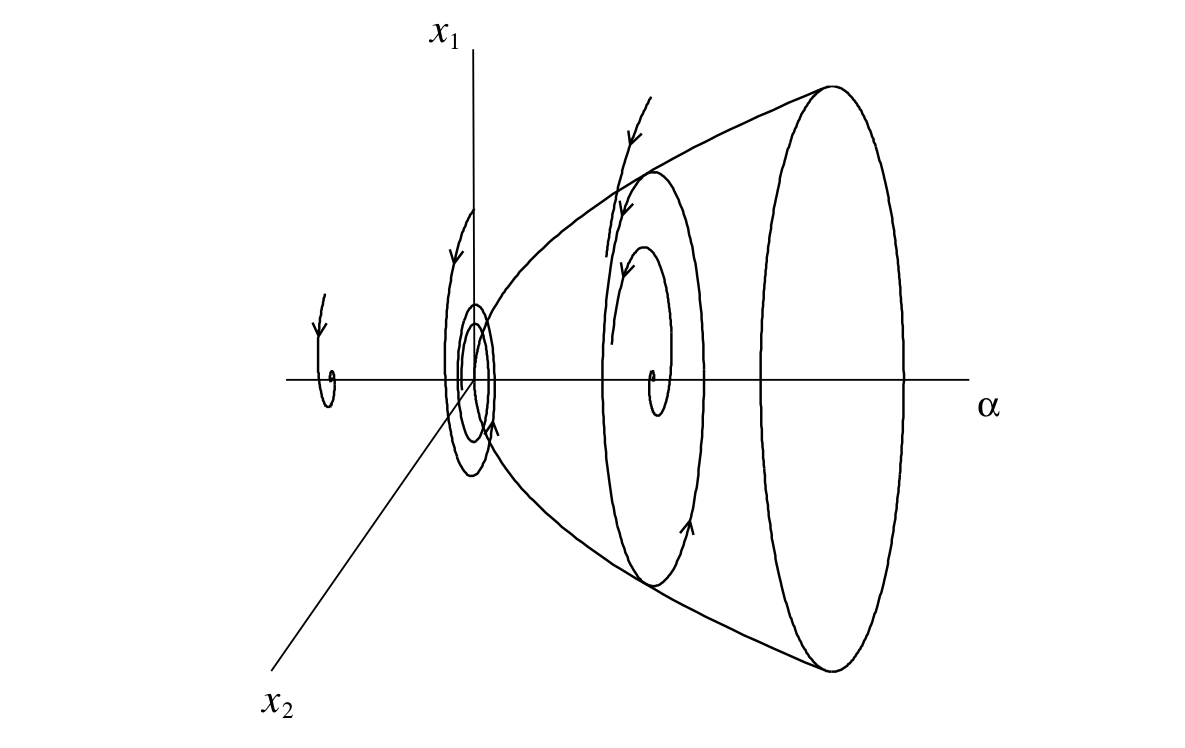
\includegraphics[width=\textwidth]{hopf12.png}
	\caption{Diagrama de bifurcaciones Hopf supercrítica\cite{Kuznet}. }
\label{hopf3}
\end{figure}
\begin{figure}[H]
	\centering
	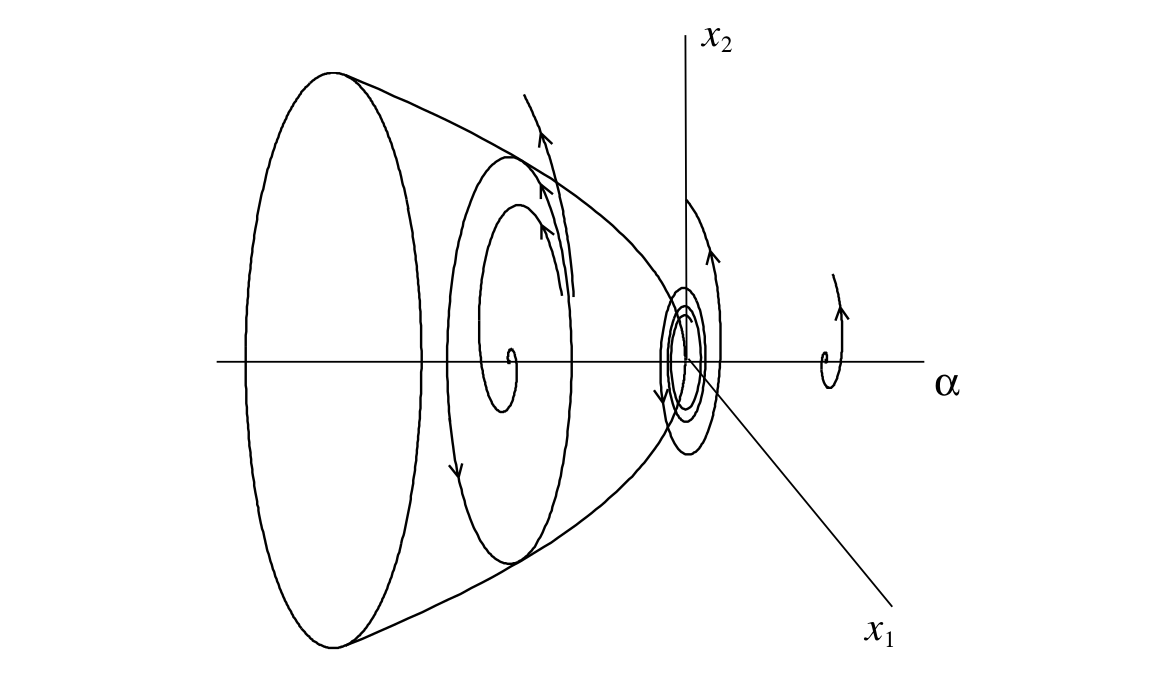
\includegraphics[width=\textwidth]{hopf22.png}
	\caption{Diagrama de bifurcaciones Hopf subcrítica \cite{Kuznet}. }
\label{hopf4}
\end{figure}
	Finalmente incluimos un resultado sobre la forma normal de la bifurcación. Si bien el resultado no nos permite estrictamente conocer la forma normal de esta bifurcación, nos ayuda a dar el primer paso en este sentido. Con el podemos concluir como términos de mayor orden no afectan localmente a nuestra bifurcación, con lo que podremos usar el término de localmente topológicamente equivalentes. Este resultado sirve como catalizador para probar que cualquier sistema, verificándose las hipótesis adecuadas, en el que haya una bifurcación de Hopf, puede ser escrito localmente a través de la forma normal que damos a continuación, concluyendo así el resultado.
	\begin{lemma}
		El sistema 
		\begin{equation}
		\begin{pmatrix}
		x_1' \\
		x_2'
		\end{pmatrix}
		=
		\begin{pmatrix}
		\alpha & -1\\
		1 & \alpha
		\end{pmatrix}
		.
		\begin{pmatrix}
		x_1 \\
		x_2
		\end{pmatrix}
		-(x_1^2+x_2^2)
		\begin{pmatrix}
		x_1 \\
		x_2
		\end{pmatrix}
		+O(x^4).
		\end{equation}
		es localmente topológicamente equivalente cerca del origen a \[ \left \{ \begin{matrix} x'=\alpha x-y-x(y^2+x^2)\\ y'=x+\alpha y-y(y^2+x^2)\end{matrix}\right . .\]
	\end{lemma}
	
	La prueba aunque extensa\footnote{Puede consultarse en el capítulo 3 de \cite{Kuznet}.}, sigue la misma filosofía que la realizada para bifurcación de fold, con ligeras variaciones (como el estudio de la existencia del ciclo límite), dejándonos la forma normal que hemos presentado al principio del apartado.
	
	Esta caracterización responde a un estudio más analítico que cualitativo. Sabemos que la bifurcacion de Hopf se comportarán de una forma similar al comportamiento observado en la forma normal, esto es, los resultados analíticos que apliquemos a la forma normal serán extensibles a nuestro sistema. \\
	
	
	Acabamos, por tanto, exponiendo una caracterización que supondrá un criterio a evaluar cuando necesitemos saber si nos encontramos ante una bifurcación de Hopf. 
	De nuevo la motivación de algunas hipótesis nace en la construcción de la forma normal (genérica) al igual que acontecía en la bifurcación fold.
	
	\begin{theorem}
		Consideremos el sistema:
		\[ \left \{ \begin{matrix} x'=f(x,y,\alpha)\\ y'=g(x,y,\alpha)\end{matrix}\right . .\]
		Donde $alpha$ es nuestro parámetro. Supongamos que tenemos un punto fijo $(x,y)=(x_0,y_0)$ y supongamos que los valores propios del sistema linealizado en un entorno del punto son: $\lambda_{1,2}=a(\alpha)\pm ib(\alpha)$.
		
		Supongamos ahora que para un valor de $\alpha=\alpha_0$ se verifican:
		\begin{enumerate}
			\item $a(\alpha)=0$, $b(\alpha)=\omega\neq0$ donde $sgn(\omega)=sgn[(g_x(x_0,y_0,\alpha_0))]$\\(esta condición nace de la exigencia de tener un par de valores propios imaginarios)
			\item $a_\alpha(\alpha_0)\neq0$\\(Esta condición se obtiene al imponer el cruce del eje imaginario por parte de estos valores)
			\item $\delta=\frac{1}{16}(f_{xxx}+f_{xyy}+g_{xxy}+g_{yyy})+\frac{1}{16\omega}(f_{xy}(f_{xx}+f_{yy})-g_{xy}(g_{xx}+g_{yy})-f_{xx}g_{xx}+f_{yy}g_{yy})$\\(esta condición se obtiene durante la demostración, para justificar que los cambios de variable que se efectúan en ella pueden hacerse)
		\end{enumerate}
		\label{teoremahopf}
	\end{theorem}
	La prueba completa del teorema puede consultarse en \cite{andronof} donde está demostrada por Andronov en su versión en dimensión dos. Si se quiere una generalización se puede consultar\cite{hopfbif} para la traducción de la demostración de Hopf de la extensión de este resultado a dimensión n.
	
\end{enumerate}

\section{Revisitando los osciladores}
Como primera aplicación de este apartado, vamos a recuperar el ejemplo de los osciladores. Comprobamos anteriormente la existencia de órbitas cerradas y ciclos límite. Estudiando este problema sería natural preguntarse si nos encontramos ante una posible bifurcación de Hopf si dejamos libre algún parámetro.
Consideremos de nuevo\ref{vanderpol}:
\begin{equation}
x''-\alpha(1-x^2)x'+x=0.
\end{equation}
Reescribamos el sistema como uno de dos dimensiones de la forma:
\begin{equation}
\left \{ \begin{matrix} x'=y\\ y'=-x+\alpha(1-x^2)y\end{matrix}\right . .
\end{equation} 
Ya sabemos que el único punto de equilibrio es el origen. La matriz Jacobiana del sistema linealizado en un entorno del mismo será:
\begin{equation}
\begin{pmatrix}
0&1 \\
-1 & \alpha
\end{pmatrix}
\label{valooor}
\end{equation}
Por lo que los valores propios de \ref{valooor} serán:\[\lambda_{1,2}=a(\alpha)\pm b(\alpha)=\frac{\alpha\pm i\sqrt{4-\alpha^2}}{2} \]
Comprobamos ahora que se cumplen las hipótesis de \ref{teoremahopf}:
$a(0)=0$, $\omega=b(0)=-1\neq 0$, $a_\alpha(0)=0.5\neq0$.
Por último basta comprobar que $\delta=-1/8\neq 0.$

Estamos pues ante la existencia de una bifurcación de Hopf si variamos el parámetro que aparece en nuestro sistema.Dejamos además un par de gráficas en las que se puede observar este comportamiento: \ref{vander1} y \ref{vander2}

 \begin{figure}[H]
 	\centering
 	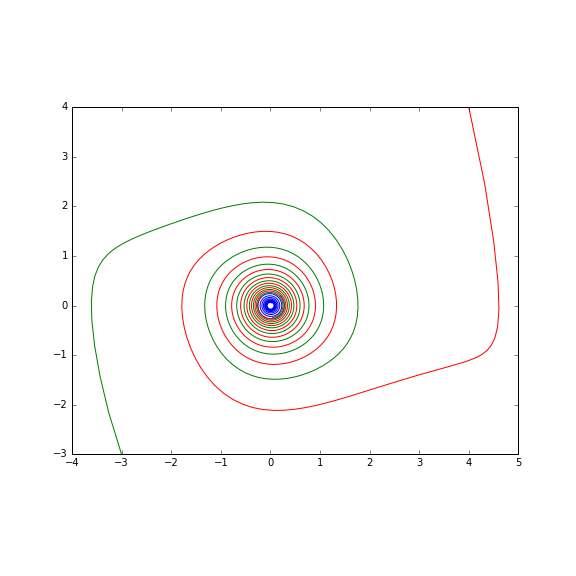
\includegraphics[width=0.5\textwidth]{vanderpol_oscillator2.png}
 	\caption{Comportamiento del oscilador de van der pol con $\alpha=-0.2$}
 	\label{vander1}
 \end{figure}

 \begin{figure}[H]
 	\centering
 	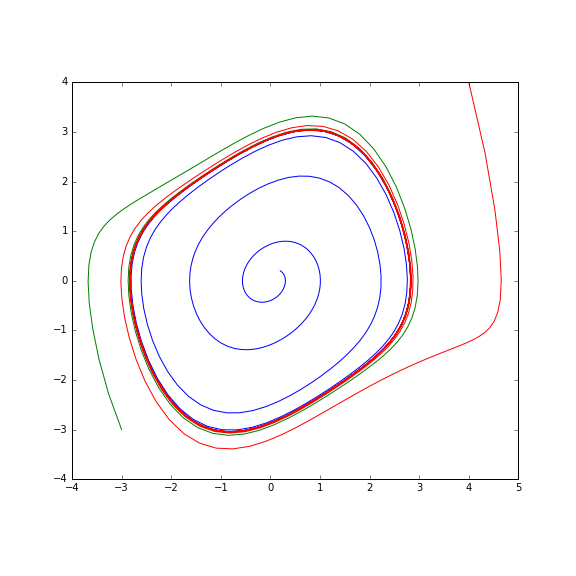
\includegraphics[width=0.5\textwidth]{vanderpol_oscillator.png}
 	\caption{Comportamiento del oscilador de Van der Pol con $\alpha=2.0$ }
 	\label{vander2}
 \end{figure}


\section{Población de gusanos de las píceas}
Uno de los primeros ejemplos de aplicación de estos conceptos se puede encontrar en el estudio de la población de los gusanos de las píceas. El modelo es sencillo, pero lo usamos por que hace aflorar como hasta los esquemas más simples de bifurcación se pueden usar en casos reales.\\
Los gusanos de las píceas son un grupo de insectos con características muy similares dentro del género \textit{Choristoneura}. La mayoría conforman plagas serias para la población de coníferas. Hay cerca de cuarenta especies de Choristoneura, e incluso más subespecies, o formas, con una gran variación entre poblaciones encontradas a través de Estados Unidos y Canadá, y en Eurasia. \\
En particular, como se señala en \cite{Strogatz}, estas plagas ocasionan graves daños al este de Canadá pudiendo acabar con grandes poblaciones de coníferas durante 4 años. 
Es por esto que surgió la necesidad de comprender la dinámica de esta población para predecir cuando encontraríamos explosiones demográficas.
Destacamos que en este modelo no influye la población de árboles, pues su crecimiento es tan lento, que a efectos prácticos su número se considera como una constante \cite{ludw}.

El modelo poblacional responde a la expresión:
\[ y'=Ry\left( 1-\frac{y}{K}\right) -p(y). \]
Donde $y(t)$ representa el número de gusanos de la población, $R$ la tasa de crecimiento y $K$ la capacidad de carga del ecosistema. En ausencia del término $p(y)$ tendríamos un modelo logístico habitual. $P(y)$ es añadido como una tasa que representa la perdida de individuos de la población debido a causas externas (generalmente predadores). Aunque se puede prestar a confusión el porqué esta tasa depende del número de gusanos, tiene una explicación biológica sencilla: cuando el número de gusanos es pequeño los depredadores ignoran las presas (pues cuesta más encontrarse con una de ellas o cazarlas en particular), sin embargo, cuando el número es muy alto, los depredadores aprovechan para alimentarse lo máximo posible. \\
Vamos a profundizar en el caso tratado por Ludwig en 1978 \cite{ludw}, siguiendo el esquema de \cite{Strogatz} a partir de la definición de $p(y)$: 
\[p(y)=\frac{By^2}{A^2+y^2},\]
con las constantes $A$, $ B$ positivas. Quedando nuestro sistema como:
\begin{equation}
y'=Ry\left( 1-\frac{y}{K}\right) -\frac{By^2}{A^2+y^2}.
\label{gusanosss}
\end{equation} 
Para trabajar con (\ref{gusanosss}) vamos a adimensionalizar el sistema. Para ello comenzamos dividiendo por $B$ y haciendo el cambio de variable $y=x/A$,lo que nos deja:
\begin{equation}
\frac{A}{B}\frac{dx}{dt}=\frac{R}{B}x\left( 1-\frac{Ax}{K}\right) -\frac{x^2}{1+x^2}.
\label{gusanossss}
\end{equation} 
Usando esta expresión podemos adimensionalizar el sistema. Para ello llamemos:
\begin{itemize}
	\item $\tau=Bt/A,$
	\item $r=RA/B,$
	\item $k=K/A.$
\end{itemize}
Entonces nuestra ecuación (\ref{gusanossss}) así adimensionalizada queda:
\begin{equation}
\frac{dx}{d\tau}=rx(1-x/k)-\frac{x^2}{1+x^2}.
\label{gusaca}
\end{equation}

Analicemos ahora la estabilidad del sistema:
comencemos por los puntos fijos, que vendrán dados por la ecuación:
\begin{equation}
\begin{split}
0=\frac{dx}{d\tau}=rx(1-x/k)-\frac{x^2}{1+x^2}\Leftrightarrow \\\Leftrightarrow \left \{ \begin{matrix} r(1-\frac{x}{k})=\frac{x}{1+x^2},\\ x=0.\end{matrix}\right .  \label{gusaco}
\end{split}
\end{equation}
Tenemos en primer lugar como punto fijo al $0$, el cual es siempre inestable, algo que podemos comprobar estudiando el signo de la derivada en un entorno del punto cuando $x$ es positivo (no tendría sentido que fuera menor que cero):
\[\text{Sea  }  0<x<k \Rightarrow rx-rx^2/k-\frac{x^2}{x+x^2}>0.\]

Esto se debe a que en un entorno de cero, el término lineal prevalece sobre los cuadráticos. Además, de la igualdad (\ref{gusaco}) podemos ver que para obtener el resto de puntos fijos, basta representar ambas funciones.
Fijado $r$ si variamos $k$ tendremos al menos un punto de intersección, hasta un máximo de 3, en los cuales la función que define nuestro sistema irá alternando estabilidad. Gráficamente podemos observar este comportamiento cualitativo de forma sencilla (Figura \ref{gusanos}).
 \begin{figure}[H]
 	\centering
 	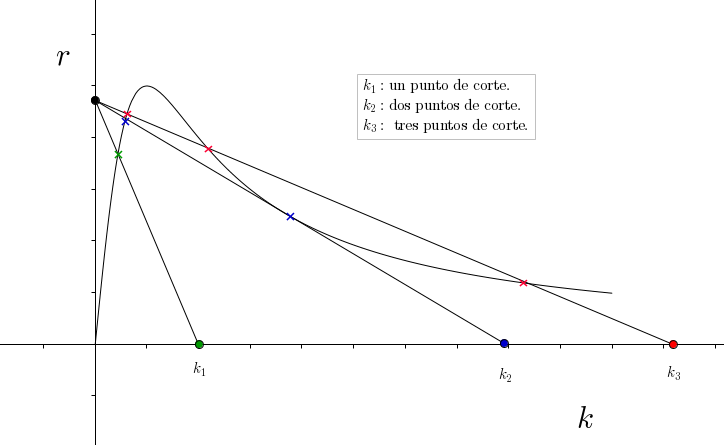
\includegraphics[width=0.8\textwidth]{gusanos.png}
 	\caption{Comportamiento de los puntos fijos según el desplazamiento de k.}
 \label{gusanos}
\end{figure}
Conforme la recta $r,k$ entre en contacto con la curva fijada por x en la segunda parte de la igualdad de (\ref{gusaco}) tendremos la aparición de dos nuevos puntos fijos. Este esquema coincide con el de una bifurcación de fold. 

¿Qué conclusiones podemos obtener?
Debido al cambio de la estabilidad de los puntos fijos, fijado $r$ podemos decir que según aumentemos $k$ tendremos dos regiones de estabilidad determinadas por los dos puntos estables que aparecen. El punto inestable que se origina cuando las nulclinas se intersecan podría entenderse como una cota de cuando el número de insectos va a crecer de forma rápida hasta alcanzar una nueva cantidad de población mayor (Figura \ref{gusanos2}).
 \begin{figure}[h]
 	\centering
 	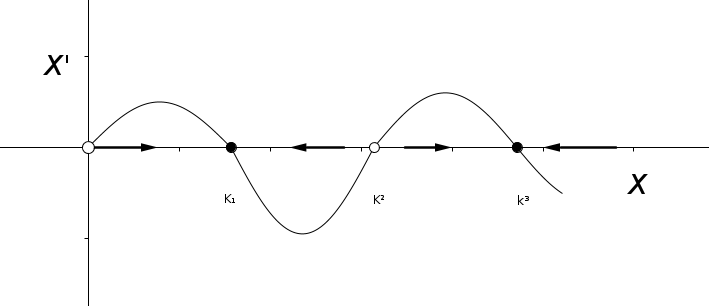
\includegraphics[width=0.5\textwidth]{gusanos2.png}
 	\caption{Estabilidad de los puntos en el caso de mayor k }
 \label{gusanos2}
\end{figure}
Este modelo podría utilizarse para estudiar cuándo las plagas de insectos van a experimentar una explosión demográfica y ajustar el término de sustracción de individuos para que esto no ocurra. 
\section{Glicólisis celular}
Como avanzábamos la bifurcación de Hopf es una bifurcación aplicable a varios campos de la biología, desde poblaciones a dinámica celular.\\En este apartado tratamos un proceso bioquímico fundamental dentro de la biología de la célula. Hablamos de la glicólisis. Mediante este proceso las células vivas obtienen energía metabolizando el azúcar. En células como la levadura, o células musculares, la glicólisis exhibe un comportamiento oscilatorio con las concentraciones de los productos intermedios creciendo y decreciendo en ciclos.

El modelo fue propuesto por Sel'kov en 1986 \cite{sel}. Las variables del mismo representan las concentraciones de ADP (adenosín difosfato) y F6P (fructosa-6-fosfato), además el modelo habitual es completado con dos parámetros que se suponen positivos.\\
El estudio expuesto está basado en los modelos estudiados en \cite{gold} y en \cite{Strogatz}. Desarrollaremos algunas de las operaciones que se realizan para estudiar el modelo, detallando los pasos analíticos a seguir. 

Partimos del sistema adimensionalizado, donde $a$ y $b$ son parámetros positivos \cite{sel}:
\begin{equation}
 \left \{ \begin{matrix} x'=-x+ay+x^2y=f(x,y)\\ y'=b-ay-x^2y=g(x,y).\end{matrix}\right .
\end{equation}
Comencemos el estudio cualitativo del sistema aplicando los conocimientos de la teoría de Poincaré Bendixson, pues observamos en los diagramas de fases la presencia de lo que podría ser comportamiento periódico (Figura \ref{hopf9}).
\begin{figure}[h]
	\centering
	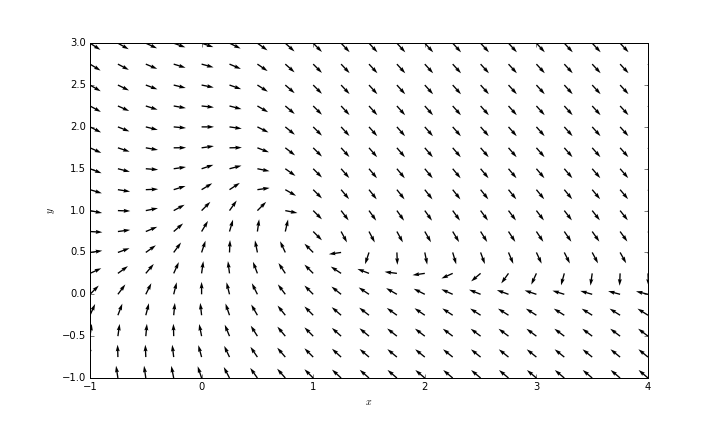
\includegraphics[width=0.7\textwidth]{selkovvv.png}
	\caption{Diagrama de fases de Sel'kov para a=0.5 y b=1 }
	\label{hopf9}
\end{figure}
Dispongamos de las nulclinas del sistema, y además dibujemos los vectores representativos según la zona del espacio en la que nos encontremos. Para ello basta conocer que la dirección del flujo viene determinada por los signos de los vectores. 

\begin{figure}[H]
	\centering
	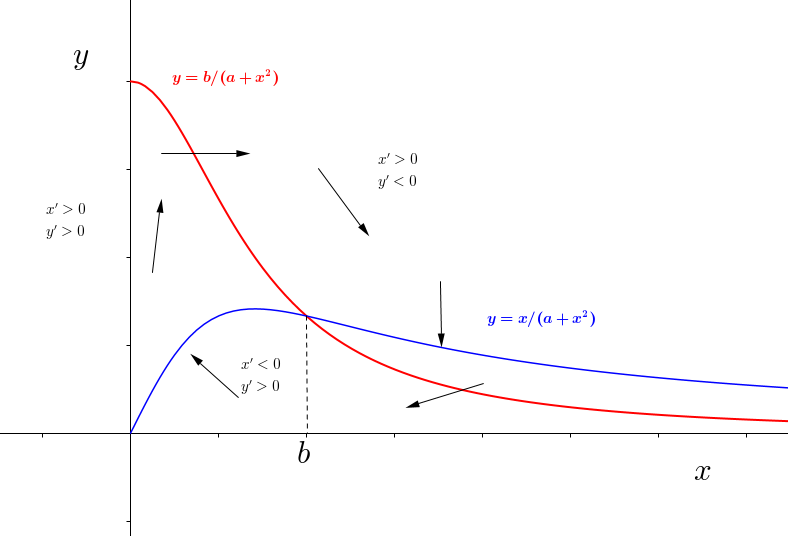
\includegraphics[width=1\textwidth]{hopfnulclinas.png}
	\caption{Nulclinas del modelo de Sel'kov }
\label{hopf7}
\end{figure}

Consideremos una región que atrape las órbitas circulares pues, al respresentar el diagrama de fases, intuimos que esta puede existir. Por ello estudiamos cómo, la región bordeada en la figura \ref{hopf8} es una región dinámicamente invariante, es decir, que cualquier órbita entrante permanecerá en ella.\\ Una posible elección de la frontera podría ser ésta:
\begin{itemize}
	\item $c_1:\left\lbrace x=0;\text{ } 0\leq y\leq b/a\right\rbrace. $
	\item $c_2:\left\lbrace 0\leq x\leq b;\text{ } y= b/a\right\rbrace. $
	\item $c_3:\text{recta entre }(b,b/a)\text{ y la nulclina de x}. $
	\item $c_5:\left\lbrace x=3b;\text{ } 0\leq y\leq \text{punto de corte con la nulclina:}\frac{3b}{a+9b^2}\right\rbrace. $
	\item $c_5:\left\lbrace y=0;\text{ } 0\leq x\leq 3b\right\rbrace. $
	
\end{itemize}
En ella podemos estudiar el comportamiento de los vectores dirección dados por el sistema: 

\begin{figure}[H]
	\centering
	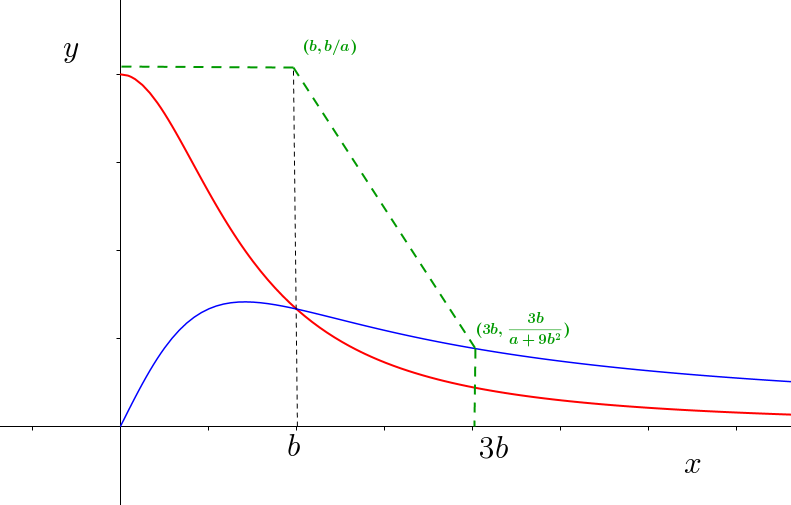
\includegraphics[width=0.7\textwidth]{areahopf.png}
	\caption{Área donde que encierra las órbitas del modelo }
\label{hopf8}
\end{figure}
\begin{itemize}
	\item Para rectas verticales y horizontales, es decir para $ x=0$ $y=0$ no hay problema, el estudio anterior nos confirma el resultado, ya que $f(0,y)=ay\geq0$ y $g(x,0)=b>0$.
	\item La recta que completa nuestra región, es la que va desde el punto $(b,b/a)$ hasta la intersección con la nulclina de $x$. Si tenemos en cuenta que para valores grandes $y'/x'$ se aproxima a  $-1$ esto nos sugiere que para acabar nuestro razonamiento debemos comparar los tamaños de $x'$ e $y'$ para valores suficientemente grandes. Consideramos $x'-(-y')$ y deducimos
	\begin{equation}
	x'-(-y')=-x+ay+x^2y+(b-ay-x^2y)=b-x
	\label{hopf5}
	\end{equation} 
	Por (\ref{hopf5}) tenemos que $-y>x'$ si $x>b$ esto implica que el vector al tener una pendiente más negativa que la recta apuntará hacia el interior de la región que hemos definido.
\end{itemize}
Tenemos pues una región cerrada y acotada, además sabemos que, si existe un valor para $b$ de manera que el punto fijo que aparece en el sistema es de naturaleza inestable, entonces, usando el teorema de Poincaré Bendixson, obtendremos la existencia de ciclos límite.

¿Ahora bien, cómo cambia nuestro sistema una vez fijado $a$?

Para ello deberemos estudiar cómo cambia la estabilidad del punto de corte. Comenzamos calculando el jacobiano:
\begin{itemize}
	\item $\partial f/\partial x=-1+2xy .$
	\item $\partial f/\partial y=a+x^2 .$
	\item $\partial g/\partial x=-2xy. $
	\item $\partial g/\partial y=-(a+x^2). $
\end{itemize}
Por lo que:
\begin{equation}
 J=\left( \begin{array}{ccc}
-1+2xy & a+x^2 \\
-2xy & -(a+x^2) \end{array} \right).
\end{equation}

Además equilibrio del sistema está en :
\[\left\lbrace  \begin{array}{ccc}
-x+ay+x^2y=0,  \\
b-ay-x^2y=0\Rightarrow -b+ay+x^2y=0.
\end{array} \right.
\]
Desde ahi, es claro que para que ambas ecuaciones se anulen, $x=b$ y con esto, sólo queda despejar $y$ de cualquiera de las dos:
\[\begin{pmatrix}
x^*=b \\
y^*=\frac{b}{a+b^2}
\end{pmatrix}.
\]
desde aquí es sencillo estudiar el determinante y la traza de jacobiano en ese punto:
\[\left\lbrace  \begin{array}{ccc}
det(J)=a+b^2>0,  \\
Traza(J)=-\frac{b^4+(2a-1)b^2+(a+a^2)}{a+b^2}.
\end{array} \right.
\]
Si $Traza(J)>0$ no encontraremos con un punto inestable por tanto habrá un ciclo límite. Si $Traza(J)<0$ tendremos uno estable y estaremos ante una espiral.\\
Este es el comportamiento básico de una bifurcación de Hopf pero esto es una mera observación, tenemos que utilizar nuestro criterio. Sin embargo, no debemos olvidar que, tras las cuentas, para comprobar la caracterización ofrecida, deberemos fijar un parámetro (en la formulación de nuestro problema aparecen 2).
 \\
Para ello, con vistas a que el valor del punto fijo interfiera lo menos posible en nuestros cáculos, vamos a desplazarlo al punto $(0,0)$ ,hallando un sistema equivalente. No sólo es una elección que facilita las cuentas, esta decisión también, en el hipotético caso en el que quisiéramos seguir trabajando en nuestro modelo, nos permitiría usar la forma normal para estudiar el comportamiento o las propiedades en las que estemos interesados en un entorno del punto fijo a través de la más sencilla forma normal.
Recogemos aquí los cálculos principales para este propósito:

Si desplazamos el punto hasta $(0,0)$ a través de una sencillo cambio de variables:$\hat{x}=x-b$ y $\hat{y}=y-\frac{b}{a+b^2}$, las derivadas de ambas coinciden y podemos expresar el sistema de la siguiente forma:
\[ \left \{ \begin{matrix} x'=-(x+b)+a(y+\frac{b}{a+b^2})+(x+b)^2(y+\frac{b}{a+b^2}),\\ y'=b-a(y+\frac{b}{a+b^2})-(x+b)^2(y+\frac{b}{a+b^2}). \end{matrix}\right . \]
donde el punto de equilibrio ya está en $(0,0)$.
Calculamos ahora los valores propios de su matriz jacobiana:
\[\begin{pmatrix}
-1+\frac{2b^2}{a+b^2} & a+b^2 \\\frac{-2b^2}{a+b^2} & -a-b^2
\end{pmatrix}.
\]
 de donde los valores propios obtenidos serán:

\[ \lambda_{1,2}(a,b)=\frac{a+a^2-b^2+2ab+b^4\pm i \sqrt{4(a+b^2)^3-(a(1+a)+(-1+2a)b^2+b^4)^2}}{-2(a+b^2)}.\]
Al final del procedimiento vamos a fijar el parámetro $a$, por lo que a la hora de comprobar si se satisfacen las condiciones será el valor de $b$ el utilizado (por lo que durante los cálculos dependerá de $a$).

Para que la parte real se anule necesitamos:
\[ b_{1,2}=\sqrt{(1\pm\sqrt{1-8a}-2a)/2} .\]
La segunda condición (que recordemos exige derivar respecto de un parámetro y nosotros hemos elegido $b$) impone:

Si $b=b_1(a)$:
\[ \frac{d\Re(\lambda_1)}{db}=\frac{\sqrt{2-16a}\sqrt{(1-\sqrt{1-8a}-2a)}}{(1-\sqrt{1-8a})}. \]
Si $b=b_2(a)$:
\[\frac{d\Re(\lambda_2)}{db}=\frac{\sqrt{2-16a}\sqrt{(1+\sqrt{1-8a}-2a)}}{(-1-\sqrt{1-8a})}.\]

Por último el valor de la expresión de la tercera condición para $b_1$ y $b_2$ vendrá determinado por:
\[-\frac{1}{8}-\frac{(a+b^2)(\frac{b}{a+b^2}+y)^3}{2\sqrt{4(a+b^2)^3-(a(1+a)+(-1+2a)b^2+b^4)^2}}\]

Por tanto, fijado $a$, podremos conocer el valor de $b$ sea nuestra elección cualquiera de las dos posibles y determinar si se cumplen las condiciones de la caracterización. En los $b$ en los que esto ocurra podremos afirmar tener una bifurcación de hopf y, dado que hemos desplazado nuestro punto fijo al $(0,0)$ sabremos que en un entorno se comportará como la forma normal (las cuentas así como un ejemplo de valores posibles se pueden observar en \cite{student}).





\chapter{Análisis Numérico}

\label{ch:numerico}

\section{Principios generales para el tratamiento numérico de bifurcaciones}
Es de suponer por todo lector, tras los ejemplos vistos anteriormente, que estudiar analíticamente las bifurcaciones de sistemas dinámicos con origen biológico se vuelve, en la mayoría de los casos una tarea bastante ardua. Por eso mismo surge, inevitablemente, el estudio numérico de los comportamientos no sólo anteriormente descritos sino, de todos los que de alguna manera se relacionan con la descripción cualitativa de sistemas dinámicos.\\
En particular vamos a introducir en este apartado los conceptos básicos y métodos más utilizados para el estudio cualitativo de algunas de las bifurcaciones del capítulo anterior.\\
En esta exposición vamos a tratar el estudio de sistemas con un parámetro libre, los métodos serán generalizables a distintas disyuntivas. Procedemos de esta manera debido a que exponerlos todos sería a priori una tarea hercúlea y desde un primer momento inabarcable, puesto que para cualquier cambio que se aleje de este marco, supondrá un cambio notable en los métodos (véase \cite{Lectures} y \cite{prac}). Además no hemos de olvidar que nuestro sistema no tiene porqué ser uniparmetrico, lo único que exigimos para este estudio es que el resto de los parámetros estén fijados.
\subsection{Presentación del problema}
Partimos de un sistema dinámico uniparamétrico (o multiparámetro si mantenemos todos los parámetros fijos excepto uno) el cual queremos estudiar cualitativamente. A priori dada la naturaleza de nuestro problema, solemos contar con un rango de valores paramétricos sobre los que realizamos el estudio.\\
Supongamos que el rango de parámetros de interés es $\alpha_a \leq \alpha \leq \alpha_b $. A través de nuestro algoritmo de resolución calcularemos la primera de ella $\alpha_0=\alpha_a$. Como es de suponer este paso en general no será ni inmediato ni sencillo.  
Suponemos por tanto que la solución se puede calcular para  $\alpha_0=\alpha_a$.
Después de haber tenido éxito con  $\alpha_0=\alpha_a$, la siguiente pregunta es cómo elegir  $\alpha_1$.\\Un enfoque útil podemos encontrarlo en los fundamentos de las asignatura de análisis numérico de EDP's. Intuitivamente podríamos pensar que si utilizamos una partición equidistante con una cantidad de nodos cualesquiera (previamente escogidos), obtendríamos de ella una buena manera de elegir el valor de los parámetros subsiguientes de nuestro estudio.
Sin embargo es habitual que usando esta estrategia nos encontremos tres aspectos problemáticos a solventar:
\begin{itemize}
	\item  Se puede pasar por alto una bifurcación.
	\item  Un punto de inflexión o giro ocurre: una bifurcación fold (Figura \ref{diagfold}), y nuestro algoritmo de resolución no funciona adecuadamente.
	\item \textit Aumento del coste computacional: tratar el problema con un espacio muy pequeño puede ocasionar costes elevados.
\end{itemize}
A modo de esquema-resumen, aunque veremos los pasos con más detalle en los siguientes apartados, para paliar las disposiciones más delicadas debemos contar con estas herramientas: \\
Lo primero que necesitamos es \textit{un método de continuación}. Este método genera una cadena de soluciones, además, los candidatos razonables para el incremento de nuestro parámetro son calculados de forma adaptativa. Además el método también puede complementarse con un chequeador de la estabilidad de la rama que estamos estudiando.\\
Por otra parte necesitaremos una forma de detectar y clasificar las bifurcaciones si este método las encuentra.\\
Por último, en muchas ocasiones se puede observar el añadido de un algoritmo que nos permita saltar entre las ramas del diagrama. Es necesario, por tanto, que nuestro método se capaz de calcular distintas ramas de soluciones, pues esto es lo que nos dará una visión acertada global, sin embargo no incluimos aquí la teoría asociada para no extender en demasía el trabajo,  lo que nos permite dar una idea general del método que puede ampliarse con la bibliografía.

\subsection{Cálculo de soluciones iniciales}
Antes de comenzar con los métodos propiamente dichos, me permito profundizar ligeramente en este apartado. En el mismo inicio de nuestro estudio nos encontramos ante este problema:
\begin{equation}
x'=f(x,\alpha_0), x\in\mathbb{R}^n, \alpha\in\mathbb{R},
\end{equation}
de donde queremos obtener las soluciones de la ecuación:
\begin{equation}
0=f(x,\alpha_0), x\in\mathbb{R}^n, \alpha\in\mathbb{R}.
\end{equation}
Es decir, los puntos fijos. A la solución de este problema es a la que le aplicaremos la continuación para obtener el resto de valores. Ahora bien, para ello debemos comenzar con algún valor de nuestro parámetro y, sea cual sea, puede que esta tarea se nos presente muy difícil. Por ello, normalmente, se siguen un par de estrategias éstandar (\cite{Lectures}, \cite{prac}, \cite{siam1} y \cite{graduate}):
\begin{itemize}
	\item Discutir las soluciones de problemas derivados del nuestro de forma que estas sean un caso particular simplificado que nos ayude.
	\item Tomar el rango de valores del parámetro de manera que el primero de ellos simplifique nuestro sistema (en general suele usarse $\alpha_0 =0$).
\end{itemize} 

He de resaltar que en este paso se utiliza un concepto adaptado que nos introdujeron en la asignatura de Topología II: la homotopía. \\
El concepto de homotopía en este contexto surge de la necesidad de resolver una ecuación que a priori se nos presenta difícil. En general el problema no es exclusivo del estudio de bifurcaciones, por lo que, por comodidad notaremos $(x,\alpha)=y$.\\
Supongamos pues que tenemos una expresión de la forma $g(y)=0$ que queremos resolver.
Supongamos que tenemos $f(y)=0$ que es una función sencilla, obtenida de simplificar nuestra $g(y)$ inicial, y que es fácil de resolver. El concepto de homotopía consiste en construir una sucesión de n ecuaciones, que resueltas una a una en orden consecutivo, nos permita llegar a solucionar nuestra ecuación inicial:
\[ f_{0}(y)=f(y)=0\rightarrow f_{1}(y)=0\rightarrow\dots \rightarrow f_{n-1}(y)=0 \rightarrow f_{n}(y)=g(y)=0. \]
La diferencia entre dos términos debe ser lo suficientemente pequeña para que así también lo sea las soluciones asociadas a cada uno.\\
La caracterización anterior no es mas que una versión discreta del proceso de homotopía y, al uso, seguimos teniendo el problema de definir adecuadamente las funciones intermedias. Este escollo lo podemos solventar traduciendo nuestro problema a una formulación continua y, tras ello aplicar métodos de continuación estándar. 
Usemos $0 \leq\lambda\leq 1$ con $\lambda \in \mathbb{R}$ y construyamos una funcion
\begin{equation}
f^{hom}(y,\lambda)=0,0 \leq\lambda\leq 1. 
\label{homotopi}
\end{equation} 
tal que 
\[ f^{hom}(y,0)=f(y) \text{ y } f^{hom}(y,1)=g(y). \]
El problema ahora puede ser la forma de escoger (\ref{homotopi}). Esto es ya sin embargo terreno del estudio de cada problema. Planteamos aquí alguna elección estándar como puede ser:
\begin{equation}
f^{hom}(y,\lambda):=\lambda g(y)+(1-\lambda)f(y).
\label{homotopi2}
\end{equation} 
De hecho soluciones incluso más sencillas (y mucho más complejas) se han encontrado útiles\cite{allgower}.

Es también reseñable como este problema está intrínsecamente relacionado con parte de  nuestro problema inicial, uniendo conceptos que se nos muestran en topología con el cálculo de las ramas de un diagrama de bifurcaciones (presentados en el tema anterior). Este hecho nos muestra como la interconexión de ideas puede ser altamente fructuosa en métodos numéricos.
\subsection{Método de continuación}
Describiremos en esta sección la caracterización método de continuación, así como varios métodos numéricos aplicables en cada caso. Lo haremos desde una perspectiva adaptad a las bifurcaciónes aunque, como veremos, es un método que se puede utilizar para multitud de problemas.
\subsubsection{Planteamiento}
Nuestra intención es estudiar los puntos de equilibrio de un sistema dada la variación de un parámetro. Como sabemos estos puntos vienen determinados (su existencia, no su estabilidad) por la anulación de la función que determina el sistema.\\
Consideremos, pues, un sistema continuo:
\begin{equation}
x'=f(x,\alpha),\text{ } x\in\mathbb{R}^n, \text{ }\alpha\in\mathbb{R}.
\label{formulacionbasica}
\end{equation}
Donde f es una función suficientemente derivable. Los puntos de equilibrio de (\ref{formulacionbasica}) satisfacen
\begin{equation}
f(x, \alpha) = 0.
\label{cero}
\end{equation}
Es decir, un sistema de n ecuaciones escalares en $\mathbb{R}^{n+1}$. Generalmente (\ref{cero}) define una curva (o en cualquier caso una variedad 1-dimensional) $M$, en $\mathbb{R}^{n+1}$. El cálculo de esta
variedad proporciona la dependencia de un equilibrio de (\ref{formulacionbasica}) con respecto al parámetro  de nuestra formulación.\\
El problema de calcular la curva M es el prototipo del caso de estudio de los problemas de continuación:
\begin{equation}
f(x,\alpha)=0,\text{ } f:\mathbb{R}^{n+1}\rightarrow\mathbb{R}^n.
\label{cumplir}
\end{equation}
Por el Teorema de la Función Implícita, el sistema (\ref{cumplir}) define localmente un
curva $M$ que pasa por cada punto $(x_0,\alpha_0)$ que satisface (\ref{cumplir}), siempre que el $rango(J)
= n$, donde $n$ es el número de equaciones que definen el sistema, y $J$, es la matriz jacobiana de (\ref{cumplir}) en $(x_0,\alpha_0)$.\\
La solución numérica del problema de continuación (\ref{cumplir}) nos aportará una sucesión de puntos que nos permitirán aproximar $M$ en mayor o menor exactitud. Habitualmente, utilizando los métodos de resolución convencionales comenzaremos por un $(x_0,\alpha_0)$ lo mas aproximado a $M$ posible. \\Con este fin, se siguen estrategias estándar basadas en hallar un punto de equilibrio a partir del cual comenzar. Fijada habitualmente una homotopía y usando algoritmos de resolución, como el método de Newton, para aproximar este punto inicial. Veremos en el siguiente apartado un estudio más concreto de estos métodos, centrándonos en aquello que usa el software que utilizamos. 

La mayoría de los algoritmos de continuación utilizados en el análisis de bifurcaciones se basan en la implementación de \textbf{Métodos de predicción-corrección} como puede verse en casi todos los libros de esta temática, por citar varios: \cite{Lectures}, \cite{siam1}, \cite{auto}. Estos métodos se componen de tres subetapas que pasamos a describir con mas detalle:
\begin{enumerate}
	\item predicción del siguiente punto,
    \item corrección del punto calculado,
    \item control de tamaño de paso o discretización.
\end{enumerate}

\subsubsection{Predictores}
Comenzamos con la discusión de los predictores. Básicamente los predictores son un mecanismo que nos permiten dar una estimación inicial o \textquotedblleft poco refinada\textquotedblright de lo que será el siguiente par $(x,\alpha_n)$ a estudiar en nuestro problema \ref{cumplir} . Los predictores se pueden dividir en dos clases \cite{prac}:
\begin{itemize}
	\item  Métodos basados en ecuaciones diferencial, es decir que se basan en $f (x, \alpha)$ y sus derivadas.
	\item Métodos basado en extrapolación polinomial, que utiliza sólo soluciones $(x, \alpha)$ de la ecuación (\ref{cumplir}).
\end{itemize}
 En general, para este apartado se suelen utilizar métodos muy estandarizados dejando un poco el refinamiento de estos a la parte de corrección. En nuestro caso vamos a comentar dos de ellos con el fin de mostrar la filosofía de los mismos:
\begin{itemize}
	\item Predictor tangente\\
Tomando la derivada de ambos lados de la ecuación (\ref{cero}), se obtiene
\begin{equation}
0 = df = f_x dx + f_\alpha d\alpha, \label{44}
\end{equation} 

y por lo tanto
\[\frac{dx}{d\alpha}= -(f_x)^{-1}f_\alpha. \]

Integrando este sistema a partir de los valores iniciales $(y_1, \alpha_1)$, se obtiene
la curva $M$ en la que $(y_1, \alpha_1)$ se encuentra. Este procedimiento, propuesto por \cite{georg}, falla en puntos de inflexión debido a la singularidad que se forma en estos puntos por $f_y$. Esto es solventable a través de varias estrategias siendo las más común cambiar el parámetro que estamos evaluando o considerar $x$ y $\alpha$ como funciones dependientes del parámetro arco \cite{prac}.

Esta idea sirve de germen para uno de los predictores más usados. Hablamos del \textbf{Predictor tangente}. Introducimos notación: Sea $z_i = i-esima$ componente de $z$ y, $ z_i = dx_i (1 \leq i \leq n), z_{n+1}= d\alpha$.

Con esta notación podemos transformar (\ref{44}) en la ecuación
\begin{equation}
(f_x | f_\alpha)\cdot z = 0.
\end{equation}
Entiéndase $(f_x | f_\alpha)$ como una matriz de vectores columna adjuntados y, $z$, como un vector tangente.\\
¿Qué podemos decir sobre z? En primer lugar, la recta que contiene al vector es única (aquí estamos asumiendo que $(f_x | f_\alpha)$ tiene rango máximo). Por otra parte el módulo y la orientación del vector z nos son desconocidas. Para obtener una solución única debemos imponer condiciones de normalidad: basta por ejemplo $e. z = 1$ con $e$ algún vector unitario (n+1)-dimensional.\\

En general la formulación de estos métodos puede escribirse como:
\begin{equation}
(x^{j + 1}, \alpha_{j + 1}): = (x^j, \alpha_j) + \sigma_j z_j. \label{normalizao}
\end{equation} 
 Donde $\sigma_j$ es una longitud de paso apropiada. El concepto de apropiedad puede parecernos pernicioso, pero comprobaremos que es habitual que la longitud cambie para adaptarse a nuestro problema (ver \ref{longitud} - Longitud de paso).

Este predictor tangente puede considerarse un paso del método de Euler para resolver una ecuación diferencial que describe la curva $M$, o, lo que es lo mismo, una aproximación de Taylor de orden 1. Por lo tanto, el error de discretización conocido por la asignatura de métodos numéricos II se puede aplicar aquí, obteniendo un error de orden 1.

\item Extrapolación polinomial:\\
Las ideas de extrapolación polinomial también pueden usarse para el paso de predicción. En este caso el método  se basa en la creación de  un polinomio en $\alpha$ de grado $n$ que pasa por los puntos:
\[ (x_j, \alpha_j), (x_{j-1}, \alpha_{j-1}),. . . , (x_{j-n}, \alpha_{j-n}). \]
Si suponemos que este polinomio proporciona una aproximación a $M$ en la región en la que calculamos, un predictor será evaluar la función en  la continuación $\alpha \equiv \alpha_{j + 1}$. 
Usando un polinomio de primer orden ,obtenemos el predictor secante que es la alternativa al predictor tangente (\ref{normalizao}), añadimos también un normalización:
\begin{equation}
Prediccion: ( x_{j + 1}, \alpha_{j + 1}): = (x_j, \alpha_j) + \sigma_j \frac{(x_j - x_{j-1} , \alpha_j - \alpha_{j-1})}{|(x_j - x_{j-1} , \alpha_j - \alpha_{j-1})|}.
\label{secant}
\end{equation}
 Con $\sigma_j$ como longitud de paso y en este caso $z=\frac{(x_j - x_{j-1} , \alpha_j - \alpha_{j-1})}{|(x_j - x_{j-1} , \alpha_j - \alpha_{j-1})|}. $
\end{itemize}
 Es frecuente, como se expone en (\cite{prac}),que  los predictores de orden inferior (tangente, secante) son a largo plazo menos costosos y por lo tanto preferidos. El error de discretización del predictor secante de (\ref{secant}) es del mismo orden que el predictor tangente.\\
 Añadimos además un pequeño esquema para visualizar la diferencia entre ambas en la figura \ref{tangent}.
  \begin{figure}[h]
  	\centering
  	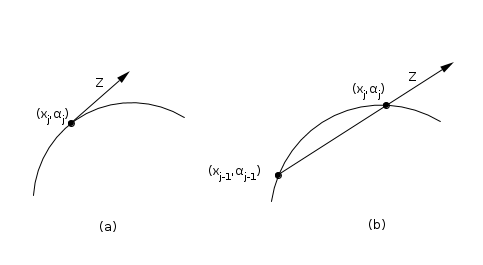
\includegraphics[width=0.7\textwidth]{predic.png}
  	\caption{Representación del predictor tangente (a) y secante (b)}
  	\label{tangent}
  \end{figure}
 En general, la filosofía de estas aproximaciones (debido en parte a que son las más básicas que se usan) ya apareció en la asignatura de métodos numéricos II.
\subsubsection{Correctores}
 Una vez hemos predicho $( x_{j + 1}, \alpha_{j + 1})$, que suponemos suficientemente cercano a nuestra curva, vamos a aplicar un paso para refinar esta predicción y dar con nuestro candidato. Es lo que conocemos como \textbf{Corrección}. Mediante este paso vamos a intentar localizar el que será el siguiente punto de nuestra recta de forma definitiva con una determinada precisión (que impondremos nosotros).
 
 Para este paso normalmente se utilizan técnicas de resolución basadas en el método de Newton, para ello necesitamos el mismo número de ecuaciones que de incógnitas si queremos poder aplicarlo.\\
 La forma habitual de estar seguros de tener el número correcto de ecuaciones es añadir el parámetro mediante el cual vamos a parametrizar nuestra curva $M$. Pues si establecemos nuestra parametrización mediante una ecuación escalar adicional: $g^j(x,\alpha)$ podemos extender el sistema y aplicar así el método de Newton en:
 \[\left\lbrace  \begin{array}{ccc}
 f(x,\alpha)=0,  \\
 g^j(x,\alpha)=0.
 \end{array} \right.
 \]
  De hecho en muchos casos este concepto entiendo puede entenderse geométricamente como intersecar la recta $M$ con una hipersuperficie cercana a nuestro punto. Para facilitar la notación, de nuevo, denotemos $(x,\alpha)=y$, $(x_j,\alpha_j)=y_j$ para el punto definitivo y $(x_j,\alpha_j)=\tilde{y}_j$ para el predicho.
 \begin{itemize}
 	\item \textbf{Continuación por pseudo-longitud de arco }
 	
 	En este caso vamos a seleccionar el hiperplano que pasa por el punto $\tilde{y}_{j+1}$ que es ortogonal al vector $z$, es decir, nuestra funcion corrección estará definida como:
 	\begin{equation}
	g^j(x,\alpha) =\langle y-\tilde{y}_{j+1},z\rangle =\langle y-y_{j},z\rangle-\sigma_j.
	\label{pseudoarco}
 	\end{equation}
 	Si la curva es regular y el tamaño del paso $\sigma_j$ es suficientemente pequeño, se puede probar \cite{Keller}, que las iteraciones de Newton para el sistema formado por el paso de corrección y (\ref{cumplir})  convergerán a un punto $y_{j+1}$ sobre la curva $M$ desde el punto predicho $\tilde{y}_{j+1}$.
 	
 	\item \textbf{Continuación Moore-Penrose} 
 	Mencionamos este caso porque además de ser muy utilizado \cite{allgower} introduce un nuevo cambio al estándar de los pasos de corrección. En cada iteración del método de Newton, nuestra función correctora variará. El plano o curva donde estamos iterando puede hacerse ortogonal a un vector normalizado que satisfaga que el producto escalar de este vector por el jacobiano en el punto anterior sea 0 ($J(Y_{j-i}).V^k=0$) por lo que obtendríamos la siguiente función: 
 		\begin{equation}
 		g^j_k(y) =\langle y-Y_{j + 1},V^k\rangle .
 		\label{moore}
 		\end{equation}
 \end{itemize}

\subsubsection{Longitud de paso}
\label{longitud}
Como se puede esperar hay muchos algoritmos sofisticados para controlar el tamaño del paso $\sigma_j$ \cite{Keller} sin embargo, sorprendentemente uno de los más utilizados, por su fácil implementación y moderada fiabilidad es disminuir el tamaño del paso y repetir las correcciones si no se produce convergencia después de un número prescrito de iteraciones. Si la situación cambia y la convergencia requiere pocas iteraciones aumentamos el tamaño del paso $\sigma_{j + 1}$ con respecto a $\sigma_j$ si la convergencia y, mantenemos el paso actual $\sigma_{j + 1} = \sigma_j$ si la convergencia ocurre después de un número prefijado como aceptable de iteraciones. Esta es la idea básica de los métodos de paso adaptativos, los cuales, como avanzábamos, poseen una literatura enorme.

\subsection{Localización de Bifurcaciones}
Inevitablemente, durante el proceso de construcción de nuestro diagrama de bifurcaciones pasaremos por algunas de ellas. Por tanto para complementar la construcción numérica debemos ser capaces de construir métodos para este fin. 
Supongamos que tenemos una sucesión de soluciones que ha sido aproximada:
\begin{equation}
(x_1, \alpha_1), (x_2, \alpha_2),...
\end{equation}
Supongamos además, que entre dos de ellas: $ (x_{j+1}, \alpha_{j+1})$ y $(x_j, \alpha_j)$ se halla un punto de bifurcación. Nuestro problema será reconocer,  partir de las soluciones, si una bifurcación está cerca.

De nuevo, nos encontramos ante una gran variedad de posibilidades \cite{Kuznet,prac,Lectures} solo copadas por la imaginación de los matemáticos actuales, sin embargo, vamos a introducir aquí una de las más utilizadas que, de hecho, también es la más sencilla.\\
La conclusión sobre si estamos ante un punto de bifurcación vendrá determinada por una función de prueba o función test: $T(x, \alpha)$, que se evalúa durante el proceso de construcción de la curva. Una bifurcación vendrá indicada cuando nuestra función test se anule, es decir:
\begin{defi}
	Una función test para bifurcaciones es una función que satisface la propiedad
	\[T(x_i,\alpha_i)=0\]
	si en $(x_i,\alpha_i)$ hay un punto fijo que experimenta una bifurcación o, convencionalmente, si en $(x_i,\alpha_i)$ hay una bifurcación. Además, es continua en un intervalo suficientemente grande que incluye a $\alpha_i$
	\label{funtest}
\end{defi} 
Los criterios test habitualmente se nos presentan \cite{Lectures,prac}, como una caracterización necesaria, es decir, si nuestra función se anula entonces estaremos ante una bifurcación. Además es usual detectar un punto de bifurcación si nos encontrarnos con un cambio de signo en la función test, puesto que es evidente que tengamos el tamaño de paso que tengamos, sea fijo o variable, no es habitual encontrar el punto exacto.\\ Teniendo esto en cuenta es habitual que nuestro criterio pase a ser:
\begin{equation}
T(x_{j+1}, \alpha_{j+1}) T (x_j, \alpha_j) <0.
\label{crite}
\end{equation}
Puede consultarse en la sección de ejemplos una muestra de aplicación en un caso real \ref{line:sp}.

Una elección temprana, pero igualmente válida puede ser establecer nuestra función test como el máximo de todas las partes reales de nuestros valores propios asociados al jacobiano de nuestro sistema:
\begin{equation}
T:=max\{\Re(\lambda_1),...,\Re(\lambda_n)\}
\label{ftest1}
\end{equation}
Esta función es particularmente significativa puesto que $T<0$ garantizaría estabilidad local. Además si $f(x,\alpha)$ es derivable la función test \ref{funtest} es continua aunque no necesariamente derivable.

Sin embargo, podemos plantear perfectamente el problema de que esta función test no señalará comportamientos si la bifurcación se encuentra en la intersección de dos ramas inestables (ambas partes reales serán negativas). Una buena forma de sobrevenir este problema es modificar nuestra función de partida \cite{funci} y escribirla como:
\begin{equation}
T:=\Re(\lambda_k) \text{ con } |\lambda_k|=min\{|\lambda_1|,...,|\lambda_n|\}
\end{equation}

La función test más utilizada puede obtenerse recurriendo a la propia caracterización de las bifurcaciones fold (o en general de todos puntos donde encontramos una bifurcación), en tanto que en ellas el Jacobiano es singular.:
\begin{equation}
det(f_y(y_0,\alpha_0))=0.
\end{equation}
Teniendo esto en cuenta podemos usar como función test:
\begin{equation}
T(y,\alpha)=det(f_y(y_0,\alpha_0)).
\label{2test}
\end{equation}
Una ventaja que observo de esta función es la conveniencia numérica, pues al realizar la continuación debemos calcular el jacobiano (si seguimos el procedimiento del apartado anterior) y, por tanto, a poco que se piense en la programación del método de Newton, se verá que podemos ahorrarnos el calculo de la función test, aprovechando los residuos del método de Newton.
Típicamente, como vimos en la asignatura de Métodos Numéricos I, el jacobiano puede atacarse a través de la descomposición LU. Así, nuestro jacobiano quedará de la forma:
\begin{equation}
Pf_y=LU
\end{equation}
Donde P es una matriz de permutación. Realizando el determinante en ambas partes:
\[ \pm1  det f_y=1.det U\]
de donde
\[ T= \pm det U \]
Debido a que el determinante de una matriz triangular es igual al producto de los elementos de la diagonal principal, $det U$ y por lo tanto $|T|$ son fácilmente calculables. Aún así debemos prestar atención a tomar el signo correcto de $T$, que depende del de la permutación.

 Como con todas las pruebas de bifurcación, la exactitud de $T$ depende de la precisión con que la que el jacobiano sea evaluado . Además me gustaría destacar que hay dos inconvenientes conocidos para el método \ref{2test}:
 \begin{itemize}
 	\item Evaluar la expresion (\ref{2test}) resulta costosa para sistemas grandes
 	\item El orden de magnitud de (\ref{2test}) puede ser mur grande, esto es: puede resultarnos difícil comparar valores de $T$, por ello, a su vez, ser críticos con tamaños de paso u otros parámetros.
 \end{itemize} 
 
Habitualmente nos encontraremos como a parte de criterios específicos para cada bifurcación, este criterio se incorpora. De nuevo el fragmento de código \ref{line:sp} es un buen ejemplo de ello. Nótese que en ese caso BP hace referencia a Bifurcation Point (criterio para punto de bifurcación).

 Siguiendo la filosofía de la función anterior, es decir, centrarnos en el comportamiento de los valores propios según exista una bifurcación u otra, añado una función test que nos puede ser útil para detectar bifurcaciones de Hopf \cite{Kuznet,prac}:
 \begin{equation}
 T(y,\alpha)_\text{Hopf}=\Pi_{1\leq k<j\leq n}(\lambda_j+\lambda_k)
 \label{3test}
 \end{equation}
 Donde $\lambda$ representa valores propios. Si recordamos la caracterización inicial en el \textit{Capítulo 2} de la bifurcación de Hopf, vemos que en el punto de la bifurcación tendremos dos valores propios imaginarios y complementarios.\\
 Es de destacar que la función test también se anula para valores reales opuestos, por lo que los programas suelen implementar formas de desechar estos datos o directamente utilizar otros métodos mas complejos como las matrices bialternadas en \cite{Kuznet}.
 \subsection{Método de Newton-Chord}
 Para acabar este apartado vamos a presentar la modificación del método de Newton que se presenta en el software que más adelante presentamos.\\
 Como hemos hecho notar a través de la sección anterior es habitual proceder en los métodos de continuación mediante iteraciones tipo Newton. En particular en nuestro caso vamos a destacar el método Newton-Chord.
 Habitualmente no es común poder tener la expresión explicita del Jacobiano, de hecho computacionalmente es una de las partes más costosas (nos referimos aquí al cálculo del jacobiano y de su valor). Por ello multitud de métodos \cite{siam1} se centran en utilizar la filosofía de las iteraciones del método de newton pero evitando el cálculo del Jacobiano. En este marco tenemos la definición del método de Newton-Chord.
 
\begin{defi}[Método de Newton-Chord]
	Sea $x_0$ un número suficientemente cerca de la solución de una ecuación de la forma $F(x)=0$, definimos las \textit{iteraciones del método de Newton-Chord} como:
	\[ x_{n+1}=x_n-F'(x_0)^{-1}F(x_n). \] 
\end{defi}
 
 Es decir, afrontamos el problema del gasto computacional utilizando en todas nuestras iteraciones el Jacobiano (o en $\mathbb{R}^1$, la derivada) calculado en el mismo punto.
 
 Complementario a este apartado, dejamos un resultado, que nos muestra el \textit{precio a pagar} por utilizar este método, es decir, la disminución del orden de convergencia. 
 Dadas las siguientes suposiciones:
 \begin{itemize}
 	\item $F(x)=0$ tiene solución.
 	\item $F':\Omega \rightarrow \mathbb{R}^{N\times N}$ es lipschitciana.
 	\item $F'(x)$ es no-singular.
 \end{itemize}
 \begin{theorem}
 	Existe $\delta>0$ de manera que si $x_0$ pertenece a una bola de centro la solución y radio $\delta$ entonces las iteraciones de Newton-Chord convergen a la solución. Sin embargo:
 	\[ |x_{n+1}-x_{sol}|<k|x_n-x_{sol}| \]
 	para algún $0<k<1$.
 \end{theorem}
 La prueba sigue una filosofía similar al propio método de Newton, puede consultarse en \cite{siam1} para su desarrollo completo. En líneas generales la idea es construir un sistema dinámico discreto con la formulación de las iteraciones. Si este sistema define una aplicación contractiva el Teorema de Punto Fijo de Banach asegura la convergencia. 
 Además, como se puede ver, la convergencia es linear (Newton sin embargo posee convergencia cuadrática, es decir: $|x_{n+1}-x_{sol}|<k|x_n-x_{sol}|^2$ ).
 
 Resaltamos por tanto que métodos que en un principio pueden parecer mejores, se demuestran en la práctica sobrepasados por otros, debido a que, aunque la convergencia tenga menor orden, los cálculos implicados tienen un coste computacional menor.  

 \section{Software utilizado}
 En esta sección recogemos el conjunto del software que recoge las ideas analíticas y numéricas de los capítulos 2 y 3 y, nos sirve para realizar el análisis cualitativo de todos los modelos vistos en el trabajo.\\ Se han utilizado dos herramientas principales para el estudio y una opcional para la visualización dinámica.
 
  \subsection{Python: Diagramas de Fases}
  Pyhton y sus librerías especializadas \cite{Python} se han convertido en toda una referencia para trabajar con matemáticas. Además han permitido dibujar de forma sencilla los resultados y los diagramas de fases de todo éste trabajo.
  
  En librerías como \textit{MatplotLib, SciPy, PySD} ya se encuentran implementados y son fáciles de utilizar.
  Aun así los códigos también son sencillos de implementar por uno mismo. Se puede encontrar el usado en el apéndice.
  
  Aunque el Auto esté fundamentalmente basado en Frotran, son muchas las aportaciones que se le han hecho desde el kernel de Python. Y, aunque aún algo obtusa para trabajar con ella, la próxima alternativa a usar el propio Auto de forma directa vendrá del trabajo en XPPAUT que utiliza en gran medida Python.
  
  \subsection{Geogebra: Visualización dinámica}
  Aunque tiene poca representación en el trabajo, \textit{Geogebra} se ha utilizado para generar visualizaciones dinámicas de forma muy sencilla y que a su vez son también muy visuales. 
  
  Pueden consultarse en el apéndice los códigos utilizados así como alguna imagen de la representación producida.
 
  \subsection{AUTO07-p: Estudio de bifurcaciones}
  Sin duda ha supuesto el gran reto de este trabajo. Si bien es el software de referencia para la creación de diagramas de bifurcaciones, posee una curva de aprendizaje costosísima.
  
  Hay algunos acercamientos desde la comunidad de software libre para suavizar este escollo y ponerse a nivel de software privativo como puede ser MATLAB, que utiliza en su kernel de trabajo código fuente de AUTO07-p, pero posee una interfaz y un sintaxis muchísimo más sencilla.
  
  
  Vamos a hacer un pequeño bosquejo, basándonos fundamentalmente en \cite{auto}, de cómo funciona el intérprete, señalando los archivos necesarios y las etiquetas de las posibles salidas. La interpretación de los resultados, así como  de ciertas etiquetas de los mismos,y, lo que es más importante, la sintaxis habitual del programa, la trataremos en un caso particular, pues entendemos que de esta manera es mucho más sencillo de entender.
  
  Los códigos completos se pueden consultar en los apéndices si se quiere ver una visualización de cómo quedan finalmente.
  
  \subsubsection{Algoritmos utilizados}
  Aunque al ser código libre existe cierta libertad en este aspecto, generalmente, para los problemas de continuación Auto utiliza métodos iterativos basados en Newton-Chord y continuaciones por pseudo-arco. Ambas explicadas en el apartado anterior. \\
  A su vez, como Auto ha recibido numerosas aportaciones y posee más funciones a parte de los algoritmos de continuación, este viene con una gran cantidad de algoritmos diferentes programados a los que se le puede llamar si no queremos que se procesen los específicos.
  
  \subsubsection{Archivo del problema}
  Nos encontramos ante el archivo que describe el problema con las rutinas principales.Este suele acabar con la extensión \textit{.f90}.
  Cada una de las subrutinas viene identificada con una etiqueta, presentamos las que hemos utilizados (para el resto el cuerpo se deja en blanco):
  
  
  \begin{table}[h]
  	\begin{center}
  		\begin{tabular}{|l|l|}
  			\hline
  			FUNC & define la función que vamos a estudiar \\ \hline
  			STPNT & Define la solución inicial y os valores iniciales con los que trabajamos \\ \hline
  			BCND & Define los valores de  frontera \\ \hline
  			
  		\end{tabular}
  		\caption{Datos del archivo de ecuaciones}
  		\label{f90}
  	\end{center}
  \end{table}
  
  
  
  
  
  \subsubsection{Archivo de constantes}
  Es el segundo archivo esencial para el funcionamiento del programa. Normalmente vendrá acompañado de la extensión \textit{.c}.
  En él se definen, nombres, rango de parámetros, dimensión del problema, etc. Dejo en los Cuadros \ref{c} \ref{d} y \ref{t} los datos principales a modo de esquema

 \begin{table}[H]
 	\begin{center}
 		\begin{tabular}{|l|l|}
 			\hline
 			NDIM & Dimensión del sistema \\ \hline
 			NBC & Número de condiciones de contorno (si las hubiera) \\ \hline
 			ISP & Activación de la búsqueda de bifurcaciones  \\ \hline
 			JAC & Según el valor indicamos si se deben especificar las derivadas \\ \hline
 			NINT & Número de condiciones integrales (si las hubiera) \\ \hline
 		\end{tabular}
 		\caption{Tabla constantes del problema}
 		\label{c}
 	\end{center}
 \end{table}
 
 
 
  \begin{table}[h]
  	\begin{center}
  		\begin{tabular}{|l|l|}
  			\hline
  			NTST & Número de intervalos \\ \hline
  			NCOL & Puntos de colocacion de Gauss \\ \hline
  			IAD & Activar o desactivar mallado adaptativo \\ \hline
  		\end{tabular}
  		\caption{Tabla constantes de discretización}
  		\label{d}
  	\end{center}
  \end{table}
 
   \begin{table}[h]
   	\begin{center}
   		\begin{tabular}{|l|l|}
   			\hline
   			EPSL & Critero de convergencia Newton-Chord para parámetros \\ \hline
   			EPSU & Critero de convergencia Newton-Chord para soluciones \\ \hline
   			ITMX & Número máximo de iteraciones \\ \hline
   			NWTN & Criterio de convergencia para el cálculo del jacobiano\\ \hline
   		\end{tabular}
   		\caption{Tabla constantes de tolerancia}
   		\label{t}
   	\end{center}
   \end{table}
 \subsubsection{Salida de datos}
 Como se podrá observar en el siguiente apartado, tenemos dos posibles salidas de datos en nuestro programa.\\
 Una vez ejecutado el código los datos se guardan automáticamente en tres ficheros de extensiones \emph{.b, .d, .s}.
 Además, por una parte, podemos tener la salida por terminal de los datos numéricos (la interpretación de las etiquetas de la misma puede consultarse en el Cuadro \ref{dd}). O también podemos ejecutar el visor gráfico de Auto a través de \begin{lstlisting}
@pp.
 \end{lstlisting}
  En este caso Auto nos mostrará por pantalla una representación gráfica de los datos almacenados. Sin embargo comentar ésta requiere comentar cada caso en particular.
 
 \begin{table}[h]
 	\begin{center}
 		\begin{tabular}{|l|l|}
 			\hline
 		    TY & Tipo de punto \\ \hline
 			BR & Número de rama/curva del diagrama \\ \hline
 			LAB & Etiqueta del punto \\ \hline \hline 
 			BP & Punto de bifurcación\\ \hline
 			HB & Bifurcación de Hopf\\ \hline
 			LP & Bifurcación fold\\ \hline
 			EP & Punto de comienzo\\ \hline
 			MX & Terminación anormal\\ \hline
 			
 		\end{tabular}
 		\caption{Etiquetas de salida de datos}
 		\label{dd}
 	\end{center}
 \end{table}
 
\subsection{Ejemplo completo guiado: Competición entre especies}
Vamos a tratar un caso de competición entre dos especies con roles de presa y depredador \cite{doedel}. Comenzaremos con la descripción matemática del mismo. Analizaremos matemáticamente con sería un diagrama de bifurcaciones y, con a la vista de estos resultados, escribiremos el código necesario para crear el diagrama numéricamente y compararemos los resultados.

 El modelo viene representado por el siguiente sistema:
\begin{equation}
\left \{ \begin{matrix} x'=3x(1-x)-xy-\alpha(1-e^{-5x})\\ y'=-y+3xy \end{matrix}\right .
\label{pp2}
\end{equation}


donde $x$ representarán la presa e $y$ a los depredadores. Además el sistema posee una perturbación en la que las presas son extraídas del sistema ( defunciones, vertidos contaminantes para la especie, o explotación de recursos mediante caza o pesca, etc).

Con $ \alpha=0$ hallamos las soluciones estacionarias :
\[ \left \{ \begin{matrix} 3x(1-x)-xy=0\\ -y+3xy=0  \end{matrix}  \right \} \Rightarrow (x,y)=(0,0),(1,0),(1/3,2) \]
En adelante asociaremos los valores con \emph{a}$=(0,0)$, $b=(1,0)$ y $c=(1/3,2)$. La letra indicará sobre qué valor estamos trabajando.  
La matriz del jacobiano vendrá determinada por
 \[ \left (\begin{matrix} 3-6x-y-5\alpha e^{-5x} && -x \\ 3y && 1+3x  \end{matrix}  \right )=J_{x,y}(x,y,\alpha)\]
 Y, estudiar la estabilidad nos resulta en:
 \begin{enumerate}[a)]
 	\item  \[ \left (\begin{matrix} 3 && 0 \\ 0 && -1  \end{matrix}  \right )=J_{x,y}(0,0,0)\]
 	\item  \[ \left (\begin{matrix} -3 && -1 \\ 0 && 2  \end{matrix}  \right )=J_{x,y}(1,0,0)\]
 	\item  \[ \left (\begin{matrix} -1 && -1/3 \\ 6 && 0  \end{matrix}  \right )=J_{x,y}(1/3,2,0)\]
 \end{enumerate}
cuyos valores propios son:
\begin{enumerate}[a)]
	\item 3, -1, inestable
	\item -3, 2, inestable
	\item $(-1-\lambda)(-\lambda)+2=0;
	\lambda_\pm = \frac{-1\pm \sqrt{-7}}{2}$ La parte real es menor que cero, por tanto estable.
\end{enumerate}

Todos los Jacobianos son no singulares para $\alpha = 0$
En este caso podemos calcular todas las ramas del diagrama de bifurcaciones ( las que hemos llamado $M$):
\begin{enumerate}[a)]
	\item $(x,y)=0$
	\item $y=0$ ;  $ \alpha=\frac{3x-3x^2}{1-e^{-5x}}
	 $ (Nótese que $ \lim_{x\rightarrow 0}\alpha=3/5$)
	\item $x=1/3$ ; $2/3-1/3y-\alpha(1-e^{-5/3})=0 \Rightarrow y=2-3\alpha(1-e^{-5/3})$
\end{enumerate}
Estudiamos la estabilidad de las ramas: 
 \begin{enumerate}[i)]
 	\item  \[ \left (\begin{matrix} 3-5\alpha && 0 \\ 0 && -1  \end{matrix}  \right )=J_{x,y}(0,0,\alpha)\]
 	\item  \[ \left (\begin{matrix} -3-5\alpha e^{-5} && -1 \\ 0 && 2  \end{matrix}  \right )=J_{x,y}(1,0,\alpha)\]
 	\item  \[ \left (\begin{matrix} -1-5\alpha e^{-5/3} && -1/3 \\ 6 && 0  \end{matrix}  \right )=J_{x,y}(1/3,2,\alpha)\]
 \end{enumerate}
tendremos por tanto:
\begin{enumerate}[i)]
	\item Valores propios= $-1$, $3-5\alpha$
	
	de aquí podemos deducir que la solución trivial será inestable si $\alpha<3/5$ y estable en caso contrario, hecho que podremos observar en  la simulación.
	\item No hay estabilidad en esta rama (estamos considerando la variables positivas)
	\item Cuando $\alpha$ se aproxima a $0.67$, tendremos un salto sobre el eje imaginario de los valores propios, es decir, tendremos una bifurcación de hopf.
\end{enumerate}
Concluido el desarrollo analítico, implementamos el código en el programa.

\subsubsection{Creación del código}
Tras el estudio del modelo con herramientas analiticas vamos a ver como podemos aplicar paso a paso las herramientas de programación para obtener el diagrama de bifurcaciones y comprobar nuestros resultados. 
Como comentábamos, AUTO posee muchas variables personalizables, algunas no las vamos a cubrir en los comentarios por centrarnos en las que afectan y definen nuestro problema, pero todas pueden consultarse en el manual \cite{auto} si hay algún tipo de duda.
 
Construimos, en primer lugar, nuestro fichero \textit{nombre-de-programa.f90} e incluimos las dos primeras subrutinas:

\begin{enumerate}
	\item Introducimos las ecuaciones que conforman el sistema \ref{pp2}. Los valores como la dimensión(NDIM), se incorporarán en el archivo de constantes. 
	\begin{lstlisting}[language=Python]
	SUBROUTINE FUNC(NDIM,U,ICP,PAR,IJAC,F,DFDU,DFDP) 

	IMPLICIT NONE
	INTEGER, INTENT(IN) :: NDIM, IJAC, ICP(*)
	DOUBLE PRECISION, INTENT(IN) :: U(NDIM), PAR(*)
	DOUBLE PRECISION, INTENT(OUT) :: F(NDIM)
	DOUBLE PRECISION, INTENT(INOUT) :: DFDU(NDIM,*), DFDP(NDIM,*)
	
	DOUBLE PRECISION e
	
	e=EXP(-PAR(3)*U(1)) 
	
	F(1) = PAR(2)*U(1)*(1-U(1)) - U(1)*U(2) - PAR(1)*(1-e) 
	F(2) = -U(2) + PAR(4)*U(1)*U(2) 
	
	END SUBROUTINE FUNC
	\end{lstlisting}
	
	\item Justo después introducimos las condiciones iniciales y los valores iniciales de nuestros parámetros.
	\begin{lstlisting}[language=Python]
	SUBROUTINE STPNT(NDIM,U,PAR,T)  
	
	IMPLICIT NONE
	INTEGER, INTENT(IN) :: NDIM
	DOUBLE PRECISION, INTENT(INOUT) :: U(NDIM), PAR(*)
	DOUBLE PRECISION, INTENT(IN) :: T
	
	PAR(:4) = (/ 0.0, 3.0, 5.0, 3.0 /)
	U = 0.0
	
	END SUBROUTINE STPNT
	
	\end{lstlisting}
	
\end{enumerate}


Vamos a editar ahora el archivo de constantes. Esta parte no tiene tanta relación con la programación en sí misma. Es habitual encontrar ficheros con el código ejecutable en python o el fichero de las ecuaciones, sin embargo se deja que seamos nosotros los que elijamos los valores concretos de nuestro problema.
El archivo de constantes admite dos formatos, habitualmente se encuentra identificando valores con variables de esta forma:
\begin{lstlisting}[language=Python]
2 1 0 0  NDIM,IPS,IRS,ILP
\end{lstlisting}
Sin embargo para que sea más fácil identificarlo en este ejemplo guiado utilizaremos signos de igualdad para que se puedan identificar más fácilmente los valores. Por supuesto, todas las líneas se escriben una tras otra en el mismo fichero:


Dimensión del problema.
\begin{lstlisting}[language=Python]
NDIM=2
\end{lstlisting}
 Identificación de las variables de salida.
\begin{lstlisting}
unames={1: 'presa', 2: 'depredador'}
parnames={1: 'alpha', 9: 'presa'}
\end{lstlisting}
Imprimir por pantalla y guardar datos cada 100 cálculos.
\begin{lstlisting}
NPR=100
\end{lstlisting}
 Parámetro libre.
\begin{lstlisting}
ICP=['alpha']
\end{lstlisting}
 Límites de las variables y límite de iteraciones.
\begin{lstlisting}
UZSTOP={'alpha': [0.0, 1.0], 'presa': -0.25}, NMX=100
\end{lstlisting}
 Constantes de computación: Tipo de problema (EDO) y etiqueta de la primera solución.
\begin{lstlisting}
IPS=1, IRS=0
\end{lstlisting}
 Tamaño de la discretizacion
\begin{lstlisting}
DS=0.02, DSMIN=0.01, DSMAX=0.06
\end{lstlisting}
 Intervalos
\begin{lstlisting}
NTST=90
\end{lstlisting}

\subsubsection{Ejecución del código} 
Una vez que tenemos los códigos, ejecutamos el comando para entrar en el programa:
\begin{lstlisting}
>AUTO

Python 2.7.12 (default, Nov 19 2016, 06:48:10) 
[GCC 5.4.0 20160609] on linux2
Type "help", "copyright", "credits" or "license" for more information.
(AUTOInteractiveConsole)
\end{lstlisting}

Nos movemos a la carpeta que contiene los ficheros y ejecutamos, bien el archivo python en el que tenemos escritas las órdenes o directamente el archivo de ecuaciones. La forma habitual de hacer esto último es mediante los comandos:
\begin{lstlisting}
cd carpeta_con_nuestro_codigo
nombre_del_archivo = run('nombre_del_archivo')
save('nombre_del_archivo')
\end{lstlisting}

Una vez ejecutado el código, el programa genera varias clases de archivos y presenta los datos por pantalla. Mientras que los archivos generados poseen el registro de salida y la información numérica (los valores de todas las variables que intervienen en nuestro análisis y las generadas mediante el procedimiento numérico), por pantalla se nos muestra un resumen de la información más relevante. En ese caso: 

\begin{lstlisting}
BR    PT  TY  LAB     alpha       L2-NORM         presa         predador    
1     1  EP    1   0.00000E+00   0.00000E+00   0.00000E+00   0.00000E+00
1    12  BP    2   6.00000E-01   0.00000E+00   0.00000E+00   0.00000E+00
1    19  UZ    3   1.00000E+00   0.00000E+00   0.00000E+00   0.00000E+00

BR    PT  TY  LAB     alpha       L2-NORM         presa         predador    
2    21  BP    4   8.21904E-01   3.33333E-01   3.33333E-01   0.00000E+00
2    25  LP    5   8.32929E-01   4.11162E-01   4.11162E-01   0.00000E+00
2    79  UZ    6   2.52388E-06   9.99999E-01   9.99999E-01   0.00000E+00

BR    PT  TY  LAB     alpha       L2-NORM         presa         predador    
2    10  UZ    7   3.76454E-01   2.50000E-01  -2.50000E-01   0.00000E+00

BR    PT  TY  LAB     alpha        L2-NORM        presa         predador    
3    12  UZ    8   1.00000E+00   5.46739E-01   3.33333E-01  -4.33373E-01

BR    PT  TY  LAB     alpha        L2-NORM         presa        predador    
3    10  HB    9   6.71594E-01   4.94866E-01   3.33333E-01   3.65762E-01
3    40  UZ   10   1.25990E-09   2.02759E+00   3.33333E-01   2.00000E+00

Total Time    0.546E-01
\end{lstlisting}

Si atendemos a BR podemos ver que se han encontrado 3 ramas. Tenemos también todo los puntos que se han encontrado, con la información de los valores de las variables y de $\alpha$. Además tenemos la clasificación del tipo de punto. En la tabla \ref{a} se pueden observar mejor estas etiquetas junto con la tabla \ref{tabla tipo pnto}

Antes de pasar a las gráficas vamos a echar un vistazo a una sección del registro de salida del programa:
\begin{lstlisting}[escapechar=|]

BR    PT  IT         PAR           L2-NORM
3     9   0        6.92629E-01   4.58333E-01
3     9   1        6.92629E-01   4.58333E-01

3     9         Fold Function:   3.80107E-01
3     9         BP   Function:   1.65520E+00
3     9         Hopf Function:   1.56604E-02

3     9         Eigenvalues  :   Stable:   0
3     9         Eigenvalue  1:   1.56604E-02  -5.60652E-01
3     9         Eigenvalue  2:   1.56604E-02   5.60652E-01 |\label{line:sp}|

===============================================

BR    PT  IT         PAR           L2-NORM
3    10   0        6.69822E-01   4.98061E-01
3    10   1        6.69822E-01   4.98061E-01

3    10         Fold Function:   3.80107E-01
3    10         BP   Function:   1.94720E+00
3    10         Hopf Function:  -1.31890E-03

3    10         Eigenvalues  :   Stable:   2
3    10         Eigenvalue  1:  -1.31890E-03  -6.08334E-01
3    10         Eigenvalue  2:  -1.31890E-03   6.08334E-01

\end{lstlisting}

Como se puede comprobar hemos escogido la correspondiente a los datos de la tercera rama calculada, en particular los cálculos correspondientes al paso del noveno punto al décimo.

 Como se puede observar en el registro están los datos de los valores propios y de las funciones test. Hemos querido resaltar éste a modo de ejemplo de como actúan las funciones test de bifurcaciones en un caso practico. Como se puede observar tenemos un cambio de signo en la función, esto se debe al cruce por el eje imaginario de los valores propios (apreciable por el cambio de signo de la primera componente delos valores propios), tenemos por tanto la localización de una bifurcación de Hopf HB, que se marca en la salida por pantalla como:
 \begin{lstlisting}
BR    PT  TY  LAB     alpha        L2-NORM         presa        predador    
3    10  HB    9   6.71594E-01   4.94866E-01   3.33333E-01   3.65762E-01
 \end{lstlisting}


 Finalmente podemos obtener un diagrama de bifurcaciones enfrentando x con el parámetro.
 Evidentemente el diagrama es incompleto, necesitaríamos un gráfico en 3D para poder visualizar correctamente el concepto. Aún así podemos observar que tenemos una bifurcación de Hopf en el valor predicho, o más bien, que nuestro diagrama coincide con una proyección del diagrama en 3D de una bifurcación de hopf. Llegados a este punto se puede afirmar que la población de presas puede regularse mediante los parámetros para que experimente una evolución cíclica, sin embargo traspasar este ciclo podría desencadenar una extinción.
  \begin{figure}[h]
  	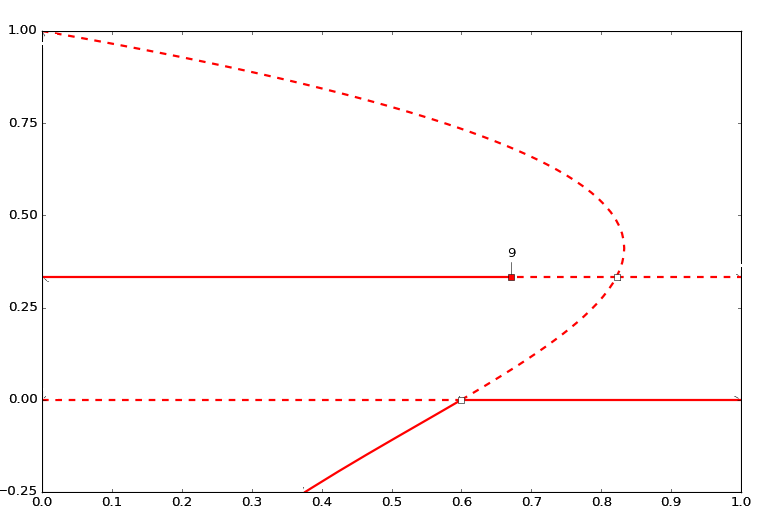
\includegraphics[width=\textwidth]{pp21.png}
  	\caption{Diagrama de bifurcaciones $x-\alpha$ final.}
  \end{figure}
  
\section{Otros diagramas de bifurcaciones}

En este último apartado vamos a representar un par de modelos relacionados con los estudiados en el tema 2.

\subsection{Van der Pol}

En lo que a osciladores se refiere hemos estudiado las cualidades del modelo éstandar. Sin embargo debido a la precisión que requiere el uso de programas como AUTO, vamos a tratar en este apartado una modificación del mismo. Cualitativamente ambos presentan una bifurcación de Hopf con una evolución similar.
Presentamos el modelo:

\begin{equation}
\left \{ \begin{matrix} x'=y-(\frac{1}{3}x^3)-x\\ y'=\epsilon(\alpha-x)\end{matrix}\right . .
\end{equation}  

Como se puede comprobar es una variación del modelo \ref{vanderpol2} en la que optamos por fijar nuestro parámetro en 1 y añadir dos parámetros.El denotado por $\epsilon$ lo fijaremos con antelación y moveremos el parámetro $\alpha$. 

En estos casos, tanto la aplicación de nuestro criterio como la visualización gráfica nos dejan entreveer la aparición de una bifurcación de Hopf.
Por tanto procedemos a escribir el código correspondiente en AUTO y ejecutarlo.

En primer lugar tenemos la salida por pantalla que nos proporciona la verificación de la existencia de una bifurcación de Hopf (mostramos el extracto):

\begin{lstlisting}
BR    PT  TY  LAB    PAR(2)        L2-NORM         
1    16  HB    2   1.00000E+00   1.20185E+00   1.00000E+00  -6.66667E-01
\end{lstlisting}

Y posteriormente, para un análisis completo, podemos usar un visualizador como XPPAUT (código en el apéndice) cuyo núcleo para representar bifurcaciones es AUTO, para visualizar gráficamente los datos: \ref{vandedia}.


 \begin{figure}[h]
 	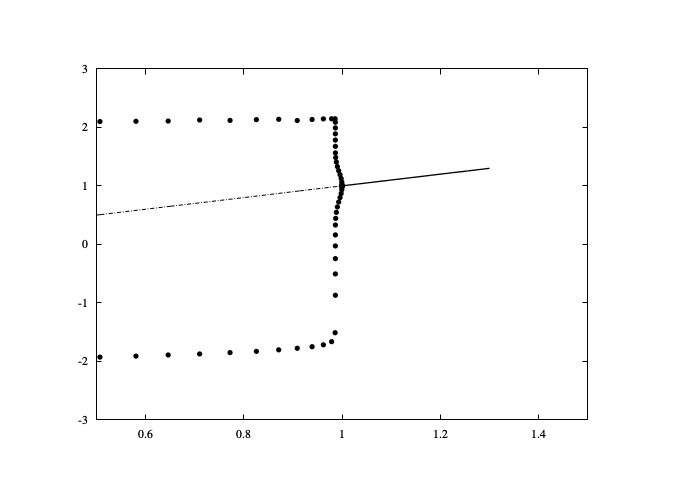
\includegraphics[width=\textwidth]{diagramfinalfinal.png}
 	\caption{Diagrama de bifurcaciones para el modelo \ref{vanderpol}, ejes:  $x-\alpha$ }
 	\label{vandedia}
 \end{figure}

\subsection{Gusanos de las píceas.}

Para completar el trabajo, como el modelo de Sel'kov también experimenta una bifurcación de Hopf, preferimos representar el diagrama de bifurcación fold que experimenta el modelo de ecología \ref{gusaca}.

Este diagrama no es un diagrama \ref{gusacaca}  de bifurcación fold propiamente dicho, pues existen 3 puntos fijos en nuestro sistema. Sin embargo, es apreciable como si nos fijamos en las dos ramas superiores observamos lo que si se corresponde con un diagrama de bifurcación fold. Esto corresponde unívocamente con nuestro problema. 

De nuevo en este caso hemos recurrido a un recurso electrónico para el dibujo, aún así los ficheros con las ecuaciones se adjuntan en el apéndice y pueden ser consultados.

 \begin{figure}[h]
 	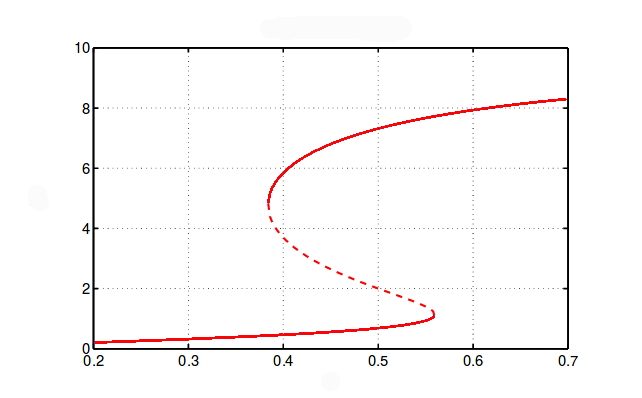
\includegraphics[width=\textwidth]{diagramagusanos.png}
 	\caption{Diagrama de bifurcaciones para el modelo \ref{gusaca}, ejes: $x-r$}
 	\label{gusacaca}
 \end{figure}











\chapter{Conclusiones}

\label{ch:conclusions}

\section{La matemática aplicada}

Las asignaturas que más disfruté en la carrera eran las de matemática aplicada. Y el motivo de ello se puede ver reflejado en este trabajo. 

Estamos ante una rama que une la matemática con nuestra realidad, con aplicaciones de teorías que dan respuestas a preguntas de nuestro alrededor. Pero, lo que es más fascinante, recurre de todas las demás ramas de la matemática, a multitud de herramientas.

Durante este proyecto he trabajado con análisis real, complejo, numérico, geometría, topología, computación...
Y aunque esto haya supuesto una tarea por la que me haya podido sentir sobrepasado en muchos casos, ha sido genial poder ver en armonía y aplicación tantos conceptos.

Además, me gustaría resaltar como sólo he vislumbrado un bosquejo del gran campo de las bifurcaciones, o de la teoría de continuación, o incluso de partes tan particulares como las funciones test. Sin duda uno de las mayores dificultades a las que me enfrenté fue la dificultad de idear un trabajo que sintetizase todo lo que creía conveniente contar, aportando ejemplos reales y algunas demostraciones para mostrar una buena comprensión. 

Al final del mismo, puede que mi enfoque no sea el más correcto, o que existan, según la persona que esté leyendo esto, otras formas de contar y presentar lo expuesto. Aun así, estoy satisfecho con el resultado y con la cantidad de conceptos aprendidos. 



\section{El software matemático}
Una de las primeras conclusiones a destacar es la necesaria renovación del software matemático.
Es habitual que en clase se nos enseñe con programas de código libre, pero esto presenta dos inconvenientes:
Primero, exige estar en constante cambio y evolución. Esto se puede notar en los códigos de este trabajo, alejados del software que nos enseñan, en pos de lenguajes que evolucionan y cada vez tienen más y mejores paquetes. 
Segundo, es habitual que los programas de software libre especializados no contengan tanto soporte y documentación como los privativos.

Lejos de ser una crítica, me parecen puntos a mejorar. AUTO es un lenguaje con una curva de aprendizaje que al principio parece tener pendiente infinita cuya última actualización fue en 2007. Y aún así, la mayoría de aplicaciones son intérpretes del mismo.

Surge como alternativa XPPAUT, y aunque es algo más agradable en cuanto a la creación de código, visualmente deja mucho que desear.


\section{El arte de encontrar parámetros}
Durante este proyecto me he enfrentado a multitud de escollos que he tenido que ir superando, pero, sin ninguna duda, las mayores decepciones han venido de la mano de los parámetros.

Uno puede pensar que la realización de diagramas de bifurcaciones de modelos sencillos no debiera er complicada, pero se equivoca. Es habitual que en la literatura no se trabajen con estos diagramas, ya sea por la dificultad y horas que debemos emplear en ellos o, por supuesto, por claridad, puesto que habitualmente es necesario tener un bagage matemático extenso para que se entienda que estamos representando. 

Nos encontramos entonces ante un camino árduo y muchas veces desechado.

La otra opción podría consistir en consultar papers publicados. Sin embargo, aunque en ellos suelan venir los datos de los parámetros (recalco \emph{los parámetros}, pues para escribir el programa son necesarios muchos más datos como la longitud de paso o las condiciones iniciales), en general los sistemas que hoy en día se tratan poseen varios parámetros y muchas mas ecuaciones.

Este trabajo me ha dado una perspectiva nueva sobre el análisis numérico, mostrándome como la matemática aplicada debe nutrirse de esfuerzo, ensayos, errores y tiempo para que podamos obtener resultados. También ha supuesto un refrescante contacto con la vida real, en la que a menudo no se buscan soluciones exactas (porque no suelen encontrarse) y en la que las respuestas (que ya no son blanco o negro) deben estar sometidas a constante revisión.





\appendix
\chapter{Códigos AUTO}\label{aped.A}
\section{Código del modelo predador presa.}
Versión modificada original en \cite{auto}. 
Comandos:
\begin{lstlisting}
#Archivo.auto
pp2 = run('pp2')
save('pp2')
clean()
\end{lstlisting}
Archivo de ecuaciones:
\begin{lstlisting}
SUBROUTINE FUNC(NDIM,U,ICP,PAR,IJAC,F,DFDU,DFDP) 
!--------- ---- 

IMPLICIT NONE
INTEGER, INTENT(IN) :: NDIM, IJAC, ICP(*)
DOUBLE PRECISION, INTENT(IN) :: U(NDIM), PAR(*)
DOUBLE PRECISION, INTENT(OUT) :: F(NDIM)
DOUBLE PRECISION, INTENT(INOUT) :: DFDU(NDIM,*), DFDP(NDIM,*)

DOUBLE PRECISION e

e=EXP(-PAR(3)*U(1)) 

F(1) = U(2)
F(2) = PAR(1)*U(1)*U(1)*U(2)-PAR(1)*U(2)-U(1)

END SUBROUTINE FUNC
!-------------------------------------------------------

SUBROUTINE STPNT(NDIM,U,PAR,T) 
!--------- ----- 

IMPLICIT NONE
INTEGER, INTENT(IN) :: NDIM
DOUBLE PRECISION, INTENT(INOUT) :: U(NDIM), PAR(*)
DOUBLE PRECISION, INTENT(IN) :: T

PAR(:4) = (/ 0.0, 3.0, 5.0, 3.0 /)
U = 0.0

END SUBROUTINE STPNT
!-------------------------------------------------------

SUBROUTINE PVLS(NDIM,U,PAR)
END SUBROUTINE PVLS

SUBROUTINE BCND 
END SUBROUTINE BCND

SUBROUTINE ICND 
END SUBROUTINE ICND

SUBROUTINE FOPT 
END SUBROUTINE FOPT
\end{lstlisting}
Archivo de constantes (proporcionado en \cite{auto})

\begin{lstlisting}
NDIM=2
unames={1: 'presa', 2: 'predador'}
parnames={1: 'alpha', 9: 'presa'}
NPR=100
ICP=['alpha']
UZSTOP={'alpha': [0.0, 30.0], 'presa': -0.25}, NMX=100
IPS=1, IRS=0
DS=0.02, DSMIN=0.01, DSMAX=0.06
NTST=90
\end{lstlisting}
\section{Código Van der Pol modificado}
Archivo auto generado por VFGEN. Archivo original y constantes en

 \hyperlink{VFGEN}{http://www.warrenweckesser.net/vfgen/}
\begin{lstlisting}
<?xml version="1.0" ?>
<VectorField
Name="oscilador" >
<Parameter
Name="epsilon"
DefaultValue="0.2" />
<StateVariable
Name="x"
Formula="(y+x-x^3/3.0)/epsilon"
DefaultInitialCondition="0.01" />
<StateVariable
Name="y"
Formula="-x"
DefaultInitialCondition="0" />
</VectorField>
\end{lstlisting}
Versión en XPPAUT,versión de Anna M. Barry en ResearchGate.
\begin{lstlisting}
init x=2 y=4
par eps=0.1 a=1.3
x_0 = y - (1/3 * x 3 - x)
y_0 = eps * (a - x)
@ dt=.025, total=100, xplot=x,yplot=y, axes=2d
@ xlo=-3, xhi=3, ylo=-3, yhi=3
@ maxstor=20000
done
\end{lstlisting}

\section{Código Van der Pol éstandar }
Código de XPPAUT para ejecutar en AUTO. No he hallado el archivo de datos original para completar el diagrama completo.
\begin{lstlisting}
x' = y
y' = -beta*(x^2-1)*y - x
par beta=1.0
init x=1.0  y=0.0 
@ xplot=x, yplot=y
@ total=10,dt=.01,xlo=-3.0,xhi=3.0,ylo=-3.0,yhi=3.0
done
\end{lstlisting}
\chapter{Códigos Python}\label{aped.B}
\section{Dibujar órbitas}
Basado en \hyperlink{DropBearCode}{http://dropbearcode.blogspot.com}
\begin{lstlisting}
#Librerias
import numpy as np
import matplotlib.pyplot as plt
from scipy.integrate import odeint

#Condiguracion de imagen
fig = plt.figure(figsize=(8,8))
ax=fig.add_subplot(111)

#Sistema
def ecuacion(x, t):
nx0 = primera_componente
nx1 = segunda_componente
res = np.array([nx0, nx1])
return res

#mallado
ts = np.linspace(0.0, 50.0, 500)

#Rama
xs = odeint(ecuacion, [parametro_superior, parametro_inferior], ts)

#Representacion
plt.plot(xs[:,0], xs[:,1])
plt.gca().set_aspect('equal')
plt.show()
\end{lstlisting}
\section{Nulclinas y diagrama de fases}
\begin{lstlisting}

#Librerias
import matplotlib.pyplot as plt
import matplotlib.patches as mpatches
from scipy import *
from scipy import integrate
from scipy.integrate import ode
import numpy as np
import math

#configuracion de imagen
fig = plt.figure(figsize=(8,8))
ax=fig.add_subplot(111)

#Marcas para la leyenda
red_patch = mpatches.Patch(color='red',label='Nuclina de $y$')
blue_patch = mpatches.Patch(color='blue',label='Nuclina de $x$')
black_patch = mpatches.Patch(color='black',label='Diagrama de fases')


#Soluciones
h = linspace(-2,3,400)
a=0*h
b=-h**3/3+h

#campo de vectores
X,Y = np.meshgrid( np.linspace(-2,5,30),np.linspace(-2,5,30) )
U = -Y-X*X*X/3+X
V = X

#script para normalizar vectores
N = np.sqrt(U**2+V**2)  
U2, V2 = U/N, V/N
ax.quiver( X,Y,U2, V2,cmap=plt.cm.jet)

##diagrama 
plt.plot()
plt.plot(h,a,'r')
plt.plot(h,b,'b')
plt.xlim([-2,3])
plt.ylim([-1,1.5])
plt.xlabel(r"$x$")
plt.ylabel(r"$y$")
plt.legend(handles=[red_patch,blue_patch,black_patch])
\end{lstlisting}
Modifíquese si sólo se quiere obtener una de las dos cosas. Todos los diagramas de fases están realizados con ese script.

\chapter{Códigos Geogebra}\label{aped.C}
\section{Archivo de visualización dinámica}
\begin{lstlisting}
Declaracion de funciones

f=Funcion[ <Funcion>, <Valor de x Inicial>, <Valor de x Final> ]
g=Funcion[ <Funcion>, <Valor de x Inicial>, <Valor de x Final> ]

Diagrama de fases (vectores normalizados)

Secuencia[Secuencia[Vector[(i, j), (i, j) + 0.15(f(i, j), g(i, j)) / sqrt(f(i, j)^2 + g(i, j)^2)], i, ext_inic, ext_fin, tam_paso], j, ext_inic, ext_fin, tam_paso]

Resolucion para orbitas:
ResuelveEDO[g, f, punto_inic, punto_fin, tiempo final, tam. de paso]


\end{lstlisting}

\addcontentsline{toc}{chapter}{Bibliografía}
\bibliographystyle{alpha}
\bibliography{bibliography/bibliografia}

\end{document}
